%% --------------------------------------------------------------------
%% Template UTEC Tesis
%% --------------------------------------------------------------------
% Este es el archivo que se debe compilar.
% 
% Este template ha sido modificado y actualizado por Eduardo Castro y Roosevelt Ubaldo en base a lo trabajado por Víctor Murray, Oscar Ramos y Juan Carlos Barbaran.
%
% Última actualización: Mayo, 2022

\documentclass[a4paper,12pt,oneside]{tesisutec}

\selectlanguage{spanish}
\usepackage{pgfgantt}
\usetikzlibrary{positioning, arrows.meta, shapes.geometric}
\usepackage{pdflscape}

%%añadidos por mi
\usepackage{placeins}
\usepackage{enumitem}
\usepackage{multirow}
\usepackage[table]{xcolor}



%% Paquetes
\usepackage[T1]{fontenc}
\usepackage[utf8]{inputenc}
\usepackage[square, numbers, comma, sort&compress]{natbib}
%Libreria para codigo
\usepackage{listings}
% Ajustar los parámetros de lstlisting
\lstset{
    basicstyle=\ttfamily\small,
    breaklines=true,
    frame=single,
    xleftmargin=2em,  % margen izquierdo
    xrightmargin=2em,  % margen derecho
    language=Python,
    captionpos=b,
    tabsize=3,
    frame=lines,
    numbers=left,
    numberstyle=\tiny,
    numbersep=5pt,
    breaklines=true,
    showstringspaces=false,
    basicstyle=\footnotesize,
    %identifierstyle=\color[rgb]{0.3,0.133,0.133},
    %keywordstyle=\color[rgb]{0.133,0.133,0.6},
    %stringstyle=\color[rgb]{0.133,0.533,0.133},
    %commentstyle=\color[rgb]{0.133,0.133,0.133},
}
% Libreria de idioma
\usepackage[spanish]{babel}
% Libreria para posicionamiento
\usepackage{float}
% Librerias para insertar codigos
\usepackage[spanish,onelanguage,ruled,vlined]{algorithm2e}
\usepackage{verbatim} 
% Librería para hipervínculos
\usepackage{hyperref}
 % Librería necesaria para arreglar el orden de referencias en overleaf.com
\usepackage{notoccite}

% Incluir acá los paquetes adicionales que deseas. 
% Ubicación de los imágenes.
\graphicspath{images/}

\makeatletter
% Reinsert missing \algbackskip
\def\algbackskip{\hskip-\ALG@thistlm}
\makeatother

\hypersetup{urlcolor=blue, colorlinks=true}

\begin{document}

\department{INGENIERÍA MECATRÓNICA}
\degree{Bachiller }
\major{Ingeniería Mecatrónica}

\title{Diseño e implementación de un sistema IoT multivariable de monitoreo, alerta y control comparativo (CO\(_2\), material particulado, temperatura y humedad) para espacios universitarios, basado en comunicación LoRa mediante un gateway personalizado}


\author{
    Sebastián André Peralta Ibañez (ORCID: 0009-0002-0417-8626)\\
    Gianni Francesco Vaccaro Ortiz (ORCID: 0009-0002-0417-8622)
}% Es obligatorio agregar ORCID del alumno


\supervisor{Milenka Karolyn Gamero Tornero} % Es obligatorio agregar ORCID del asesor

\date{2026}

\maketitle

\frontmatter

\setstretch{1.5}


%% ============================================================================
%  Dedicatoria
%% ============================================================================

\dedicatory{
Dedicamos este trabajo a nuestros padres, por su apoyo incondicional, esfuerzo y confianza durante todo nuestro proceso de formación académica. Su acompañamiento ha sido fundamental para alcanzar esta etapa y culminar el presente proyecto de tesis.
}

%% ============================================================================
%  Pagina de Agradecimientos
%% ============================================================================

\acknowledgements{

Agradecemos, en primer lugar, a nuestros padres, por su constante apoyo, comprensión y motivación a lo largo de nuestra formación universitaria. Su respaldo fue fundamental para el desarrollo y culminación de este trabajo de tesis.

Asimismo, expresamos nuestro sincero agradecimiento a nuestra asesora, Milenka Karolyn Gamero Tornero, por su orientación, paciencia y acompañamiento durante el desarrollo del proyecto. Sus recomendaciones y observaciones contribuyeron significativamente a mejorar la calidad técnica y académica de la investigación.

Finalmente, agradecemos a la Universidad de Ingeniería y Tecnología -- UTEC por brindarnos las facilidades necesarias para la ejecución del proyecto, incluyendo el acceso a aulas, espacios de prueba e instrumentos requeridos para la implementación y validación del sistema propuesto.

}



\tableofcontents

\newpage

\listoftables

\newpage

\listoffigures

\addtocontents{toc}{\vspace{1.5em}}

%% ============================================================================
\mainmatter
\pagestyle{fancy}

\customchapter{RESUMEN}

La calidad del aire en espacios cerrados, especialmente en aulas universitarias, es crucial para el bienestar y el rendimiento de los estudiantes. Altos niveles de dióxido de carbono (CO\(_2\)) y material particulado (polvo), sumados a variaciones de temperatura y humedad, pueden afectar negativamente la salud y el desempeño cognitivo de los ocupantes. En este contexto, este trabajo presenta el diseño e implementación de un sistema de monitoreo ambiental multivariable y alerta en tiempo real basado en una arquitectura de red de Internet de las Cosas (IoT). El sistema está compuesto por nodos sensores que recopilan mediciones de CO\(_2\), polvo, temperatura y humedad, transmitiéndolas vía comunicación inalámbrica LoRa hacia un gateway personalizado basado en ESP32. Este gateway actúa como puente para enviar los datos hacia una infraestructura en la nube, desplegada en Microsoft Azure mediante Infraestructura como Código (IaC). La plataforma web para la visualización ha sido desarrollada utilizando React, acoplada a una API alojada en Azure Container Apps, y los datos se almacenan en Azure Cosmos DB. El sistema incluye la generación de alertas automatizadas y un subsistema de mitigación activa que compara el rendimiento de diversas estrategias de control de ventilación (tales como PID, entre otras) cuando se exceden los umbrales permisibles, contribuyendo a la creación de ambientes educativos más seguros. Las pruebas de integración validaron el flujo de datos completo y su capacidad para monitorear y accionar medidas de mitigación en tiempo real.

\noindent \textbf{Palabras clave:}\\
\noindent Calidad del aire; CO\(_2\); material particulado; temperatura; humedad; IoT; LoRa; Azure; control comparativo; ventilación automatizada.
\customchapter{ABSTRACT}

The air quality in enclosed spaces, especially classrooms, is crucial for the well-being and performance of individuals. High levels of carbon dioxide (CO\(_2\)) can affect the health and cognitive performance of occupants. In this context, this work presents the design and implementation of a real-time monitoring and alert system for CO\(_2\) levels in classrooms using LoRa wireless communication in an Internet of Things (IoT) network. The system is composed of sensor nodes that collect and send data to a central server, where they are stored and processed in the cloud using Amazon Web Services (AWS). The web platform for data visualization and monitoring was developed using .NET, and the collected information is stored in a database managed with SQL Server. The system includes the generation of alerts when CO\(_2\) levels exceed permissible limits, contributing to the creation of safer and healthier educational environments. Tests of the system in selected classrooms validated its ability to monitor and alert in real time.

\noindent \textbf{Keywords:}\\
\noindent CO\(_2\); IoT; LoRa; .NET; AWS; SQL Server; real-time monitoring; air quality; classrooms.

\customchapter{INTRODUCCIÓN} 

\section{Presentación del tema de investigación}

La calidad del entorno en espacios interiores, conocida como Calidad Ambiental Interior (IEQ, por sus siglas en inglés), abarca una diversidad de elementos que influyen en el ambiente, incluyendo el confort térmico, la calidad del aire, las condiciones acústicas y el confort visual, entre otros aspectos como el diseño interior o la ubicación del edificio \cite{source1}. De estos componentes, el confort térmico, la calidad del aire interior (CAI), la acústica y el confort visual son los que se pueden monitorear físicamente y se consideran particularmente relevantes para la salud y productividad de las personas \cite{source1}.

La relevancia de mantener una adecuada calidad del aire interior se justifica dado que la mayoría de las personas pasan alrededor del 90\% de su tiempo en estos ambientes \cite{its_about_time_a_comparison_of_canadian_and_american_time_activity_patterns}. En este contexto, entre los principales enfoques de los sistemas de monitoreo de la calidad de aire en espacios cerrados desde el año 2015 está la medición y seguimiento de los niveles de dióxido de carbono (CO\(_2\)), los cuales se realizan en un 65\% de ellos \cite{IAQ_monitoring_systems_based_on_internet_of_things_a_systematic_review}. El interés por este parámetro se debe a la relación que existe entre los altos niveles de CO\(_2\) y distintos efectos perjudiciales a nivel fisiológico y psicomotor \cite{effects_of_low_level_inhalation_exposure_to_carbon_dioxide_in_indoor_environments_a_short_review_on_human_health_and_psychomotor_performance}.

Debido a esta importancia, tanto organizaciones internacionales como nacionales han emitido regulaciones sobre los niveles de CO\(_2\) en espacios cerrados. La base de datos de la Sociedad Internacional de la Calidad del Aire Interior y Clima (ISIAQ) indica que la moda del valor máximo permitido de CO\(_2\) en interiores es de 1000 ppm, con rangos que varían entre 700 ppm y 1500 ppm \cite{indoor_air_quality_guidelines_from_across_the_world_an_appraisal_considering_energy_saving_health_productivity_and_comfort, ISIAQ_database}. En el ámbito nacional peruano, la directiva administrativa N°349-MINSA/DGIESP-2024 señala que un umbral adecuado de concentración de CO\(_2\) es 400 ppm sobre el nivel de base (ambiente sin personas), y es deseable que no se sobrepasen las 1000 ppm \cite{directiva_minsa}.

Tradicionalmente, la evaluación de la IEQ ha sido una tarea compleja que requería equipos especializados de grado científico y procedimientos de medición detallados \cite{source1}. Sin embargo, la reciente aparición en el mercado de monitores ambientales de bajo costo basados en el Internet de las Cosas (IoT) ha generado un creciente interés en la comunidad científica para evaluar su potencial \cite{source1}. Estos dispositivos, a menudo en un rango de precio de hasta 500 EUR, con la mayoría situándose entre 200 y 350 EUR, prometen una mayor accesibilidad \cite{source1}.

Si bien gran parte de la investigación con estos dispositivos económicos se ha centrado en la calidad del aire interior, especialmente en la detección de partículas, algunos estudios han ampliado el alcance para incluir otros parámetros como el CO\(_2\), compuestos orgánicos volátiles totales (VOCs), temperatura y humedad relativa \cite{source1}. El tema es de particular relevancia en ingeniería debido a la creciente adopción de tecnologías IoT en sectores como el cuidado de la salud y la educación. El IoT constituye soluciones tecnológicas mediante la integración de sensores y otros componentes de hardware en un ecosistema que les permite interactuar para gestionar datos y acciones \cite{the_application_of_internet_of_things_in_healthcare_a_systematic_literature_review_and_classification}. Proyectos que exploran el uso de tecnología IoT para el monitoreo ambiental tanto en interiores como exteriores, utilizando plataformas como Arduino, Raspberry Pi y tecnologías de comunicación como LoRaWAN, han sido desarrollados \cite{source3, source5, source6, source8}, con visualización de datos a través de plataformas IoT especializadas \cite{source3, source5, source8, source12}.

No obstante, el consumo energético es una preocupación principal en aplicaciones de monitoreo en tiempo real, determinado predominantemente por el protocolo de comunicación \cite{IAQ_monitoring_systems_based_on_internet_of_things_a_systematic_review}. Alternativas de bajo consumo como Bluetooth o ZigBee son utilizadas para áreas reducidas debido a limitaciones de alcance. Tecnologías de largo alcance como Wi-Fi pueden no ser deseables para implementaciones como un campus inteligente debido a su alto consumo energético. Para tales aplicaciones, se requiere un protocolo adecuado en términos de consumo y alcance, como LoRa, que cumple estos requerimientos para distancias de pocos kilómetros \cite{source3, source5, source9, source10}.

Un enfoque holístico para la evaluación de la IEQ es fundamental para entender la interacción entre sus diversos componentes y para desarrollar un índice unificado de IEQ, que incluya coeficientes de ponderación que reflejen la importancia mutua de estos factores \cite{source1}. Este proyecto de investigación se enmarca en este contexto, buscando desarrollar un índice de IEQ y un prototipo de sistema de monitoreo IoT accesible y funcional, utilizando tecnología LoRa, para evaluar la calidad ambiental en espacios cerrados dentro de un campus universitario.























\section{Descripción de la situación problemática}

A pesar del reconocimiento de la importancia de la Calidad Ambiental Interior (IEQ) para la salud y la productividad \cite{source1}, su monitoreo tradicional ha sido costoso y poco accesible para el usuario común debido al uso de equipos especializados y procedimientos complejos \cite{source1}. La aparición de monitores IoT de bajo costo ha comenzado a cambiar este panorama, democratizando la posibilidad de medir parámetros ambientales \cite{source1}. Tras la pandemia de SARS-CoV-2, que reveló vulnerabilidades y la falta de controles adecuados, el monitoreo de los niveles de CO\(_2\) ha adquirido una relevancia aún mayor, no solo por sus efectos adversos, sino también porque es un indicador clave del riesgo de contagio en ambientes cerrados.

Sin embargo, la mayoría de las evaluaciones y el desarrollo de estos dispositivos económicos se han centrado principalmente en componentes individuales de la IEQ, como la calidad del aire interior, a menudo limitándose al monitoreo de partículas o dióxido de carbono \cite{source1}. Actualmente, no existe en el mercado un monitor de grado de consumo que ofrezca una evaluación holística de la IEQ, integrando mediciones de diversos parámetros ambientales de manera comprensiva \cite{source1}.

Muchos de los proyectos de monitoreo de IEQ con dispositivos de bajo costo, como los basados en Arduino, se encuentran en etapas de prueba de concepto, y su rendimiento y fiabilidad en despliegues reales a gran escala aún no están completamente documentados o garantizados \cite{source1}. La necesidad de medir la IEQ de manera integral es crucial para poder caracterizar la importancia de sus componentes e integrar esta información en un índice unificado que sea fácil de interpretar \cite{source1}.

Específicamente en entornos educativos como las universidades, mantener una buena calidad ambiental interior es un desafío relevante. Estudios sobre la calidad del aire en salones universitarios han identificado espacios con concentraciones de CO\(_2\) que superan los límites admisibles, lo que puede generar malestar físico en los estudiantes y aumentar el riesgo de transmisión de virus \cite{source23}. Aunque se han implementado sistemas de monitoreo, la cobertura total de los espacios, la integración de diversas variables ambientales más allá del CO\(_2\), y el uso de equipos con alta precisión o capacidades avanzadas de análisis pueden requerir una inversión significativa \cite{source23, source24}. La facilidad de uso y la accesibilidad de la información para los ocupantes finales también son aspectos a mejorar en los sistemas existentes \cite{source1}.

En este contexto, la situación problemática se centra en la brecha existente entre la necesidad de un monitoreo integral y accesible de la IEQ en espacios universitarios y la disponibilidad actual de soluciones tecnológicas que sean a la vez de bajo costo, holísticas, fáciles de usar e implementar.








\introsection{Formulación del problema}

%El presente proyecto se centra en el diseño e implementación de una alternativa de robot de vigilancia y patrullaje capaz de identificar intrusos mediante procesamiento de imágenes. Para ello se escogió un robot de dos ruedas de tipo péndulo invertido, pues permite operar con mayor facilidad en espacios estrechos, y hacerlo con mayor rapidez que un robot de cuatro ruedas, lo que le permite adaptarse mejor a la estructura de las instalaciones en las que será usado \cite{TWR_advantages}. Para controlar el robot, se seleccionó el controlador adaptativo por modelo de referencia directo (MRAC directo) debido a que es un algoritmo de control robusto que permite controlar el robot sobre distintas superficies. Con respecto a los algoritmos de procesamiento de imágenes para patrullaje y detección de intrusos se seleccionó el clasificador Haar Cascade para detección de personas y el algoritmo de localización y el algoritmo de localización y mapeo simultáneos (SLAM) para ubicar el lugar las detecciones en el mapa de las instalaciones. Para incrementar la tasa de cuadros por segundo procesados, se implementó parte de los algoritmos de procesamiento de imágenes en lógica programable, es decir, circuitos lógicos secuenciales reconfigurables, como los FPGA (Field-Programmable Gate Arrays).

Dado el impacto de los altos niveles de CO\(_2\) en la salud y el rendimiento académico, especialmente en entornos cerrados como aulas, surge la pregunta: ¿Cómo podemos diseñar e implementar un sistema de monitoreo basado en IoT que mida, registre y alerte sobre los niveles de CO\(_2\) en tiempo real, asegurando que los ambientes educativos se mantengan dentro de los límites saludables establecidos?


\introsection{Objetivos de investigación}
En esta sección se presentan los objetivos de este Trabajo Final de Ingeniería Mecatrónica. Sobre ellos se estructuró la investigación y los resultados presentados.

\subsubsection*{Objetivo general}
Desarrollar un Índice de Calidad Ambiental Interior (IEQ) e implementar un prototipo funcional de sistema de monitoreo IoT basado en LoRa, compuesto por tres nodos sensores, para la evaluación y visualización de la calidad ambiental en espacios cerrados dentro de un campus universitario.

\subsection*{Objetivos Específicos}

\begin{itemize}
    \item Analizar la literatura científica y normativa referente a los parámetros clave de la calidad ambiental interior (CO\(_2\), material particulado PM\textsubscript{2.5}, temperatura y humedad), incluyendo sus umbrales de referencia y las metodologías existentes para la formulación de índices de calidad ambiental.
    \item Establecer sub-índices para los parámetros ambientales seleccionados (CO\(_2\), PM\textsubscript{2.5}, temperatura y humedad), determinando rangos y sistemas de puntuación fundamentados en la literatura científica para categorizar los niveles de calidad o confort.
    \item Desarrollar una metodología de ponderación y agregación, claramente justificada, para los sub-índices definidos, orientada a la obtención de un Índice de Calidad Ambiental Interior (IEQ) unificado, simplificado y de fácil interpretación.
    \item Diseñar la arquitectura e implementar un prototipo funcional de un sistema de monitoreo ambiental IoT, empleando tecnología LoRa para la comunicación inalámbrica de datos desde tres nodos sensores (para la medición de CO\(_2\), PM\textsubscript{2.5}, temperatura y humedad) hacia un dispositivo gateway.
    \item Configurar la transmisión de datos desde los nodos sensores hacia el gateway y, subsecuentemente, a una plataforma en la nube para su almacenamiento básico y visualización.
    \item Incorporar el IEQ formulado en la plataforma de visualización del prototipo, habilitando la observación en tiempo real del índice calculado a partir de los datos adquiridos por los sensores.
    \item Ejecutar pruebas funcionales del prototipo implementado para validar la correcta recolección, transmisión, almacenamiento y visualización de datos, así como el cálculo del IEQ, en espacios seleccionados del campus universitario.
    \item Elaborar la documentación técnica detallada del diseño del IEQ, su fundamentación teórica, la arquitectura e implementación del prototipo del sistema de monitoreo IoT-LoRa (incluyendo nodos y gateway), los resultados de las pruebas funcionales, y las consideraciones para su aplicabilidad y potencial escalabilidad en un entorno universitario.
\end{itemize}


\introsection{Justificación}

%Desarrollar este proyecto permite contar con una alternativa de robot de patrullaje y vigilancia capaz de ejecutar el algoritmo de detección de intrusos en el mismo robot a una mayor tasa de cuadros por segundo gracias a la aceleración por hardware. Esta alternativa resulta particularmente útil para casos en los que el territorio extenso, no se cuenta con una red WI-FI local a la cual conectarse para hacer el procesamiento de imágenes en una computadora física y no es viable instalar un router portátil en el robot debido a que no hay cobertura de servicios de internet, como en zonas rurales, o no se desea enviar los datos a la nube para su procesamiento.

La calidad del aire en espacios cerrados ha adquirido gran importancia en los últimos años debido a los riesgos que altos niveles de CO\(_2\) representan para la salud humana y la productividad. Estudios recientes han demostrado que concentraciones elevadas de CO\(_2\) en interiores no solo afectan el rendimiento cognitivo y físico, sino que también son un indicador clave del riesgo de contagio y proliferación de microorganismos, un aspecto que ha cobrado relevancia tras la pandemia de SARS-CoV-2.

En el ámbito educativo, donde estudiantes y docentes pasan la mayor parte del tiempo en salones de clase, es esencial garantizar una adecuada calidad del aire. Sin embargo, muchos centros educativos no cuentan con sistemas de monitoreo que permitan medir en tiempo real los niveles de CO\(_2\), lo que puede derivar en ambientes no saludables que impactan negativamente tanto en el bienestar como en el rendimiento académico.

A pesar de los avances en tecnología IoT, la implementación de redes de monitoreo eficientes sigue siendo un reto. Este proyecto se enfoca en diseñar e implementar una red IoT de nodos sensores para medir los niveles de CO\(_2\) en aulas, recopilando esta información en una base de datos en la nube. El objetivo es poder alertar de manera oportuna cuando se sobrepasen los límites de CO\(_2\) permitidos, asegurando que el ambiente sea siempre apto para las personas, y así contribuir a la creación de entornos educativos más seguros y saludables, en línea con las regulaciones nacionales e internacionales vigentes sobre calidad del aire en interiores.


\subsection*{Alcances y Limitaciones}

El alcance del proyecto comprende el diseño teórico del Índice de Calidad Ambiental Interior (IEQ) y la implementación de un prototipo funcional del sistema de monitoreo IoT-LoRa. Se definirán los parámetros del IEQ (CO\(_2\), PM\textsubscript{2.5}, temperatura y humedad), sus rangos y la metodología de cálculo basada en la revisión de literatura científica y estándares existentes. Asimismo, se implementará un prototipo con tres nodos sensores que medirán los parámetros definidos, utilizando tecnología LoRa para la comunicación inalámbrica con un gateway, y se configurará la transmisión de datos desde los nodos al gateway y de este a una plataforma en la nube para su almacenamiento básico y visualización, donde se mostrará el IEQ calculado. Las pruebas funcionales del prototipo se realizarán en un número limitado de espacios cerrados dentro del campus universitario para demostrar su operatividad. Es importante destacar que no se contempla la construcción de carcasas o gabinetes protectores para los nodos sensores ni para el gateway del prototipo, y la validación del IEQ se basará en su fundamentación teórica y en la coherencia de los resultados del prototipo durante las pruebas funcionales, sin incluir estudios de percepción de confort con ocupantes.

Las limitaciones del proyecto incluyen principalmente el factor tiempo, ya que el desarrollo está restringido a un periodo de 7 semanas, lo que condiciona la profundidad de la experimentación, el número de nodos a implementar y la exhaustividad de las pruebas. Adicionalmente, un presupuesto limitado restringe la cantidad y tipo de sensores, fijando el número de nodos sensores en tres para este prototipo, así como la sofisticación de los componentes del gateway y la plataforma de visualización. La implementación física se materializará en un prototipo funcional básico, sin contemplar un despliegue a gran escala ni una optimización para producción masiva; la robustez del hardware estará, por tanto, sujeta a los componentes de bajo costo disponibles y no se diseñarán ni construirán carcasas o gabinetes protectores, lo que podría limitar su durabilidad y protección a largo plazo. En cuanto a la validación del Índice IEQ, esta se limitará a los datos recolectados por el prototipo durante las pruebas funcionales, sin realizar estudios comparativos con equipos de referencia de alta precisión ni encuestas detalladas de percepción de confort a los ocupantes. La definición de umbrales y, especialmente, las ponderaciones para los parámetros del IEQ dependerán de la información disponible y consensuada en la literatura científica. Finalmente, las pruebas funcionales del prototipo se realizarán en un número limitado de espacios dentro del campus universitario, por lo que los resultados podrían no ser generalizables a todos los tipos de recintos sin adaptaciones, y no se realizarán estudios exhaustivos de cobertura de la señal LoRa en todo el campus ni análisis detallados de interferencias.

d

\introsection{Organización del trabajo de investigación}
El plan de trabajo de esta investigación se muestra en la tabla \ref{tab: gantt}.

\begin{table}[H]
\centering
    \caption{\centering Diagrama de Gantt del proyecto.}
    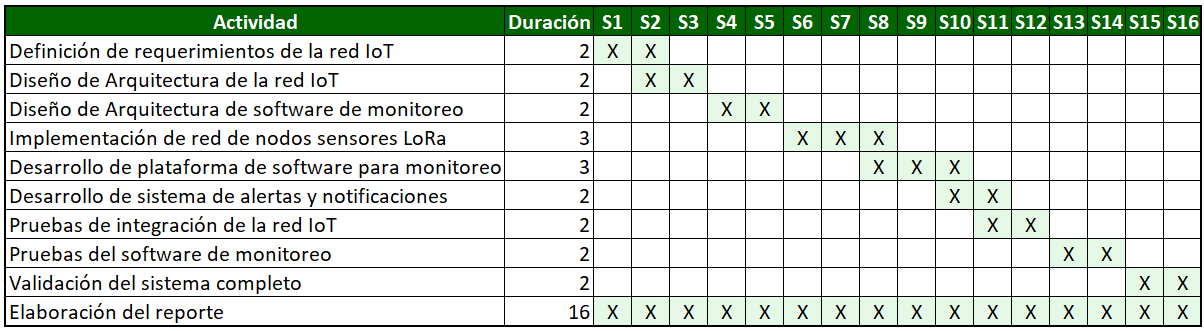
\includegraphics[width=1\linewidth]{images/Introduccion/Gantt.png}
\label{tab: gantt}
\end{table}

Este trabajo de investigación está organizado de la siguiente forma. El Capítulo I, la revisión de la literatura, presenta sistemas de medición y monitoreo de CO\(_2\) en espacios cerrados en proyectos de investigación como estado del arte e investigaciones relacionadas a herramientas de monitoreo manuales de CO\(_2\) u otros sistemas de medición de gases en espacios cerrados como trabajos previos. En el capítulo II, el marco teórico, se presenta tanto la arquitectura de la red IoT que contiene los nodos sensores, así como la arquitectura de software que se utilizará para el programa de monitoreo. En el Capítulo III, el marco metodológico, se presenta la implementación de red de nodos sensores LoRa, el desarrollo de la plataforma de software de monitoreo y el sistema de alertas y notificaciones. En el Capítulo IV, de resultados, se presentan las pruebas de integración de la red IoT, las pruebas del software de monitoreo y el sistema de alertas, y la validación del sistema completo. Por último, se abordan las conclusiones en relación con los objetivos planteados y se hacen recomendaciones para trabajos futuros.

\chapter{REVISIÓN DE LA LITERATURA}

La calidad de los ambientes interiores (IEQ, por sus siglas en inglés), particularmente en entornos educativos, es un factor crítico que afecta directamente el bienestar, la salud, la seguridad y la comodidad de sus ocupantes \cite{lopez_carreno_2025, teba_2021}. Este capítulo presenta una revisión de la literatura científica y técnica relacionada con la evaluación de la calidad ambiental interior, con un enfoque específico en los sistemas de monitoreo de niveles de CO\(_2\) y otros parámetros relevantes en espacios universitarios, así como la integración de tecnologías emergentes como el Internet de las Cosas (IoT) y LoRaWAN. Se exploran los antecedentes en la medición de la calidad del aire, las normativas nacionales e internacionales, los índices de calidad ambiental, y se examinan soluciones recientes de monitoreo basadas en IoT, con énfasis en el uso de tecnologías de comunicación inalámbrica como LoRa y las plataformas de software para la recolección, visualización y análisis de datos. Este análisis permitirá identificar las brechas existentes y fundamentar el diseño propuesto en esta tesis.

\section{Antecedentes de la Calidad Ambiental Interior y su Monitoreo}

\subsection{Definición e Importancia de la Calidad Ambiental Interior}
La calidad del aire de interiores (CAI), un componente crucial de la IEQ, es determinante para la salud respiratoria y el confort de las personas \cite{sandoval_etal_2020}. Más allá de los agentes patógenos, existen otros factores que impactan el bienestar y que pueden ser medidos y controlados \cite{teba_2021}. La norma UNE 171330:2008 define la Calidad Ambiental en Interiores (CAI) como las condiciones ambientales de los espacios interiores adecuadas para el usuario y la actividad, determinadas por los niveles de contaminación química, microbiológica y los valores de los factores físicos, excluyendo recintos de uso industrial o agrícola \cite{teba_2021}.

Altas concentraciones de contaminantes como el dióxido de carbono (CO\(_2\)) en espacios cerrados pueden generar impactos negativos en la salud y aumentar el riesgo de transmisión de enfermedades respiratorias \cite{contreras_perez_2020, effects_of_low_level_inhalation_exposure_to_carbon_dioxide_in_indoor_environments_a_short_review_on_human_health_and_psychomotor_performance}. El CO\(_2\), proveniente principalmente de la respiración humana en espacios no industriales, es un indicador clave de la ventilación \cite{contreras_perez_2020}. Niveles bajos de humedad también pueden favorecer la transmisión de virus, mientras que la temperatura es crucial para el confort y la salud en espacios concurridos \cite{contreras_perez_2020}. La pandemia de COVID-19 resaltó la importancia de la ventilación adecuada, siendo la circulación de aire exterior el mecanismo más efectivo para reducir la concentración de aerosoles potencialmente infecciosos en espacios como aulas \cite{contreras_perez_2020}. La evaluación de la CAI es, por tanto, fundamental para gestionar riesgos y mejorar la experiencia y salud de los ocupantes \cite{contreras_perez_2020, envira_nodate, higiene_ambiental_nodate}.

\subsection{Evolución Histórica del Monitoreo de la Calidad del Aire}
El monitoreo de la calidad del aire ha progresado significativamente desde mediados del siglo XX. En los años 1940, los primeros dispositivos eran rudimentarios, como tiras de caucho que medían ozono por su agrietamiento, pero requerían mantenimiento constante y tenían precisión limitada \cite{The_Evolution_of_Air_Quality_Monitoring}. Posteriormente, se usaron medidores de CO\(_2\) basados en soluciones químicas, aunque con problemas de fugas y calibración \cite{The_Evolution_of_Air_Quality_Monitoring}. La implementación de redes de estaciones de monitoreo continuo, como la de Los Ángeles en los años 50, permitió la recolección continua de datos y la emisión de alertas, sentando las bases para los sistemas modernos \cite{The_Evolution_of_Air_Quality_Monitoring, indoor_air_quality_guidelines_from_across_the_world_an_appraisal_considering_energy_saving_health_productivity_and_comfort}.

En décadas recientes, la tecnología ha permitido sistemas más compactos y eficientes, utilizando luz ultravioleta, electrónica de estado sólido y sensores avanzados. La irrupción de las redes de sensores inalámbricos (WSN) y el Internet de las Cosas (IoT) ha revolucionado la recolección de datos en tiempo real para contaminantes como CO, NO\(_2\), ozono y CO\(_2\), transmitiendo datos a través de redes interconectadas \cite{Indoor_Air_Quality_Monitoring_Systems_A_Comprehensive_Review_of_Different_IAQM_Systems, The_Evolution_of_Air_Quality_Monitoring}. Estos sistemas, apoyados por el Big Data, gestionan grandes volúmenes de información y facilitan el acceso a resultados mediante portales web y aplicaciones móviles, permitiendo alertas automáticas y una instalación de bajo costo \cite{Indoor_Air_Quality_Monitoring_Systems_A_Comprehensive_Review_of_Different_IAQM_Systems}.

\subsection{Regulaciones y Estándares de Calidad Ambiental Interior}
Las regulaciones sobre IEQ, y específicamente sobre los niveles de CO\(_2\), varían internacionalmente, siendo el CO\(_2\) un indicador clave de la ventilación adecuada. Aunque la Organización Mundial de la Salud (OMS) no ha fijado normas específicas para CO\(_2\) en interiores, muchas directrices nacionales recomiendan umbrales de 1000 ppm para una buena calidad del aire \cite{indoor_air_quality_guidelines_from_across_the_world_an_appraisal_considering_energy_saving_health_productivity_and_comfort, ISIAQ_database}. Niveles entre 1000 y 1500 ppm se consideran aceptables pero moderados, y superiores a 1500 ppm indican calidad deficiente y ventilación insuficiente \cite{indoor_air_quality_guidelines_from_across_the_world_an_appraisal_considering_energy_saving_health_productivity_and_comfort}. En entornos laborales, regulaciones como las de EE. UU. fijan límites de 5000 ppm para CO\(_2\) por toxicidad \cite{indoor_air_quality_guidelines_from_across_the_world_an_appraisal_considering_energy_saving_health_productivity_and_comfort}. ASHRAE Standard 62.1 sugiere que los niveles en edificios públicos no superen los 1000 ppm por encima de los niveles exteriores \cite{indoor_air_quality_guidelines_from_across_the_world_an_appraisal_considering_energy_saving_health_productivity_and_comfort, A_Systematic_Review_of_Air_Quality_Sensors_Guidelines_and_Measurement_Studies_for_Indoor_Air_Quality_Management}.

A nivel europeo, existe legislación sobre ventilación y concentración de CO\(_2\) \cite{teba_2021}. En España, el Reglamento de Instalaciones Térmicas de los Edificios (RITE) establece exigencias de calidad del aire interior e inspecciones anuales en edificios de uso público \cite{teba_2021}. El Código Técnico de Edificación (CTE) también define requisitos y concentraciones máximas de contaminantes \cite{teba_2021}. Estándares como UNE 171330-1:2008 y RESET Air proporcionan directrices para la inspección, control y monitorización continua de la IEQ \cite{teba_2021}. En Perú, la Resolución Ministerial N.º 022-2024-MINSA y su Directiva Administrativa N.º 349-MINSA-DIGIESP-2024 establecen disposiciones para la vigilancia, prevención y control de la salud de los trabajadores con riesgo de exposición a SARS-CoV-2, lo que indirectamente subraya la importancia de la ventilación y calidad del aire en espacios cerrados \cite{directiva_minsa}.

\section{Tecnologías Emergentes para el Monitoreo de la IEQ}

\subsection{Advenimiento del Internet de las Cosas (IoT) en el Monitoreo Ambiental}
El Internet de las Cosas (IoT) se refiere a la interconexión de objetos cotidianos equipados con sensores, software y conectividad, permitiéndoles comunicar datos entre sí y con plataformas centralizadas \cite{contreras_perez_2020, The_Internet_of_Things_A_survey}. Las primeras aplicaciones en monitoreo ambiental surgieron con la integración de sensores inalámbricos, dispositivos portátiles y etiquetas RFID, permitiendo la recolección de datos en tiempo real sin intervención constante \cite{On_the_use_of_IoT_and_Big_Data_Technologies_for_Real_time_Monitoring_and_Data_Processing}. Estas tecnologías posibilitaron el seguimiento continuo de variables como temperatura, ubicación y niveles de contaminación, siendo ampliamente aceptadas en el sector del monitoreo ambiental \cite{mokolo_2022, IAQ_monitoring_systems_based_on_internet_of_things_a_systematic_review}. El IoT ha tenido un impacto significativo en la logística, salud (rastreo de equipos, datos de pacientes) \cite{The_Internet_of_Things_A_survey, the_application_of_internet_of_things_in_healthcare_a_systematic_literature_review_and_classification}, y se ha expandido a la educación y entornos inteligentes, mejorando la seguridad y el consumo energético \cite{On_the_use_of_IoT_and_Big_Data_Technologies_for_Real_time_Monitoring_and_Data_Processing}. Un ejemplo temprano fue el monitoreo de calidad del aire urbano mediante WSN para medir contaminantes y transmitir datos para análisis, optimizando la ventilación y mejorando la salud pública \cite{Developed_urban_air_quality_monitoring_system_based_on_wireless_sensor_networks}.

\subsection{Sistemas de Monitoreo de IEQ Basados en IoT y Tecnologías de Comunicación}
Los sistemas de monitoreo de IEQ basados en IoT permiten obtener datos fiables y en tiempo real sobre diversos contaminantes (CO\(_2\), PM\textsubscript{2.5}, VOCs) mediante sensores de bajo costo, facilitando el monitoreo continuo a largo plazo y la optimización de estrategias de ventilación \cite{Achieving_better_indoor_air_quality_with_IoT_systems_for_future_buildings_Opportunities_and_challenges, indoor_air_quality_assessment_using_a_co2_monitoring_system_based_on_internet_of_things}. Un sistema típico requiere software de procesamiento, estaciones de monitorización con sensores y una interfaz para el usuario \cite{contreras_perez_2020}.

En \cite{Opensource_Based_IoT_Platform_and_LoRa_Communications_with_Edge_Device_Calibration_for_Real_Time_Monitoring_Systems}, se describe un sistema con la plataforma de código abierto BKThings para gestionar dispositivos y visualizar datos en tiempo real de sensores como MQ-135 (calidad del aire) y DHT11 (temperatura y humedad). La transmisión usa LoRa y MQTT a una pasarela Raspberry Pi.
Otro estudio \cite{Achieving_better_indoor_air_quality_with_IoT_systems_for_future_buildings_Opportunities_and_challenges} destaca el uso de Wi-Fi (alta velocidad) y ZigBee (bajo consumo) para la comunicación. Los sensores infrarrojos no dispersivos (NDIR) son comunes para CO\(_2\) por su precisión. Algunas plataformas integran modelos de predicción basados en aprendizaje automático y permiten visualización en tiempo real y descarga de datos.

\subsection{Tecnología LoRa y LoRaWAN para Redes de Monitoreo en Campus Universitarios}
La tecnología LoRa (Long Range) es una modulación de espectro ensanchado que permite comunicación inalámbrica de largo alcance y bajo consumo, ideal para aplicaciones IoT \cite{mokolo_2022}. LoRaWAN es un protocolo de red de área amplia de baja potencia (LPWAN) que utiliza la capa física LoRa y es adecuado para redes extensas como las de un campus universitario, asegurando transmisión segura mediante cifrado AES \cite{Low_Cost_LoRa_Based_IoT_Edge_Device_for_Indoor_Air_Quality_Management_in_Schools}.

En \cite{Low_Cost_LoRa_Based_IoT_Edge_Device_for_Indoor_Air_Quality_Management_in_Schools}, se propone un sistema LoRaWAN para gestionar IAQ en escuelas, midiendo CO\(_2\) (estimado con SGP30), VOCs (SGP30), PM (SPS30), temperatura y humedad (DHT22). Los datos se transmiten a un servidor en la nube y se visualizan en Grafana.
La viabilidad de implementar redes LoRaWAN en campus universitarios se ha estudiado para reducir interferencias, maximizar alcance y disminuir costos \cite{universidad_sevilla_nodate, masache_cabrera_2022}. Un proyecto piloto en un campus buscó desplegar una red LoRa para recoger datos de sensores y transmitirlos de forma segura para crear un campus inteligente y sostenible \cite{alai_secure_nodate}. LoRa es considerada una opción adecuada y costo-efectiva para soluciones de monitoreo ambiental en estos entornos \cite{mokolo_2022}.


\section{Estrategias de mitigación activa del CO$_2$ en ambientes interiores}
\subsection{Ventilación controlada por concentración de CO$_2$}

La concentración de dióxido de carbono en ambientes interiores no solo constituye un indicador del nivel de ventilación, sino que también puede emplearse como variable de control para regular sistemas de renovación de aire. En este enfoque, conocido como ventilación controlada por demanda basada en CO$_2$, el caudal de aire exterior o la capacidad de extracción se ajusta en función de la ocupación real del espacio y de la concentración medida en el ambiente. Este tipo de estrategia ha sido estudiado y aplicado en edificios comerciales, institucionales y educativos, debido a su potencial para mantener condiciones aceptables de calidad del aire interior y, al mismo tiempo, optimizar el consumo energético del sistema de ventilación.

\subsection{Sistemas de mitigación activa mediante ventiladores o extractores}

A diferencia de los sistemas orientados únicamente al monitoreo, los sistemas de mitigación activa buscan reducir la concentración de CO$_2$ mediante la renovación del aire interior. En espacios como aulas, oficinas y otros recintos cerrados, esta reducción puede lograrse a través de ventilación natural, ventilación mecánica o extracción forzada. Diversos estudios han mostrado que la configuración del flujo de aire y la ubicación de extractores o ventiladores influyen directamente en la disminución de los niveles de CO$_2$ y en la efectividad de ventilación del ambiente.

En entornos educativos, la ventilación mecánica descentralizada ha demostrado ser una alternativa útil para mantener concentraciones de CO$_2$ más bajas que las obtenidas únicamente mediante apertura manual de ventanas. Esto resulta especialmente relevante en aulas con alta ocupación o con limitaciones arquitectónicas que dificultan la ventilación natural continua.

\subsection{Soluciones descentralizadas y de bajo costo para ambientes interiores}

Gran parte de las soluciones reportadas en la literatura se implementan sobre infraestructura HVAC existente o requieren sistemas de ventilación mecánica de mayor escala. Sin embargo, en espacios donde no existe infraestructura especializada o donde el presupuesto es limitado, surge la necesidad de desarrollar propuestas descentralizadas de menor costo, compuestas por sensores de CO$_2$, lógica de control y actuadores de ventilación de fácil integración.

En este contexto, el uso de ventiladores controlados por PWM representa una alternativa viable para modular el caudal de aire de acuerdo con la concentración medida en el ambiente. Este enfoque permite plantear estrategias de mitigación activa accesibles y escalables, especialmente en espacios universitarios o académicos donde se busca complementar el monitoreo con acciones correctivas automáticas.

\subsection{Brecha identificada y aporte de la tesis}

A partir de la revisión de la literatura, se observa que muchas propuestas se concentran en el monitoreo de la calidad ambiental interior, la transmisión de datos en tiempo real y la visualización de variables como CO$_2$, temperatura y humedad. No obstante, existe menor desarrollo de soluciones de bajo costo que integren, en un mismo sistema, monitoreo, comunicación IoT y mitigación activa mediante ventiladores controlados automáticamente en función de la concentración de CO$_2$.

En ese sentido, la presente tesis busca complementar el enfoque de monitoreo con un subsistema de actuación basado en ventiladores PWM, orientado a reducir la concentración de CO$_2$ en espacios universitarios de manera automática y económicamente accesible. Esta integración pretende aportar una solución práctica para mejorar la calidad ambiental interior más allá de la simple generación de alertas.



\section{Índices de Calidad Ambiental Interior y Aplicaciones en Entornos Universitarios}

\subsection{Desarrollo y Aplicación de Índices de IEQ}
Para simplificar la interpretación de múltiples parámetros ambientales, se han desarrollado índices de calidad ambiental interior. Un ejemplo relevante es el "Classroom Indoor Air Quality (CIAQ) Risk Index", diseñado para evaluar la capacidad de las aulas para mantener los niveles de CO\(_2\) dentro de límites aceptables \cite{lopez_carreno_2025}. Este índice considera la probabilidad de superar umbrales de CO\(_2\), el número potencial de individuos expuestos y la capacidad del aula para mitigar amenazas. Sirve como herramienta de cumplimiento, ayuda a identificar estrategias de mitigación y facilita la identificación proactiva de riesgos para mejorar la calidad de vida en comunidades educativas \cite{lopez_carreno_2025}. La evaluación de la IEQ y la implementación de un plan de gestión pueden incluir diagnóstico inicial, evaluación de riesgos, diseño de muestreo, acciones correctivas y seguimiento \cite{higiene_ambiental_nodate}.

\subsection{Estudios de Caso y Proyectos en Entornos Educativos y Universitarios}
Diversos estudios han aplicado tecnologías de monitoreo de IEQ en entornos educativos. Un estudio en una universidad evaluó la calidad del aire en aulas midiendo CO\(_2\), humedad y temperatura con sensores conectados a un microcontrolador, enviando datos vía IoT a la plataforma en la nube \texttt{thinger.io} para visualización y análisis \cite{contreras_perez_2020}. El objetivo era identificar aulas con deficiente calidad del aire y proponer mejoras en la ventilación. Se encontraron salones con concentraciones de CO\(_2\) que superaban los límites admisibles, lo que podría causar molestias y aumentar riesgos \cite{contreras_perez_2020}.
Otro estudio evaluó la CAI en aulas de una institución de educación superior midiendo temperatura, humedad relativa, PM\textsubscript{10}, PM\textsubscript{2.5}, CO\(_2\), CO y HCHO, encontrando áreas de mejora, aunque el CO\(_2\) se mantuvo dentro de límites regulatorios en ese caso \cite{sandoval_etal_2020}. Estos trabajos subrayan la necesidad de sistemas de monitoreo continuo para asegurar ambientes saludables en campus universitarios, donde las personas pasan una cantidad significativa de tiempo \cite{its_about_time_a_comparison_of_canadian_and_american_time_activity_patterns}. La arquitectura sostenible también integra la calidad del aire como concepto básico de salud, con estándares como LEED, WELL y BREEAM que pueden ser apoyados por sistemas de monitoreo en tiempo real \cite{envira_nodate}.

% --- FIN DEL CAPÍTULO ---
|\chapter{MARCO TEÓRICO}

En el presente capítulo se presentan los conceptos teóricos necesarios para abordar el diseño e implementación de un sistema de monitoreo y alerta en tiempo real de niveles de CO2 en aulas empleando comunicación inalámbrica LoRa en una red IoT.

\section{Protocolo LoRa}
LoRa (Long Range) es una tecnología de comunicación inalámbrica diseñada para redes IoT que requieren comunicaciones a largas distancias con un bajo consumo de energía. Su principal ventaja es su capacidad para transmitir datos a distancias que pueden alcanzar los 15 km en áreas rurales y entre 1-3 km en entornos urbanos densos. LoRa opera en bandas de frecuencia ISM no licenciadas, como 433 MHz, 868 MHz (Europa) y 915 MHz (Norteamérica). Su éxito se debe al uso de la modulación Chirp Spread Spectrum (CSS), que codifica la información a través de chirps de frecuencia, permitiendo que LoRa resista interferencias y mantenga la estabilidad de la señal en entornos desafiantes, con una sensibilidad del receptor que puede alcanzar -130 dBm \cite{A_Study_of_LoRa_Long_Range_and_Low_Power_Networks_for_the_Internet_of_Things}.

El rendimiento de LoRa depende de tres parámetros clave: el Spreading Factor (SF), el ancho de banda (BW) y la tasa de corrección de errores (CR). El SF, que varía entre 7 y 12, permite ajustar la relación entre la distancia de transmisión y la tasa de datos. Un SF más alto aumenta el alcance de la señal pero disminuye la velocidad de transmisión. La tasa de símbolos (Rs) se calcula con la fórmula:

\begin{equation}\label{eq
	} Rs = \frac{SF \cdot BW}{2^{SF}} \end{equation}

Por otro lado, la tasa de datos (Rb) también depende del SF y el BW, y se puede calcular con:

\begin{equation}\label{eq
	} Rb = \frac{SF \cdot \left( \frac{4}{4+CR} \right) \cdot BW}{2^{SF}} \cdot 1000 \end{equation}

Dependiendo de la configuración de estos parámetros, LoRa puede ajustarse para optimizar la cobertura o la tasa de bits, según la aplicación IoT específica \cite{A_Survey_of_LoRaWAN_for_IoT_From_Technology_to_Application}.


\section{Red LoRaWAN}
LoRaWAN es el protocolo de red que se utiliza sobre la capa física de LoRa para gestionar las comunicaciones entre los dispositivos IoT y los servidores de red. LoRaWAN sigue una topología de estrella, donde los dispositivos finales envían datos a través de gateways, que los retransmiten a un servidor de red central. Existen tres clases de dispositivos en LoRaWAN, cada uno diseñado para distintos escenarios de consumo energético \cite{A_Study_of_LoRa_Long_Range_and_Low_Power_Networks_for_the_Internet_of_Things} \cite{A_Survey_of_LoRaWAN_for_IoT_From_Technology_to_Application}:

\begin{itemize}
	\item \textbf{Clase A}: Optimiza el consumo energético al permitir dos ventanas de recepción cortas después de cada transmisión.
	\item \textbf{Clase B}: Añade ventanas de recepción programadas, permitiendo una mayor flexibilidad.
	\item \textbf{Clase C}: Mantiene las ventanas de recepción abiertas casi todo el tiempo, lo que mejora la capacidad de respuesta pero incrementa el consumo energético.
\end{itemize}
LoRaWAN también incluye el mecanismo de ratio de data adaptativo (ADR: adaptive data rate), que ajusta dinámicamente el SF y la potencia de transmisión para maximizar la eficiencia energética y la fiabilidad de la comunicación.

%En términos de rendimiento, LoRaWAN es sensible a la carga de la red. En simulaciones con 500,000 paquetes, se encontró que la capacidad máxima del canal era del 18\%, y las colisiones aumentaron al 60\% cuando la carga alcanzó el 48\%, lo que limita su escalabilidad en entornos con alta densidad de dispositivos IoT (fuente 1 y fuente 2).

\begin{figure}[H]
	\centering
	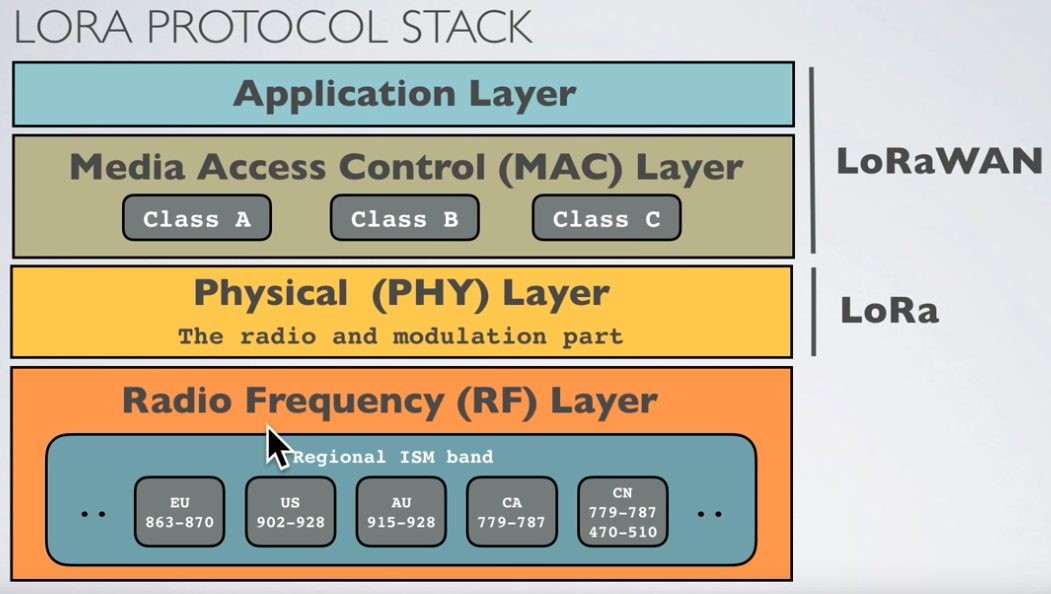
\includegraphics[width=1\linewidth]{images/capitulo2/lora_stack.png}
	\caption{\centering Pila de protocolo LoRa \cite{lora_stack}.}
	\label{fig:lora_stack}
\end{figure}

La pila del protocolo LoRa , tal y como se muestra en la Figura \ref{fig:lora_stack} se divide en varias capas. En la base se encuentra la capa de frecuencia de radio (RF), que define las bandas regionales ISM utilizadas para la transmisión (como las bandas de 863-870 MHz en Europa y 902-928 MHz en EE.UU.). Encima está la capa física (PHY), que se encarga de la radio y la modulación de la señal. La capa de control de acceso al medio (MAC) incluye las clases A, B y C, que definen diferentes modos de transmisión y recepción, ajustando el consumo de energía. En la parte superior está la capa de aplicación, que interactúa directamente con los servicios y aplicaciones de los usuarios. LoRaWAN abarca la capa MAC y la capa de aplicación.

\begin{figure}[H]
	\centering
	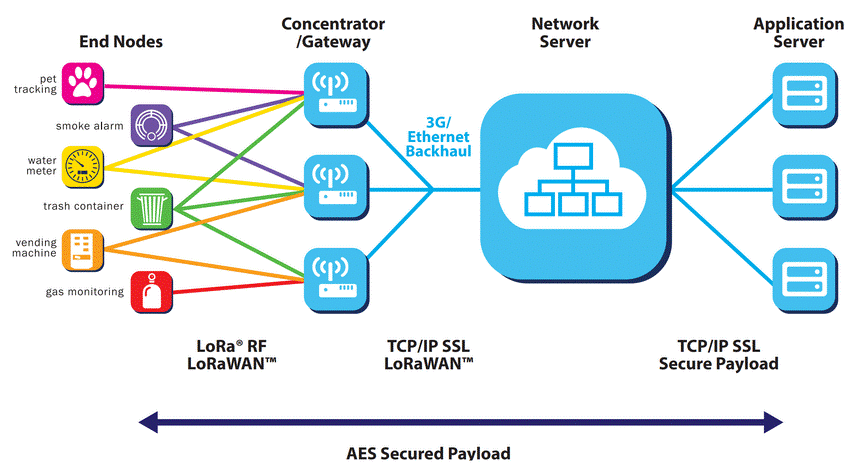
\includegraphics[width=1\linewidth]{images/capitulo2/lora_arq.png}
	\caption{\centering Arquitectura de una red LoRaWAN enfocada en nodos finales múltiples \cite{lora_alliance}.}
	\label{fig:lora_arq}
\end{figure}

\begin{figure}[H]
	\centering
	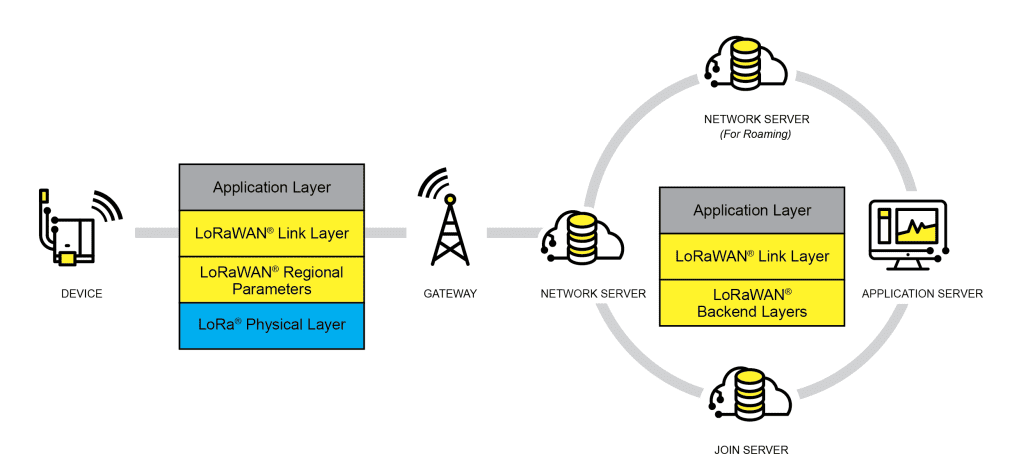
\includegraphics[width=1\linewidth]{images/capitulo2/lorawan_arq.png}
	\caption{\centering Arquitectura de una red LoraWAN enfocada en servidores múltiples \cite{lora_alliance}.}
	\label{fig:lorawan_arq}
\end{figure}

El funcionamiento de LoRaWAN en una red de dispositivos conectados como se muestra en la Figuras \ref{fig:lora_arq} y \ref{fig:lorawan_arq}. Un dispositivo envía datos a través de una gateway, que luego los transmite a un servidor de red. El servidor de red, a su vez, se comunica con los servidores de aplicaciones y servidores de registro (join server), que gestionan el acceso y almacenamiento de los datos. La imagen destaca cómo las capas del protocolo (física, parámetros regionales, y de enlace) se usan para garantizar la comunicación eficiente entre los diferentes elementos de la red.

\section{Descripción de componentes utilizados para el nodo sensor de CO\(_2\)}

A continuación se muestran los componentes electrónicos requeridos para un nodo sensor o nodo final (end node), tal y como se muestra en la Figura \ref{fig: estructura_general_IoT}. Estos nodos recopilan información de su entorno mediante sensores, tranmitirla o recibir instrucciones del gateway, por lo que mantienen una comunicación bidireccional.

\begin{figure}[H]
	\centering
	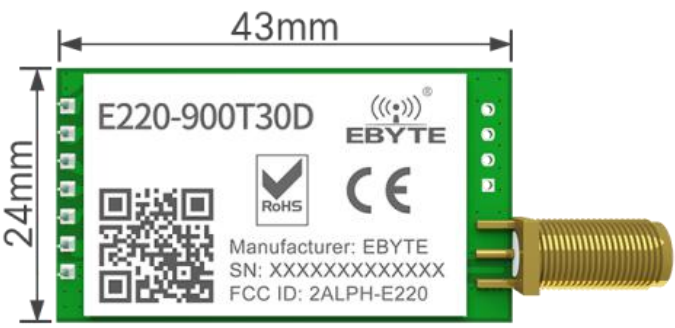
\includegraphics[width=0.65\linewidth]{images/capitulo2/modulo_lora.png}
	\caption{\centering Módulo LoRa E220-900T30D \cite{modulo_lora}.}
	\label{fig:modulo_lora}
\end{figure}

El módulo E220-900T30D, mostrado en la Figura \ref{fig:modulo_lora}, es un dispositivo que utiliza tecnología LoRa para comunicación en la banda de 868/915 MHz, basado en el chip LLCC68. Ofrece una transmisión eficiente a largas distancias, alcanzando hasta 10 km en condiciones óptimas, y presenta una alta capacidad de resistencia a interferencias. Admite diferentes modos de operación, incluyendo transmisión fija y por difusión, además de contar con funciones de monitoreo y activación por aire, lo que lo hace ideal para aplicaciones que requieren bajo consumo de energía. Este módulo puede funcionar con voltajes de 3.0 a 5.5V, siendo compatible con niveles de 3.3V y 5V en sus interfaces UART. Con un consumo mínimo en modo de suspensión (alrededor de 5 $\mu$A), es adecuado para aplicaciones como automatización del hogar, sistemas de seguridad y control remoto en entornos industriales, soportando temperaturas extremas de $-40$ a $+85$ °C.



\begin{figure}[H]
	\centering
	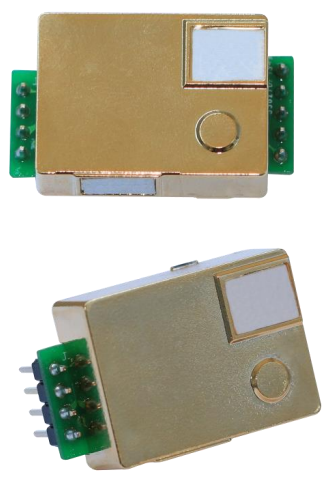
\includegraphics[width=0.65\linewidth]{images/capitulo2/sensor_co2.png}
	\caption{\centering Sensor de CO\(_2\) MH-Z19B \cite{sensor_co2}.}
	\label{fig:sensor_co2}
\end{figure}

El sensor MH-Z19B es un módulo infrarrojo no dispersivo (NDIR: non dispersive infrared detector) que permite detectar CO\(_2\) en el aire de manera precisa y estable. Su diseño compacto y de bajo consumo incluye compensación de temperatura, lo que lo hace adecuado para aplicaciones como la monitorización de calidad del aire en interiores, sistemas de climatización (HVAC: heating, ventilation and air conditioning) y dispositivos inteligentes. Ofrece múltiples opciones de salida de datos, incluyendo UART y PWM, y es capaz de medir concentraciones de CO\(_2\) en un rango de 0 a 2000 ppm o hasta 5000 ppm, con un tiempo de respuesta inferior a 120 segundos y una vida útil superior a los 5 años.




\begin{figure}[H]
	\centering
	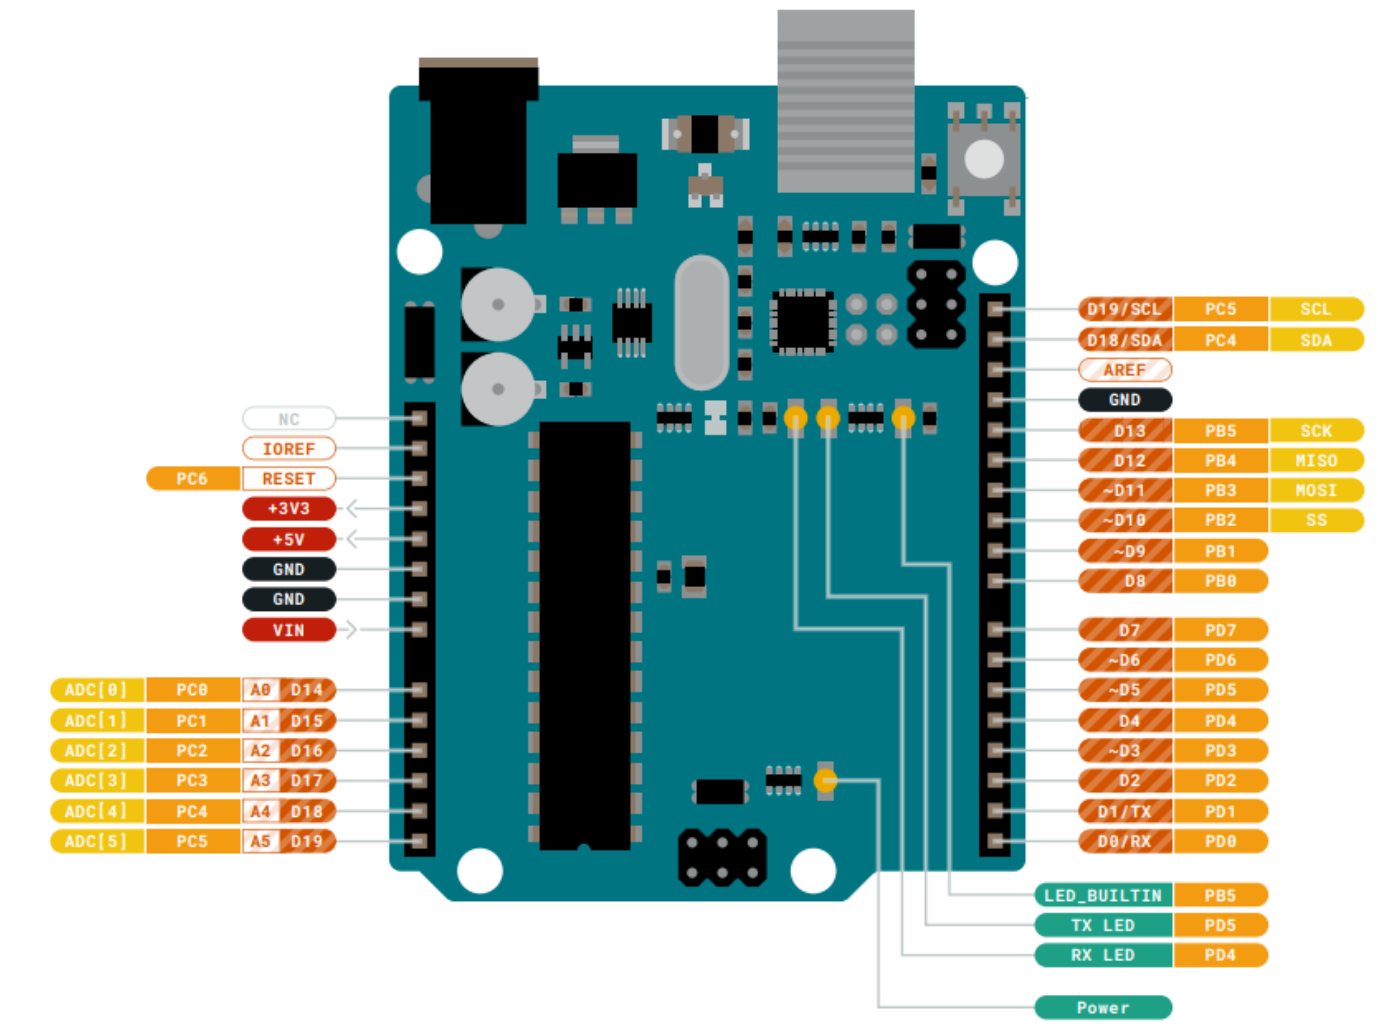
\includegraphics[width=0.65\linewidth]{images/capitulo2/arduino_uno_pins_datasheet.png}
	\caption{\centering Sensor de CO\(_2\) \cite{arduino_uno_datasheet}.}
	\label{fig:arduino}
\end{figure}

El microcontrolador ATMEGA328P, el cual es utilizado en la placa Arduino UNO mostrada en la Figura \ref{fig:arduino}, está basado en una arquitectura AVR de 8 bits y opera a una frecuencia máxima de 16 MHz. Ofrece una memoria Flash de 32 KB, 2 KB de SRAM y 1 KB de EEPROM, junto con múltiples interfaces de comunicación, como UART, SPI e I2C. Además, cuenta con un convertidor ADC de 10 bits y varios temporizadores, lo que lo hace adecuado para aplicaciones de control y monitoreo. Funciona en un rango de voltaje de 1.8 a 5.5 V y admite modos de bajo consumo, como Power-save, Standby y Power-down, lo que lo convierte en una excelente opción para proyectos de electrónica educativa y aplicaciones embebidas que no requieren altas velocidades de procesamiento \cite{arduino_uno_datasheet}.








\section{Amazon Web Services (AWS)}
Amazon Web Services (AWS) es una plataforma de computación en la nube proporcionada por Amazon, que ofrece una extensa variedad de servicios bajo demanda, como almacenamiento, bases de datos, capacidad de cómputo y soluciones de redes. Funciona a través de una infraestructura global de centros de datos, lo que permite a los usuarios acceder a recursos de manera flexible y pagar un monto variable en función a los recursos utilizados. AWS facilita a empresas y desarrolladores el despliegue y escalado rápido de aplicaciones sin la necesidad de invertir en infraestructura física. Se emplea principalmente para alojar aplicaciones web, manejar grandes volúmenes de datos y ejecutar análisis en tiempo real, ayudando a optimizar costos y recursos operativos.


\section{SQL Server Management Studio}
SQL Server Management Studio (SSMS) es una herramienta de administración para trabajar con instancias de bases de datos SQL Server, tanto en instalaciones locales como en la nube. Permite gestionar servidores y bases de datos mediante una interfaz gráfica intuitiva, facilitando la creación de consultas, gestión de objetos de base de datos, monitoreo de rendimiento y ejecución de scripts. Funciona integrando herramientas avanzadas para desarrolladores y administradores de bases de datos, simplificando tareas como la configuración de servidores, monitoreo y análisis de consultas \cite{sql_server}.



\section{.NET Core}
.NET es una plataforma de desarrollo multiplataforma y de código abierto que permite crear aplicaciones en una variedad de lenguajes, como C\# y Visual Basic. Funciona ofreciendo un entorno de ejecución eficiente, herramientas avanzadas, y un conjunto de bibliotecas para crear aplicaciones de escritorio, móviles, web y servicios en la nube. .NET permite a los desarrolladores construir soluciones escalables y de alto rendimiento, tanto para entornos locales como en la nube, y es ideal para proyectos modernos que requieren flexibilidad y compatibilidad multiplataforma \cite{net_core}.






\chapter{MARCO METODOLÓGICO}

El trabajo de investigación se divide en los siguientes tres frentes: nodo sensor, aplicación web y gateway. En este sentido, se ha optado por dividir la metodología para tener una mejor documentación del proceso a seguir en cada frente del proyecto, tanto en la selección de los componentes electrónicos empleados y los protocolos de comunicación inalámbrica más eficientes, así como de las tecnologías empleadas para la selección.

\begin{itemize}
    \item \textbf{Desarrollo de nodo sensor}
    \item \textbf{Desarrollo de la aplicación web}
    \item \textbf{Configuración del gateway}
    \item \textbf{Desarrollo del subsistema de mitigación activa y control}
\end{itemize}

\section{Metodologías de investigación}

\subsection{Metodología V model}
Para el desarrollo de la aplicación web, se ha escogido la metodología V model. Esta metodología permite estructurar y gestionar de manera eficaz el proceso de desarrollo y prueba, asegurando que cada fase de construcción esté alineada con un proceso de validación correspondiente. A continuación se describe la adaptación de este modelo al desarrollo de la aplicación web de monitoreo de datos de CO\(_2\).

\begin{figure}[H]
    \centering
    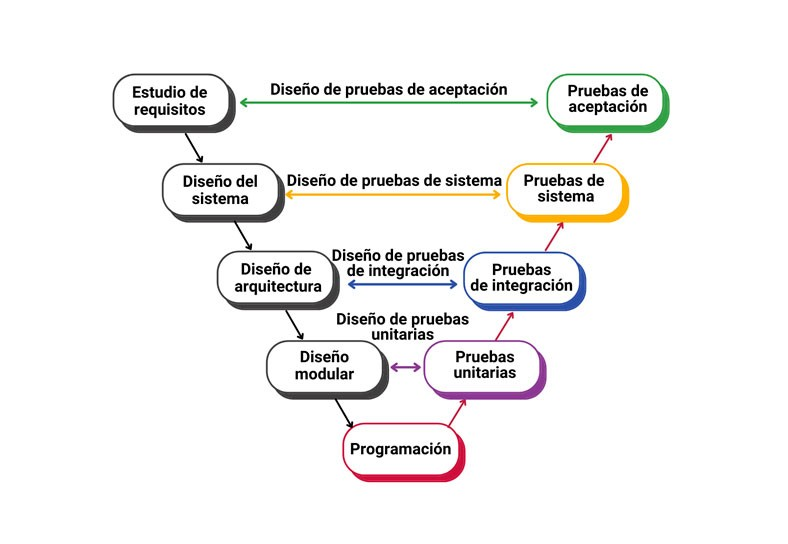
\includegraphics[width=0.9\linewidth]{images/capitulo3/vmodel.png}
    \caption{\centering Metodología V model \cite{vmodel}.}
    \label{fig:vmodel}
\end{figure}



\subsubsection{Definición de Requisitos}

En esta primera etapa, se establecen los requisitos funcionales y no funcionales de la aplicación web. Estos incluyen la capacidad para recibir y mostrar los datos provenientes del mega gateway Kona, almacenar y consultar dichos datos en una base de datos SQL, y activar alertas visuales y sonoras cuando los niveles de CO\(_2\) superen un umbral predeterminado.

\subsubsection{Diseño de Sistema y Arquitectura}

En esta fase, se desarrolla una arquitectura que permita la integración de todos los componentes necesarios para la recepción, almacenamiento y visualización de los datos. Se emplea la arquitectura por capas, la cual a su vez considera el uso de un backend basado en C\# y .NET, una API para la comunicación entre el backend y el frontend, y un frontend en React, con TypeScript y empleando la librería Tailwind para el diseño visual, optimizado para una visualización de los datos recopilados por los nodos sensores.

\subsubsection{Diseño de Componentes}

Aquí se realiza el diseño específico de cada componente de la aplicación web, considerando el flujo de datos entre el mega gateway Kona, la base de datos y la interfaz de usuario. Esta fase incluye el diseño de la estructura de la base de datos SQL para almacenar las lecturas, la configuración de la API para recibir los datos del gateway mediante el protocolo MQTT, y la implementación de componentes de interfaz en React para visualizar los datos y alertas.

\subsubsection{Implementación y Codificación}

En la fase de implementación, se lleva a cabo la construcción de cada componente diseñado. El backend en .NET maneja la lógica de negocio y la comunicación con la base de datos, mientras que el frontend en React presenta los datos al usuario y envía alertas cuando los niveles de CO\(_2\) son elevados. Cada parte del código se implementa luego con pruebas unitarias y de integración para asegurar el cumplimiento de los requisitos.

\subsubsection{Verificación y Validación}

Una vez implementados los componentes, se realizan pruebas de integración y validación para asegurar que la aplicación web funcione de acuerdo con los requisitos establecidos. Esto incluye pruebas de visualización y actualización de datos en tiempo real, pruebas de respuesta de la interfaz de usuario y pruebas de activación de alertas visuales y auditivas cuando los niveles de CO\(_2\) superan los umbrales establecidos.

\subsubsection{Pruebas de Sistema}

Finalmente, se lleva a cabo una prueba de sistema que verifica la interacción completa entre los diferentes módulos y la precisión en la recepción y visualización de datos en tiempo real. En esta fase se simulan diferentes escenarios, incluyendo niveles normales y elevados de CO\(_2\), para garantizar que la aplicación web cumpla con su propósito y proporcione alertas efectivas y accesibles al usuario.

\subsubsection{Mantenimiento y Actualización}

El modelo V incluye una fase de mantenimiento, donde se abordan posibles mejoras, correcciones de errores y ajustes de la interfaz para optimizar la experiencia del usuario. Dado que la aplicación web estará en constante interacción con datos en tiempo real, es crucial que el mantenimiento se realice de forma periódica para asegurar su fiabilidad y precisión en la entrega de información y alertas.












\subsection{Metodología PPDIOO}

Para el desarrollo del nodo sensor y la configuración del gateway, se ha optado por emplear la metodología PPDIOO. Esta metodología se adapta bien a la implementación de sistemas de hardware y redes, pues permite una planificación detallada en cada fase, asegurando la fiabilidad y eficiencia del sistema desde la concepción hasta la operación y mejora continua. A continuación, se describe la aplicación de esta metodología en los dos frentes del proyecto: el nodo sensor y el gateway.

\begin{figure}[H]
    \centering
    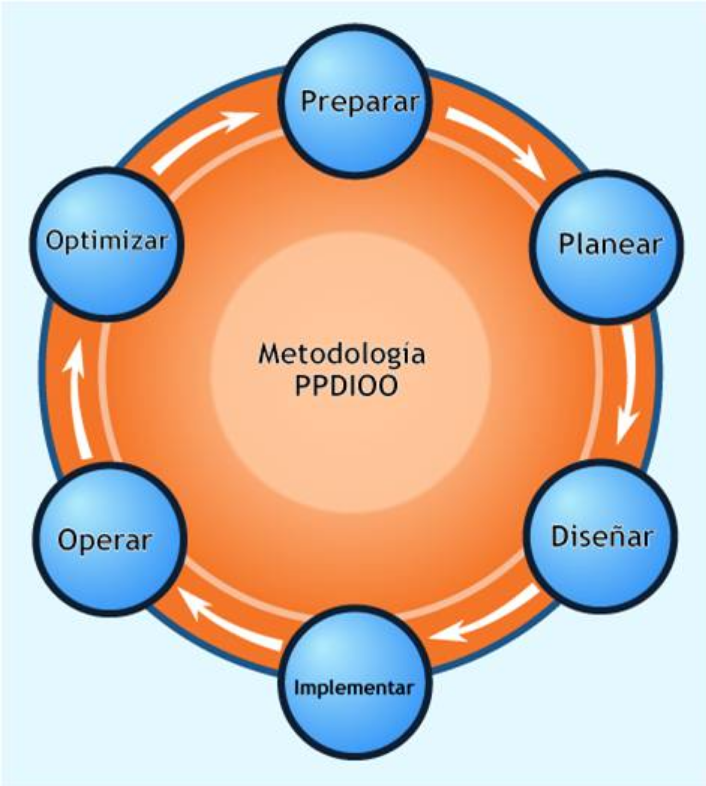
\includegraphics[width=0.5\linewidth]{images/capitulo3/PPDIOO.png}
    \caption{\centering Metodología PPDIOO \cite{PPDIOO}.}
    \label{fig:PPDIOO}
\end{figure}



\subsubsection{Planificación}

En esta fase inicial, se definen los objetivos y especificaciones del nodo sensor. Se identifican los componentes necesarios, que incluyen un sensor de CO\(_2\), un microcontrolador para el procesamiento de datos, y un módulo de comunicación LoRa para el envío de los datos al gateway. También se establecen los requisitos de transmisión, frecuencia de muestreo (configurable) y los umbrales de alerta para la detección de niveles elevados de CO\(_2\).

\subsubsection{Preparación}

Durante la preparación, se lleva a cabo la adquisición de los componentes y se realiza una evaluación de su compatibilidad y consumo energético. Se configura un entorno de desarrollo adecuado y se establecen conexiones de prueba entre el sensor y el microcontrolador, garantizando que el módulo LoRa pueda transmitir adecuadamente los datos generados por el sensor.

\subsubsection{Diseño}

El diseño abarca tanto el esquema de conexiones físicas del nodo sensor como la estructura del código que gestionará las lecturas del sensor. Aquí se diseña el algoritmo que leerá los datos de CO\(_2\), procesará y enviará las lecturas mediante LoRa. Se definen las configuraciones para asegurar una transmisión óptima de los datos y se diseñan métodos de verificación para validar los niveles de CO\(_2\) y activar la transmisión en tiempo real hacia el gateway.

\subsubsection{Implementación}

En la fase de implementación, se ensamblan los componentes electrónicos y se carga el código en el microcontrolador para la captura y transmisión de datos. Se llevan a cabo pruebas de comunicación entre el nodo y el gateway para asegurar que los datos se envían correctamente y que el módulo LoRa funciona de acuerdo con los requisitos establecidos.

\subsubsection{Operación}

Una vez implementado, el nodo sensor se coloca en condiciones de operación para la lectura continua de niveles de CO\(_2\) en el entorno. Esta fase implica una prueba prolongada del nodo para garantizar su rendimiento y la consistencia en la transmisión de datos hacia el gateway bajo diferentes condiciones ambientales.

\subsubsection{Optimización}

Finalmente, la fase de optimización contempla ajustes en la configuración de muestreo y transmisión para optimizar el consumo energético y mejorar la precisión de las lecturas. Se realizan actualizaciones en el código y en la calibración del sensor, de ser necesario, para asegurar que el nodo opere de manera estable y eficiente.


















\section{Desarrollo de la aplicación web}

\subsection{Estudio de requisitos}

\subsubsection{Interfaz de Usuario (Frontend)}

\begin{figure}[H]
    \centering
    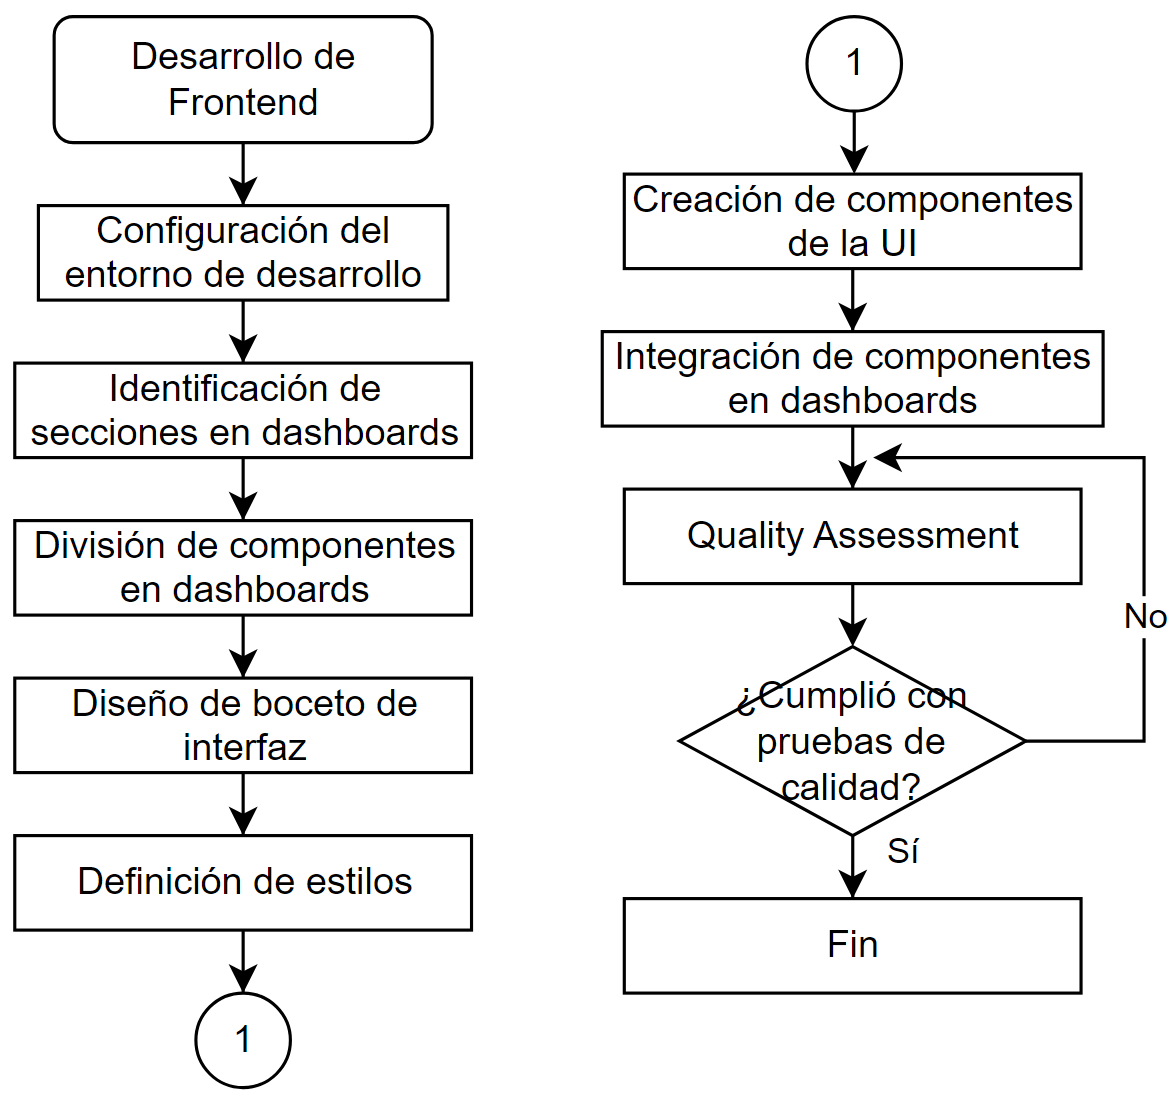
\includegraphics[width=0.6\linewidth]{images//capitulo3/DF_frontend.png}
    \caption{Diagrama de flujo para el desarrollo Frontend}
    \label{fig:DF_frontend}
\end{figure}

En la figura \ref{fig:DF_frontend} se observa la metodología seguida para del desarrollo del frontend de la aplicación web de Monitoreo. En cuanto al paso de evaluación de cualidad (QA: Quality Asessment), consiste en realizar una variedad de pruebas para asegurar el adecuado funcionamiento de la aplicación, cuyos principales focos de atención son los siguientes:

\begin{itemize}
    \item Correcciónes gramaticales.
    \item Bugs y malfuncionamientos en ciertas acciones de la aplicación.
    \item Configuraciones incompletas.
\end{itemize}


Así mismo, la página web cuenta con dos páginas que funcionan como dashboards. La primera es una landing page en la cual se detallan los datos más relevantes en la aplicaciónl, la segunda es una vista detallada para cada uno de los sensores. Las principales funciones de cada una se detallan a continuación.



\begin{itemize}
    \item \textbf{Landing page (Dashboard)}:
          \begin{itemize}
              \item Mostrar las últimas lecturas de CO\(_2\) de tres sensores en tiempo real.
              \item Incluir detalles de la ubicación de cada sensor.
              \item Visualizar las alertas cuando los valores de CO\(_2\) superen el umbral permitido (mediante ventanas emergentes y sonidos de alerta).
          \end{itemize}

    \item \textbf{Vista de Detalle de Sensor}:
          \begin{itemize}
              \item Mostrar información detallada de cada sensor, como el nombre y la ubicación.
              \item Incluir un gráfico interactivo con las lecturas de CO\(_2\) de las últimas 8 horas.
              \item Acceso desde un menú lateral que permite la navegación entre sensores.
          \end{itemize}
\end{itemize}

\subsubsection{Operaciones entre Frontend y Backend}

\begin{itemize}
    \item El frontend debe realizar solicitudes HTTP al backend para recibir actualizaciones de datos de los sensores en tiempo real.
    \item El backend enviará datos actualizados al frontend cada vez que haya una nueva lectura registrada.
    \item Cuando los datos de CO\(_2\) superen el umbral configurado, el backend enviará una señal de alerta que el frontend deberá presentar visual y sonoramente.
    \item El frontend permitirá la consulta histórica de lecturas de CO\(_2\) de cada sensor para su representación en los gráficos.
\end{itemize}

\subsubsection{Interacción con el Mega Gateway Kona}

\begin{itemize}
    \item El mega gateway Kona recibirá los datos de los sensores mediante comunicación LoRa y los enviará al backend utilizando el protocolo MQTT.
    \item El backend debe estar configurado para recibir y procesar mensajes MQTT enviados por el mega gateway Kona.
    \item Los datos recibidos desde el mega gateway Kona deben almacenarse en una base de datos SQL para su posterior visualización y consulta histórica.
    \item En caso de que el mega gateway envíe lecturas que superen el umbral, el backend debe activar el sistema de alertas.
\end{itemize}

\subsubsection{Requisitos de Almacenamiento y Persistencia de Datos}

\begin{itemize}
    \item Los datos de lectura de los sensores deben almacenarse en una base de datos SQL para permitir consultas en tiempo real y acceso a registros históricos.
    \item La base de datos debe registrar la fecha, hora, ubicación y nivel de CO\(_2\) de cada lectura.
    \item Los datos históricos deben poder ser visualizados por el usuario a través de gráficos en la interfaz de detalle de cada sensor.
\end{itemize}









\subsection{Selección de la arquitectura de software}

\begin{table}[h!]
    \centering
    \renewcommand{\arraystretch}{1.5}
    \caption{Comparación de Arquitecturas de Software para Aplicaciones de Monitoreo IoT \cite{software_arquitectura}}
    \label{tabla:software_arquitecturas}
    \begin{tabular}{|p{3cm}|p{2.5cm}|p{2.8cm}|p{2.5cm}|p{3cm}|}
        \hline
        \textbf{Arquitectura}   & \textbf{Escalabilidad}                                                                          & \textbf{Facilidad de Implementación}                                                           & \textbf{Manejo de Datos en Tiempo Real}                                                                & \textbf{Capacidad de Procesamiento}                                                                        \\ \hline
        \textbf{Por capas}      & Moderada: adecuada para aplicaciones pequeñas y medianas                                        & Alta: diseño claro y comúnmente usado en frameworks como ASP.NET y Django                      & Limitada: requiere de modificaciones para soporte en tiempo real                                       & Distribución de lógica de negocio en el backend; buena para procesamiento en servidor                      \\ \hline
        \textbf{Microservicios} & Muy alta: ideal para aplicaciones grandes y escalables, permite añadir servicios independientes & Moderada: requiere experiencia en la gestión de múltiples servicios, comunicación y despliegue & Muy buena: servicios independientes pueden manejar eventos en tiempo real                              & Procesamiento distribuido: cada servicio maneja una funcionalidad específica, óptimo para alto rendimiento \\ \hline
        \textbf{Serverless}     & Alta: escalabilidad automática y flexible, óptima para aplicaciones con carga variable          & Alta: simplifica la implementación al no requerir gestión de servidores                        & Buena: respuesta en tiempo real gestionada por eventos; adecuado para procesamiento en base a umbrales & Limitada al evento y tiempo de ejecución; más eficiente para tareas eventuales o de corta duración         \\ \hline
    \end{tabular}
\end{table}

Se decidió que la arquitectura por capas es ideal para este trabajo de investigación, dado su enfoque accesible, escalable y educativo, adecuado para el monitoreo IoT, ya que ofrece una estructura clara y modular que facilita el aprendizaje práctico de los estudiantes de cada componente en el desarrollo web. La separación en Modelo, Vista y Controlador permite a los estudiantes entender el flujo de datos desde la captura de los sensores hasta la visualización en tiempo real, y aprender de manera segmentada las responsabilidades de cada capa.

Además, la arquitectura por capas es escalable para aplicaciones de mediana complejidad, por lo que, a medida que el proyecto crezca (añadiendo sensores o funciones adicionales), podrá expandirse sin una reestructuración significativa. Su compatibilidad con frameworks educativos, como ASP.NET, el cual es utilizado para este trabajo, facilita la implementación y permite que los estudiantes se enfoquen en la lógica de negocio y el diseño de la interfaz sin la complejidad de arquitecturas más avanzadas.
\FloatBarrier






\subsection{Desarrollo del Frontend}

\subsubsection{Selección de tecnologías de diseño}
\begin{table}[h!]
    \centering
    \renewcommand{\arraystretch}{1.5}
    \caption{Comparación de Tecnologías Frontend para Aplicaciones de Monitoreo IoT}
    \label{tabla:comparativa}
    \begin{tabular}{|p{2.1cm}|p{2cm}|p{2.5cm}|p{2.5cm}|p{2.5cm}|p{3.7cm}|}
        \hline
        \textbf{Tecnología}        & \textbf{Facilidad de Uso}                   & \textbf{Rendimiento}                                          & \textbf{Soporte de Componentes de Visualización}         & \textbf{Escalabilidad}                                & \textbf{Enfoque}                                                                                                              \\ \hline
        \textbf{React}             & Alta: gran documentación y comunidad        & Alto, gracias a su DOM virtual optimizado                     & Amplio: compatible con bibliotecas como Chart.js y D3.js & Alta: compatible con arquitecturas modulares          & Creado para construir interfaces de usuario y gestionar el estado de aplicaciones de una sola página (SPA)                    \\ \hline
        \textbf{Vue.js}            & Muy alta: curva de aprendizaje rápida       & Moderado-Alto: buen manejo de cambios                         & Amplio: compatible con bibliotecas gráficas              & Moderado: adecuado para proyectos pequeños-medianos   & Enfoque progresivo, diseñado para ser adaptable y escalable según las necesidades del proyecto                                \\ \hline
        \textbf{Angular}           & Media: curva de aprendizaje más pronunciada & Alto: rendimiento robusto en aplicaciones grandes             & Muy amplio: incluye gráficos y componentes integrados    & Alta: ideal para proyectos grandes y escalables       & Framework completo orientado a aplicaciones empresariales de gran tamaño y aplicaciones SPA complejas                         \\ \hline
        \textbf{Svelte}            & Muy alta: sintaxis intuitiva y directa      & Muy alto: menos carga de procesamiento en tiempo de ejecución & Moderado: soporte de bibliotecas externas                & Moderado-Alto: más adecuado para aplicaciones ligeras & Diseño enfocado en la eficiencia, compila código en tiempo de desarrollo para optimizar el rendimiento en tiempo de ejecución \\ \hline
        \textbf{Blazor (para C\#)} & Media: requiere familiaridad con .NET       & Alto: ejecuta WebAssembly                                     & Moderado: integrable con bibliotecas .NET                & Alta: conveniente para aplicaciones basadas en .NET   & Orientado a la ejecución de aplicaciones .NET en el navegador usando WebAssembly                                              \\ \hline
    \end{tabular}
\end{table}
\FloatBarrier


Dado que el trabajo de investigación tiene un enfoque educativo y como objetivo principal establecer un flujo de trabajo sencillo para estudiantes, se considera que React es la opción más adecuada para la aplicación de monitoreo IoT. Esto debido a que permite la creación de componentes reutilizables, manteniendo un desarrollo ágil y modular, lo cual es prioritario para que el proyecto sea replicable y fácil de comprender en un entorno educativo, mientras que, a su vez, da margen suficiente para que los estudiantes puedan ajustar la aplicación en torno a sus necesidades específicas y explorar sus propios conceptos.







\subsubsection{Diseño de componentes}

A continuación se presentan los componentes creados e implementados en el diseño, tanto en el dashboard de la landing page, así como en la página de detalle de cada sensor, y la página de configuración del administrador. El código para estos componentes se puede visualizar en el anexo \ref{an:componentes_front}.

\begin{itemize}

    \item \texttt{Sidebar.tsx}: Menú lateral de navegación que permite acceder rápidamente a diferentes secciones de la aplicación, como el Dashboard, detalles de sensores, configuración y ayuda. Incluye iconos para mejorar la usabilidad y el diseño.

    \item \texttt{SensorOverview.tsx}: Muestra un resumen en tiempo real del estado de los sensores de CO\(_2\). Cada sensor tiene su propia tarjeta con información sobre el nivel actual de CO\(_2\), ubicación, estado (normal, elevado, crítico) y última actualización.

    \item \texttt{ComparativeChart.tsx}: Componente que muestra una gráfica comparativa de los niveles de CO\(_2\) de varios sensores a lo largo del tiempo. Permite visualizar las tendencias de CO\(_2\) para cada sensor y ayuda a identificar patrones o picos.

    \item \texttt{Filters.tsx}: Card que permite seleccionar el período de tiempo (última hora, últimas 3 horas, etc.) para filtrar los datos que se muestran en la gráfica comparativa (\texttt{ComparativeChart}). Incluye un selector desplegable para ajustar el rango de tiempo.

    \item \texttt{Statistics.tsx}: Card que muestra las estadísticas generales de los sensores, como el nivel promedio de CO\(_2\), el máximo alcanzado, el tiempo total en alerta y el número de alertas generadas. Está diseñado para adaptarse a la altura de su contenido y optimizar el uso del espacio.

    \item \texttt{AlertHistory.tsx}: Card que muestra un historial de alertas, con información sobre la hora de cada alerta y el nivel de CO\(_2\) registrado. Ayuda a rastrear incidentes pasados y evaluar la frecuencia de las alertas.

    \item \texttt{Alerts.tsx}: Card que muestra las alertas activas en el sistema. Cada alerta tiene información sobre la ubicación, el nivel de CO\(_2\) y el estado (elevado, crítico). Incluye botones de acción (como "Reconocer" y "Silenciar") para gestionar las alertas.

    \item \texttt{CampusMap.tsx} (Opcional): Muestra un mapa del campus con las ubicaciones de los sensores de CO\(_2\) resaltadas. Este componente fue eliminado en la última versión del Dashboard para liberar espacio, pero puede reinsertarse según sea necesario.
\end{itemize}











\subsection{Desarrollo del back end}

\subsubsection{Selección de patrones de diseño}


\begin{landscape}
    \begin{table}[h!]
        \centering
        \renewcommand{\arraystretch}{1.2} % Ajusta la altura de las filas
        \fontsize{9}{10}\selectfont % Reduce aún más el tamaño de la fuente dentro de la tabla
        \caption{Patrones de Diseño Utilizados en el Proyecto \cite{design_patterns} \cite{design_patterns}}
        \label{tabla:patrones-diseno}
        \begin{tabular}{|p{2cm}|p{3cm}|p{3cm}|p{5cm}|p{2cm}|}
            \hline
            \textbf{Patrón de Diseño}                                                                                                                                                      & \textbf{Descripción} & \textbf{Función en el Proyecto} & \textbf{Beneficios} & \textbf{Capa(s) de la Arquitectura} \\ \hline

            \textbf{DTO (Data Transfer Object)}                                                                                                                                            &
            Objeto simple que encapsula datos para transferir entre capas, evitando exponer directamente las entidades del dominio.                                                        &
            Facilita la transferencia de datos de las lecturas de sensores y alertas al frontend, asegurando que solo se transmita la información necesaria.                               &
            \begin{itemize}[leftmargin=*, nosep]
                \item Reduce el acoplamiento entre capas.
                \item Mejora la seguridad al no exponer entidades internas.
                \item Optimiza el rendimiento al transferir solo datos esenciales.
            \end{itemize}                                                                                                         &
            Capa de Aplicación $\leftrightarrow$ Capa de Presentación                                                                                                                                                                                                                                           \\ \hline

            \textbf{Repository Pattern}                                                                                                                                                    &
            Abstracción que maneja las operaciones de acceso a datos, proporcionando una interfaz para realizar operaciones CRUD.                                                          &
            Gestiona la interacción con la base de datos para almacenar y recuperar lecturas de sensores, así como verificar umbrales para generar alertas.                                &
            \begin{itemize}[leftmargin=*, nosep]
                \item Aísla la lógica de acceso a datos de la lógica de negocio.
                \item Facilita la prueba y mantenimiento del código.
                \item Permite cambiar el proveedor de datos sin afectar otras capas.
            \end{itemize}                                                                                                       &
            Capa de Persistencia                                                                                                                                                                                                                                                                                \\ \hline

            \textbf{Entity Framework (ORM)}                                                                                                                                                &
            Herramienta de mapeo objeto-relacional que permite interactuar con la base de datos utilizando modelos de entidad en lugar de consultas SQL directas.                          &
            Simplifica la gestión de la base de datos, permitiendo mapear las lecturas de sensores y alertas a entidades de C\#.                                                           &
            \begin{itemize}[leftmargin=*, nosep]
                \item Reduce la complejidad del acceso a datos.
                \item Facilita la gestión de cambios en el esquema de la base de datos.
                \item Mejora la productividad al eliminar la necesidad de escribir consultas SQL manualmente.
            \end{itemize}                                                                              &
            Capa de Persistencia                                                                                                                                                                                                                                                                                \\ \hline

            \textbf{Service Pattern}                                                                                                                                                       &
            Organiza la lógica de negocio en servicios independientes y reutilizables que encapsulan operaciones específicas.                                                              &
            Centraliza la lógica de procesamiento de datos de sensores, evaluación de umbrales y generación de alertas, manteniendo la lógica de negocio separada de otras preocupaciones. &
            \begin{itemize}[leftmargin=*, nosep]
                \item Promueve la reutilización de código.
                \item Mejora la mantenibilidad y escalabilidad del sistema.
                \item Facilita la implementación de pruebas unitarias.
            \end{itemize}                                                                                                                &
            Capa de Aplicación                                                                                                                                                                                                                                                                                  \\ \hline
        \end{tabular}
    \end{table}
    \FloatBarrier % Evita que las tablas floten por encima de este punto
\end{landscape}
\FloatBarrier














\subsubsection{Desarrollo de REST API}
\begin{figure}
    \centering
    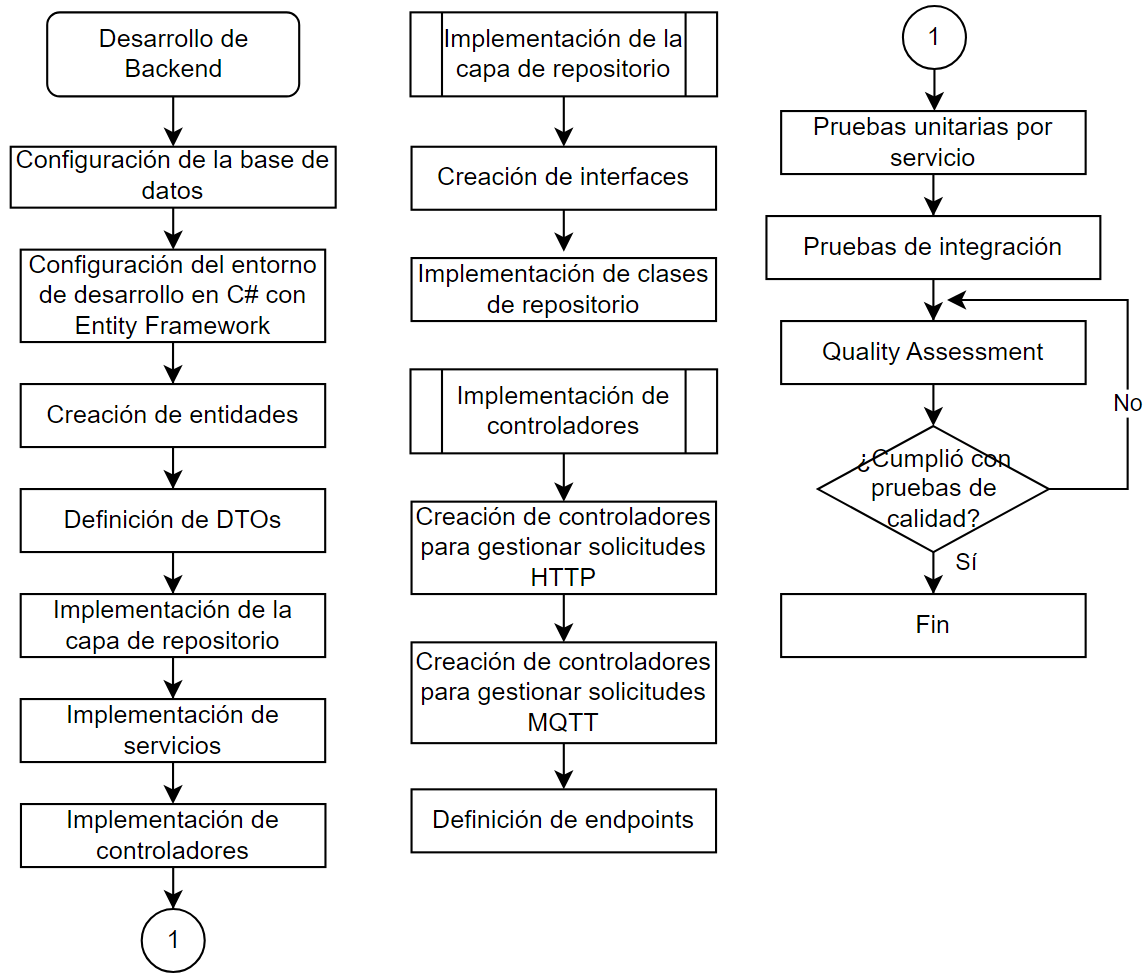
\includegraphics[width=0.8\linewidth]{images/capitulo3/DF_backend.png}
    \caption{Diagrama de flujo del desarrollo de Backend.}
    \label{fig:df_backend}
\end{figure}


El desarrollo backend sigue una arquitectura de capas en la que cada sección tiene un rol específico para gestionar las operaciones de datos de los sensores. La configuración inicial incluye la base de datos y el entorno en C\# con Entity Framework, permitiendo un acceso simplificado a MySQL mediante mapeo de objetos.

Las entidades representan las tablas en la base de datos, y los DTOs permiten transferir datos de forma controlada entre capas, protegiendo la estructura de la base de datos. La capa de repositorio usa el \textit{Repository Pattern} para manejar las operaciones \textit{CRUD} de manera aislada. La capa de servicios aplica la lógica de negocio, como verificar los umbrales de CO\(_2\) y gestionar alertas. Finalmente, los controladores gestionan las solicitudes \texttt{HTTP} y \texttt{MQTT}, proporcionando los datos al frontend mediante endpoints bien definidos.

Las pruebas unitarias e integración aseguran la calidad y funcionamiento del sistema antes del despliegue. El proceso de Quality Assessment verifica que todos los componentes cumplen con los estándares de calidad antes de finalizar el desarrollo.



\section{Desarrollo del nodo sensor}

\subsection{Selección de la tecnología de comunicación}

Antes de definir los componentes electrónicos específicos del nodo sensor, es fundamental seleccionar la tecnología de comunicación inalámbrica que mejor se adapte a los requerimientos del proyecto. En la Tabla \ref{tabla:comparativa_comunicacion} se presenta una comparativa entre las principales tecnologías IoT disponibles en el mercado, evaluadas según los criterios de diseño específicos de esta investigación.

\begin{landscape}
    \begin{table}[h!]
        \centering
        \renewcommand{\arraystretch}{1.3}
        \fontsize{9}{10}\selectfont
        \caption{Comparación de Tecnologías de Comunicación Inalámbrica para Nodos Sensores}
        \label{tabla:comparativa_comunicacion}
        \begin{tabular}{|p{2.5cm}|p{2.5cm}|p{2cm}|p{2cm}|p{2.5cm}|p{2.5cm}|p{4.5cm}|p{2cm}|}
            \hline
            \textbf{Característica}     & \textbf{LoRa}                & \textbf{Zigbee}           & \textbf{Wi-Fi}           & \textbf{Bluetooth (BLE)}        & \textbf{NB-IoT / LTE-M (Celular IoT)} & \textbf{Criterio de Diseño (Lo que busca tu Proyecto)}                                                            & \textbf{Mejor Opción}                       \\ \hline
            \textbf{Frecuencia}         & Sub-GHz (915 MHz en Perú)    & 2.4 GHz                   & 2.4 GHz y 5 GHz          & 2.4 GHz                         & Bandas Licenciadas LTE                & Se busca una frecuencia libre (ISM) y legal en Perú, preferiblemente Sub-GHz para evitar interferencia en 2.4GHz. & LoRa (915 MHz)                              \\ \hline
            \textbf{Alcance (Urbano)}   & Alto (1--5 km con obstáculos) & Bajo (10--100 m)           & Bajo (30--100 m)         & Muy Bajo ($<$10 m)                & Muy Alto ($>$5 km)                          & Se busca cubrir múltiples laboratorios en un campus universitario con un solo gateway central.                    & LoRa / Wi-Fi (ya se cuenta con repetidores) \\ \hline
            \textbf{Consumo Energía}    & Muy Bajo ($\sim$40 mA TX, pero ciclo de trabajo $<$1\%) & Bajo ($\sim$30 mA TX, pero mayor overhead en red mesh) & Alto ($\sim$200 mA TX, conexión constante $>$1 mA) & Muy Bajo ($<$15 mA TX, ráfagas muy cortas) & Medio ($\sim$200 mA TX, pero usa PSM de $\sim$3 $\mu$A)                            & Se busca que los nodos sensores puedan funcionar con baterías durante meses sin mantenimiento.                    & LoRa / BLE                                  \\ \hline
            \textbf{Tasa de Datos}      & Muy Baja (0.3--50 kbps)          & Baja (250 kbps)           & Muy Alta ($>$50 Mbps)      & Media (1--2 Mbps)                & Baja ($<$250 kbps)                            & Se busca enviar solo unos pocos bytes (valor de CO$_2$) cada varios minutos.                                      & LoRa                                        \\ \hline
            \textbf{Penetración Muros}  & Muy Alta (Link Budget $\sim$157 dB) & Baja ($\sim$104 dB) & Baja ($\sim$100 dB) & Muy Baja ($\sim$90 dB) & Muy Alta ($\sim$164 dB) & Se busca atravesar muros de concreto armado densos típicos de laboratorios y aulas.                               & LoRa / NB-IoT                               \\ \hline
            \textbf{Costo del Nodo}     & Medio (\$5--\$15)              & Muy Bajo (\$3--\$10)           & Muy Bajo (\$3--\$8)       & Muy Bajo (\$2--\$5)              & Alto (\$15--\$30)                     & Se busca minimizar el costo por nodo sensor para un despliegue de tesis.                                          & Wi-Fi / BLE                                 \\ \hline
            \textbf{¿Necesita Gateway?} & Sí                           & Sí                        & No (Router directo)      & No (Directo a móvil/PC)         & No (Base celular)                     & -                                                                                                                 & LoRa                                        \\ \hline
            \textbf{Costos Operativos}  & Muy Bajos (Nulos, red propia) & Muy Bajos (Nulos, red propia) & Muy Bajos (Nulos, red U) & Muy Bajos (Nulos)               & Altos (Suscripción mensual)           & Se busca un costo mensual cero por tráfico de datos para sostenibilidad.                                          & LoRa / Wi-Fi / Zigbee                       \\ \hline
        \end{tabular}
    \end{table}
\end{landscape}
\FloatBarrier

De acuerdo con el análisis presentado en la Tabla \ref{tabla:comparativa_comunicacion}, la tecnología \textbf{LoRa} destaca como la solución más viable y que mejor cumple con los criterios de diseño del proyecto. Su alcance en zonas urbanas (clasificado como Alto) permite conectar múltiples laboratorios en el campus utilizando un solo gateway, y su muy alta capacidad de penetración de muros resulta indispensable en infraestructuras con concreto armado. Además, opera en la banda libre de 915 MHz, idónea en Perú para evitar la congestión típica de la banda de 2.4 GHz. Un factor decisivo es su muy bajo consumo energético general; aunque su corriente pico de transmisión es comparable a la de tecnologías como Zigbee, la arquitectura de red en estrella de LoRa permite que los nodos sensores permanezcan en reposo profundo la mayor parte del tiempo (ciclo de trabajo inferior al 1\%), evitando el constante enrutamiento de datos y el alto overhead característicos de las redes en malla (mesh). Sumado a sus costos operativos muy bajos (prácticamente nulos al ser red propia), LoRa se convierte en la opción ideal para un despliegue sostenible a largo plazo, a pesar de su muy baja tasa de datos, la cual es suficiente para transmitir lecturas esporádicas de CO$_2$.

\subsection{Gateways comerciales frente a la implementación de gateways personalizados}

Para el despliegue de redes LoRaWAN enfocadas en Internet de las Cosas (IoT), la literatura resalta tres enfoques principales para la capa de borde (Edge): gateways comerciales de grado operador, gateways comerciales de bajo costo (prosumer) y gateways personalizados construidos a medida (Do-It-Yourself o DIY).

Los \textbf{gateways comerciales de grado operador (Carrier-Grade)}, como el Kona Mega Gateway, representan el estándar de infraestructura masiva. Cuentan con multiplexación avanzada para manejar entre 64 y 72 canales simultáneos, erradicando virtualmente las colisiones en el aire \cite{nb_gateway_commercial_1}, y poseen filtros físicos que logran sensibilidades excepcionales de -142 dBm \cite{nb_gateway_commercial_4}. Sin embargo, sus elevados costos (CAPEX) y la inflexibilidad de su ecosistema cerrado los hacen inviables e incompatibles con arquitecturas atípicas requeridas en proyectos universitarios de pequeña escala \cite{nb_gateway_commercial_6, nb_gateway_commercial_7}.

Por otro lado, los \textbf{gateways comerciales de bajo costo (Prosumer)}, como el RAK7268V2 o SenseCAP M2, buscan democratizar el acceso con costos entre \$89 y \$500 USD \cite{nb_gateway_commercial_6}. Integran criptografía robusta en hardware (ATECC608A) y procesadores digitales de señal (DSP) \cite{nb_gateway_prosumer_29}. A pesar de estos beneficios, su limitación a 8 canales físicos genera riesgos de congestión, forzando la dependencia de mecanismos como la Tasa de Datos Adaptativa (ADR) \cite{nb_gateway_prosumer_32, nb_gateway_prosumer_34}, además de incurrir en costos ocultos de importación y periféricos adicionales \cite{nb_gateway_prosumer_41}.

Finalmente, los \textbf{gateways personalizados (Custom/DIY)} se ensamblan acoplando microcontroladores o computadoras de placa única (SBC) a módulos concentradores LoRa o transceptores \cite{nb_gateway_custom_9}. Este enfoque ofrece flexibilidad absoluta de software y control total sobre las rutinas de enrutamiento \cite{nb_gateway_custom_7}. Su principal virtud es la posibilidad de operar en modo ``promiscuo'', lo que permite interactuar con nodos de ultra bajo costo que carecen de la pila LoRaWAN completa, además de reducir dramáticamente el presupuesto de implementación \cite{nb_gateway_custom_10}. Si bien presentan riesgos asociados a la alta complejidad técnica y soporte fragmentado, estos desafíos son coherentes y deseables en el marco de una investigación de tesis en Ingeniería Mecatrónica, donde se busca precisamente el dominio de la integración hardware-software a bajo nivel.

En conclusión, para este proyecto universitario desarrollado en Lima, Perú, se determina la viabilidad técnica y académica de optar por el diseño e implementación de un \textbf{gateway personalizado}. La priorización de la flexibilidad para configurar nodos simples, la reducción contundente del CAPEX y la alineación con los objetivos de diseño embebido respaldan sólidamente esta decisión frente al sobredimensionamiento y rigidez de los equipos comerciales. Esta elección fundamenta, a su vez, la necesidad de una evaluación exhaustiva de microcontroladores y módulos de comunicación para el ensamble tanto del nodo sensor como del gateway.

\subsection{Selección de componentes}

Para determinar los elementos electrónicos y de comunicación que compondrán tanto los nodos sensores como el gateway personalizado, se evalúan las principales alternativas reportadas en la literatura. Dado que el proyecto requiere viabilidad para un prototipado realista y replicable en el entorno universitario (Lima, Perú), se han ajustado los criterios de evaluación otorgando un peso preponderante del 35\% a la ``Disponibilidad en el mercado local'' y 30\% a la ``Facilidad de configuración / Abundancia de documentación''. A continuación, se presentan las matrices de evaluación para microcontroladores, módulos LoRa y módulos Wi-Fi.

\subsubsection{Evaluación de Microcontroladores}

Se evaluaron cuatro opciones predominantes:
\begin{itemize}
    \item \textbf{MCU 1: ATmega328P.} Microcontrolador base de Arduino UNO. Su severa limitación de memoria SRAM provoca inestabilidad al intentar implementar una pila LoRaWAN completa \cite{nb_mcu_1, nb_mcu_3}.
    \item \textbf{MCU 2: ESP32.} Microcontrolador de muy bajo costo con conectividad Wi-Fi nativa, altamente versátil para nodos sensores austeros y tareas de enrutamiento en gateways minimalistas \cite{nb_mcu_4, nb_mcu_6}.
    \item \textbf{MCU 3: ESP32-S3.} Variante de doble núcleo, utilizada en gateways comerciales de bajo costo para compilar lógicas de reenvío digital \cite{nb_mcu_6}.
    \item \textbf{MCU 4: Microchip ATECC608A.} Coprocesador criptográfico utilizado para cifrado de hardware, pero que no actúa como unidad de procesamiento general \cite{nb_mcu_8}.
\end{itemize}

\begin{table}[H]
    \centering
    \renewcommand{\arraystretch}{1.5}
    \caption{Evaluación Comparativa de Microcontroladores}
    \label{tabla:evaluacion_mcu}
    \begin{tabular}{|p{4.5cm}|p{1.5cm}|p{1.5cm}|p{1.5cm}|p{1.5cm}|p{1.5cm}|}
        \hline
        \textbf{Criterio de Evaluación} & \textbf{Peso} & \textbf{MCU 1} & \textbf{MCU 2} & \textbf{MCU 3} & \textbf{MCU 4} \\ \hline
        Disponibilidad local & 35\% & 4 (1.40) & 4 (1.40) & 2 (0.70) & 1 (0.35) \\ \hline
        Facilidad de configuración & 30\% & 4 (1.20) & 4 (1.20) & 3 (0.90) & 2 (0.60) \\ \hline
        Capacidad de procesamiento/RAM & 20\% & 1 (0.20) & 3 (0.60) & 4 (0.80) & 2 (0.40) \\ \hline
        Costo & 15\% & 3 (0.45) & 4 (0.60) & 3 (0.45) & 2 (0.30) \\ \hline
        \textbf{Puntaje Total} & \textbf{100\%} & \textbf{3.25} & \textbf{3.80} & \textbf{2.85} & \textbf{1.65} \\ \hline
    \end{tabular}
\end{table}

\subsubsection{Evaluación de Módulos LoRa}

Las alternativas para la capa física de radiofrecuencia (transceptores/concentradores) incluyen:
\begin{itemize}
    \item \textbf{LoRa 1: Ebyte E220-900T30D.} Transceptor UART de bajo costo basado en el chip LLCC68, ideal para nodos y gateways monocanal simples, aunque requiere que la estructura de red sea gestionada por software \cite{nb_lora_1}.
    \item \textbf{LoRa 2: RAKwireless RAK2287.} Módulo concentrador impulsado por el chip SX1302 con escudo EMI, excelente para gateways multicanal robustos \cite{nb_lora_13}.
    \item \textbf{LoRa 3: Seeed Studio Wio-WM1302.} Tarjeta concentradora SX1302 con certificaciones industriales, optimizada en consumo y costo \cite{nb_lora_13_seeed}.
    \item \textbf{LoRa 4: Dragino PG1302.} Módulo tipo Pi HAT orientado a presupuestos ajustados, pero con soporte técnico limitado \cite{nb_lora_13_dragino}.
\end{itemize}

\begin{table}[H]
    \centering
    \renewcommand{\arraystretch}{1.5}
    \caption{Evaluación Comparativa de Módulos LoRa}
    \label{tabla:evaluacion_lora}
    \begin{tabular}{|p{4.5cm}|p{1.5cm}|p{1.5cm}|p{1.5cm}|p{1.5cm}|p{1.5cm}|}
        \hline
        \textbf{Criterio de Evaluación} & \textbf{Peso} & \textbf{LoRa 1} & \textbf{LoRa 2} & \textbf{LoRa 3} & \textbf{LoRa 4} \\ \hline
        Disponibilidad local & 35\% & 4 (1.40) & 1 (0.35) & 1 (0.35) & 2 (0.70) \\ \hline
        Facilidad de configuración & 30\% & 4 (1.20) & 3 (0.90) & 3 (0.90) & 2 (0.60) \\ \hline
        Capacidad multicanal / SNR & 20\% & 2 (0.40) & 4 (0.80) & 4 (0.80) & 3 (0.60) \\ \hline
        Costo & 15\% & 4 (0.60) & 2 (0.30) & 3 (0.45) & 3 (0.45) \\ \hline
        \textbf{Puntaje Total} & \textbf{100\%} & \textbf{3.60} & \textbf{2.35} & \textbf{2.50} & \textbf{2.35} \\ \hline
    \end{tabular}
\end{table}

\subsubsection{Evaluación de Módulos Wi-Fi}

Para la transmisión del lado del gateway o nodos que cuenten con enlace directo al servidor:
\begin{itemize}
    \item \textbf{Wi-Fi 1: Módulo Wi-Fi 4 Estándar (802.11 b/g/n).} Componente externo genérico presente en gateways comerciales, idóneo para 2.4 GHz y entornos urbanos \cite{nb_wifi_16}.
    \item \textbf{Wi-Fi 2: Wi-Fi Nativo ESP32.} Circuitería embebida en el encapsulado del microcontrolador ESP32. Provee un puente directo e ininterrumpido al enrutador sin requerir hardware físico adicional \cite{nb_mcu_4, nb_mcu_6}.
    \item \textbf{Wi-Fi 3: Wi-Fi 5 de Orange Pi Zero 3.} Módulo embebido en la SBC, con alta conectividad para arquitecturas de Edge Computing.
    \item \textbf{Wi-Fi 4: Wi-Fi 5 de Raspberry Pi 4.} Integración inalámbrica de alta velocidad apta para albergar bases de datos locales complejas.
\end{itemize}

\begin{table}[H]
    \centering
    \renewcommand{\arraystretch}{1.5}
    \caption{Evaluación Comparativa de Soluciones Wi-Fi}
    \label{tabla:evaluacion_wifi}
    \begin{tabular}{|p{4.5cm}|p{1.5cm}|p{1.5cm}|p{1.5cm}|p{1.5cm}|p{1.5cm}|}
        \hline
        \textbf{Criterio de Evaluación} & \textbf{Peso} & \textbf{Wi-Fi 1} & \textbf{Wi-Fi 2} & \textbf{Wi-Fi 3} & \textbf{Wi-Fi 4} \\ \hline
        Disponibilidad local & 35\% & 3 (1.05) & 4 (1.40) & 2 (0.70) & 3 (1.05) \\ \hline
        Facilidad de configuración & 30\% & 3 (0.90) & 4 (1.20) & 3 (0.90) & 4 (1.20) \\ \hline
        Ancho de banda & 20\% & 3 (0.60) & 2 (0.40) & 4 (0.80) & 4 (0.80) \\ \hline
        Integración y tamaño & 15\% & 2 (0.30) & 4 (0.60) & 3 (0.45) & 2 (0.30) \\ \hline
        \textbf{Puntaje Total} & \textbf{100\%} & \textbf{2.85} & \textbf{3.60} & \textbf{2.85} & \textbf{3.35} \\ \hline
    \end{tabular}
\end{table}

\subsubsection{Justificación Cualitativa de Resultados}

Con base en la evaluación de los tres dominios presentados, la selección final converge de manera natural y transparente hacia el ecosistema del \textbf{ESP32 (MCU 2 y Wi-Fi 2)} en conjunto con el \textbf{módulo Ebyte E220-900T30D (LoRa 1)}.

Debido a que el proyecto se contextualiza como un desarrollo universitario en Lima y se ha priorizado el modelo de diseño "Custom/DIY", la ponderación asignada a la "Disponibilidad en el mercado local" y la "Facilidad de configuración" ha sido decisiva. El ESP32 lidera sólidamente frente a alternativas limitadas como el ATmega328P o escasas como el ESP32-S3, brindando memoria holgada para gestionar las rutinas de transmisión e integrando sin costo adicional ni ocupación de espacio físico una interfaz Wi-Fi completamente funcional.

Por otro lado, aunque los concentradores multicanal basados en el SX1302 (como el RAK2287) presentan un puntaje técnico superior en capacidad de radio, su nula disponibilidad en el mercado local, sus altos aranceles de importación y su exigente curva de aprendizaje penalizan severamente su puntaje final. En contraste, el módulo E220-900T30D (915 MHz) domina el mercado nacional peruano de prototipado, resulta extremadamente accesible y es plenamente compatible con el ESP32 mediante su interfaz serial UART. Esta sinergia ESP32 + E220-900T30D permite construir nodos y un gateway base altamente viables, respaldados por una inmensa comunidad técnica que garantiza el cumplimiento de los objetivos de la tesis.

\subsection{Criterios Normativos para la Ubicación Espacial de los Nodos Sensores}

Para garantizar la fiabilidad y representatividad de las mediciones de dióxido de carbono (CO$_2$) en espacios universitarios, como laboratorios y aulas, es imperativo fundamentar la instalación física de los nodos sensores en normativas y estándares internacionales reconocidos. Un posicionamiento incorrecto puede derivar en lecturas sesgadas o la aparición de puntos ciegos. A partir de la revisión de literatura, se detallan los siguientes criterios estandarizados adoptados para este proyecto:

\subsubsection{Altura de Colocación Respecto a la Zona de Respiración}
Las normativas convergen en que los sensores deben situarse de manera que capturen el aire en la ``zona de respiración'' típica de los ocupantes. El estándar \textit{RESET} y el estándar \textit{WELL} recomiendan el montaje vertical en paredes a una altura comprendida entre 1.1 y 1.7 metros (o de 900 a 1800 mm) desde el nivel del suelo \cite{reset_standard_v2, well_performance_guidebook}. Por su parte, la normativa ASHRAE 62.1-2022 define esta zona de respiración en un rango similar, desde 75 hasta 1800 mm de altura \cite{ashrae_62_1_2022}. En el contexto específico de entornos educativos y de cuidado infantil, el gobierno británico aconseja de forma práctica posicionar los sensores a la altura de las mesas o de las cabezas de los estudiantes cuando se encuentran sentados \cite{gov_uk_ventilation_education}. 

\subsubsection{Distancia Mínima a Fuentes de Ventilación y Aperturas}
La proximidad a flujos de aire directo puede alterar las mediciones reales del ambiente, generando subestimaciones del riesgo. En este sentido, el estándar \textit{RESET} indica una separación mínima de 5 metros respecto a ventanas operables, filtros y difusores de aire fresco \cite{reset_standard_v2}. En caso de que el espacio sea demasiado pequeño, el sensor no debe instalarse a una distancia menor a la mitad del ancho de la habitación respecto a las ventanas. Asimismo, normativas como \textit{WELL} y \textit{RESET} dictaminan un alejamiento mínimo de 1 metro de puertas interiores, ventanas, sistemas mecánicos de suministro de aire y cualquier fuente significativa de calor o frío \cite{well_performance_guidebook, reset_standard_v2}. En el caso de puertas que den al exterior, se requieren precauciones adicionales, debiendo mantener una separación de 3 a 5 metros para evitar corrientes de aire irregulares al abrirse \cite{well_performance_guidebook}. El gobierno británico también es explícito en este punto, recomendando alejar los sensores de salidas de ventilación \cite{gov_uk_ventilation_education}.

\subsubsection{Posicionamiento Estratégico y Representatividad Espacial}
Para que las lecturas sean útiles en un sistema de mitigación, los monitores deben estar instalados de manera representativa. \textit{RESET} exige que se ubiquen centralmente en el espacio \cite{reset_standard_v2}. Además, para evitar lecturas distorsionadas causadas por la exhalación directa de una persona, el gobierno británico aconseja colocar los sensores a una distancia de al menos 0.5 metros de cualquier ocupante \cite{gov_uk_ventilation_education}. Como regla general para aulas escolares típicas, un único sensor ubicado según estas directrices es suficiente para obtener medidas precisas de la sala completa \cite{gov_uk_ventilation_education}. En casos de ambientes más amplios y diáfanos, \textit{WELL} permite utilizar un solo monitor por cada 2500 metros cuadrados si existen evidencias de un volumen de aire bien mezclado sin puntos ciegos \cite{well_performance_guidebook}. De forma excepcional, \textit{WELL} habilita la instalación horizontal en techos solo si su altura es inferior a 3.7 metros y se demuestra una mezcla homogénea de aire \cite{well_performance_guidebook}, sin embargo, el enfoque central en la zona de respiración montada en pared es el más apropiado para las aulas universitarias del proyecto.


\subsubsection{Definición de Parámetros de Instalación}
Con base en las normativas expuestas, se ha consolidado un conjunto de reglas precisas para la instalación física de los nodos sensores en los espacios evaluados de la universidad. Estos parámetros buscan un equilibrio entre el cumplimiento de los estándares internacionales (ASHRAE, RESET, WELL) y las particularidades arquitectónicas de las aulas universitarias, garantizando mediciones consistentes y libres de sesgos. En la Tabla \ref{tabla:criterios_instalacion} se resumen las recomendaciones de la literatura frente a los valores definitivos seleccionados para el despliegue de esta tesis.

\begin{table}[H]
    \centering
    \renewcommand{\arraystretch}{1.5}
    \caption{Selección de Criterios para la Instalación de Nodos Sensores de CO$_2$}
    \label{tabla:criterios_instalacion}
    \begin{tabular}{|p{4cm}|p{5.5cm}|p{4.5cm}|}
        \hline
        \textbf{Criterio de Instalación} & \textbf{Recomendación de la Literatura} & \textbf{Valor Seleccionado para el Proyecto} \\ \hline
        Altura de colocación & 1.1 a 1.7 m (RESET, WELL); 0.75 a 1.8 m (ASHRAE); Altura de cabeza sentado (GOV.UK) & \textbf{1.2 metros} (Altura promedio de respiración de estudiantes sentados) \\ \hline
        Distancia a fuentes de aire directo (ventanas, difusores) & 5 m ideal, o mínimo mitad del ancho de la habitación (RESET) & \textbf{$\geq$ 2.5 metros} (Adaptado al tamaño de las aulas universitarias) \\ \hline
        Distancia a puertas y ventanas cerradas & Mínimo 1 m (WELL, RESET) & \textbf{1.5 metros} \\ \hline
        Distancia a puertas exteriores & 3 a 5 metros (WELL) & \textbf{$\geq$ 4 metros} \\ \hline
        Distancia a ocupantes & Mínimo 0.5 metros (GOV.UK) & \textbf{1 metro} de separación del escritorio más cercano \\ \hline
        Posicionamiento espacial & Central en la habitación (RESET) o en techo si H $<$ 3.7 m y aire mixto (WELL) & \textbf{Pared central}, sin interferencias u obstáculos directos \\ \hline
    \end{tabular}
\end{table}

La justificación de los valores definidos en la Tabla \ref{tabla:criterios_instalacion} responde directamente a la dinámica del flujo de aire y al comportamiento habitual en las aulas. Al seleccionar una altura de 1.2 metros, se asegura que las lecturas reflejen de manera precisa la concentración de dióxido de carbono que los estudiantes están inhalando mientras permanecen sentados durante las clases teóricas, evitando la recolección de aire estancado a nivel del suelo o bolsas de calor cerca del techo. Por otro lado, establecer distancias mínimas estrictas frente a ventanas operables (2.5 metros) y puertas (1.5 metros) previene que corrientes puntuales de aire fresco diluyan artificialmente las mediciones, lo que podría retrasar la activación del sistema de mitigación predictiva. Finalmente, mantener una distancia prudente de 1 metro respecto a los estudiantes y centralizar los sensores en las paredes laterales permite evaluar el estado volumétrico real de la masa de aire del aula, garantizando una caracterización homogénea y confiable del entorno evaluado.

\newpage
\section{Configuración del gateway}
Para la configuración del gateway Kona Mega, primero se debe confirmar que tanto la computadora, desde donde se enviará la configuración, y el gateway estén en la misma red. Se pueden emplear 2 herramientas. Por un lado, se tiene la opción de utilizar una consola para comunicarse con el dispositivo via SSH (Secure Shell). Esto puede realizarse ya sea en el sistema operativo (OS: Operative System) Linux, el cual cuenta con una consola SSH preinstalada, así como una serie de comandos que pueden agilizar la interacción con el gateway durante la configuración; o también se pueden utilizar aplicaciones como PuTTY para la comunicación via SSH. Por otro lado, se puede emplear la aplicacion Kona Field Tool (KonaFT), la cual fue la empleada en este proyecto. Esta herramienta no solo permite realizar las configuraciones del gateway mediante una interfaz gráfica de usuario (GUI: Graphic User Interface), sino también, identificar la dirección IP de todos los dispositivos TekTelic conectados a la misma red que la computadora en la que está instalada el programa. El proceso de idetificación y configuración del gateway sigue el siguiente flujo mostrado en la figura \ref{fig:DF_gateway}.


\begin{figure}
    \centering
    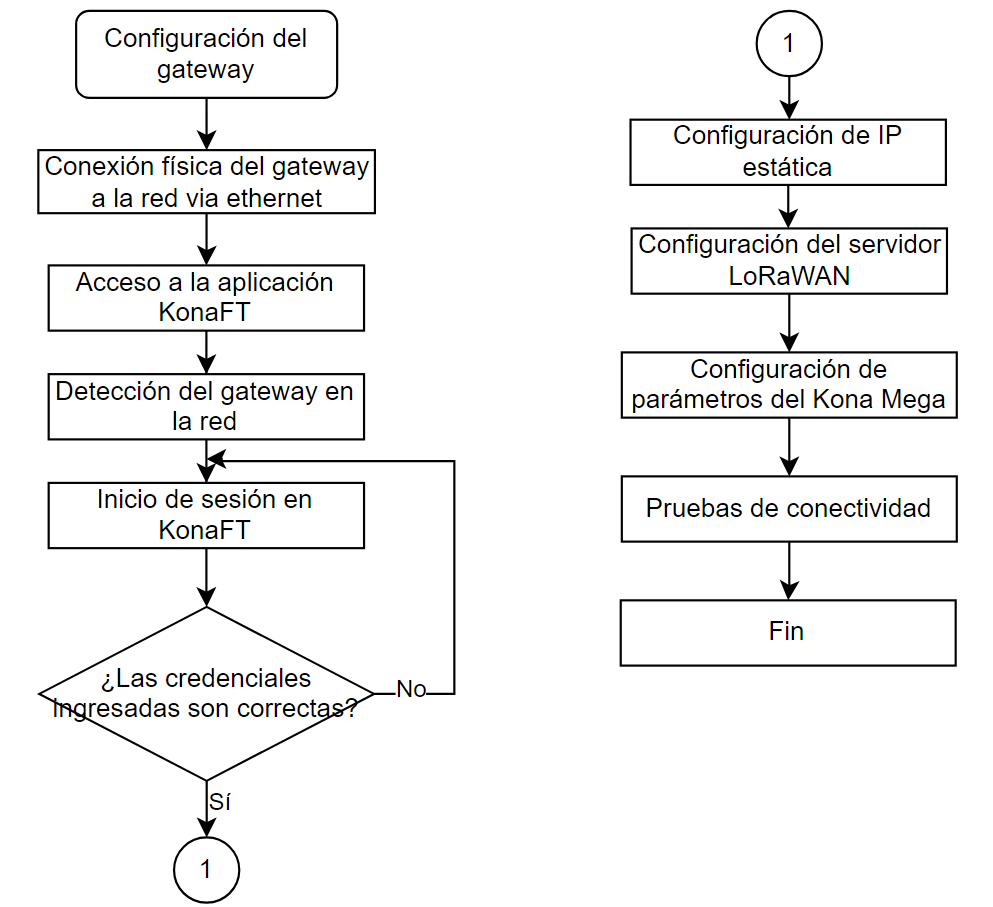
\includegraphics[width=0.8\linewidth]{images/capitulo3/DF_gateway.png}
    \caption{Diagrama de flujo de la configuración del gateway Kona Mega.}
    \label{fig:DF_gateway}
\end{figure}




\newpage
\section{Desarrollo del subsistema de mitigación activa y control}
En esta sección se presenta el desarrollo del subsistema de mitigación activa y control, incorporado con el propósito de extender la funcionalidad del sistema más allá del monitoreo pasivo de la concentración de CO$_2$. Este subsistema se basa en la actuación automática de ventiladores modulados por PWM, de modo que la ventilación del ambiente pueda ajustarse de acuerdo con las condiciones medidas en tiempo real. Para ello, se considera la definición de requisitos del subsistema, la selección de actuadores y fuente de alimentación, el diseño de la arquitectura de control, el modelado del comportamiento dinámico del CO$_2$ en ambientes interiores y la implementación de controladores PID y Fuzzy. Finalmente, se establecen los criterios de validación experimental para comparar ambas estrategias y determinar su conveniencia dentro del sistema propuesto.




\subsection{Definición de requisitos del subsistema de ventilación}

En esta etapa se establecen los requisitos funcionales y no funcionales del subsistema de ventilación activa, cuyo propósito es contribuir a la reducción de la concentración de CO$_2$ en ambientes interiores a partir de la información proporcionada por el sistema de monitoreo. Para ello, el subsistema debe ser capaz de recibir como entrada la concentración de CO$_2$ medida en tiempo real, compararla con un valor de referencia establecido y generar una acción de control que permita regular la velocidad de los ventiladores mediante señal PWM. Asimismo, el subsistema debe integrarse con la arquitectura general del proyecto, de modo que la etapa de sensado, procesamiento, actuación y visualización funcione de manera coordinada.

Desde el punto de vista funcional, se requiere que el sistema permita la activación automática de la ventilación cuando la concentración de CO$_2$ supere el nivel de referencia definido, así como la modulación de la velocidad de los ventiladores de acuerdo con la estrategia de control implementada. De igual manera, debe registrar variables relevantes para el análisis experimental, tales como la concentración medida, el error respecto al setpoint y la señal de control aplicada. Adicionalmente, el diseño debe permitir la implementación y comparación de distintas estrategias de control, específicamente PID y Fuzzy, a fin de evaluar su desempeño en términos de rapidez de respuesta, estabilidad y capacidad de mitigación.

En cuanto a los requisitos no funcionales, el subsistema debe emplear componentes comerciales de fácil adquisición e integración, operar de forma estable y segura, y ser compatible con las condiciones de infraestructura disponibles en el entorno universitario de implementación. Asimismo, debe mantener una complejidad adecuada para el desarrollo de un prototipo experimental de tesis, permitiendo su validación en escenarios controlados y su posible escalabilidad hacia implementaciones futuras de mayor alcance.


\begin{itemize}
    \item Recepción en tiempo real de la concentración de CO$_2$ medida por el sistema de sensado.
    \item Definición de un valor de referencia o setpoint para la concentración de CO$_2$.
    \item Activación automática del sistema de ventilación cuando se superen los niveles establecidos.
    \item Modulación de velocidad de los ventiladores mediante señal PWM.
    \item Implementación y comparación de controladores PID y Fuzzy.
    \item Registro de variables relevantes para validación experimental.
    \item Integración con la arquitectura IoT general del sistema.
\end{itemize}



\subsection{Selección de actuadores y fuente de alimentación}

En esta subsección se evalúan las alternativas de actuadores consideradas para el subsistema de mitigación activa, así como los requerimientos de alimentación asociados a su implementación. La selección se realiza considerando criterios como compatibilidad con control PWM, caudal de aire, presión estática, consumo de corriente, facilidad de integración y disponibilidad comercial. A partir de esta comparación, se determina la alternativa más adecuada para el prototipo y la fuente de alimentación necesaria para garantizar una operación estable del sistema de ventilación.


\begin{table}[H]
    \centering
    \renewcommand{\arraystretch}{1.3}
    \caption{Comparación de alternativas de ventiladores para el subsistema de mitigación activa}
    \label{tab:comparacion_ventiladores}
    \begin{tabular}{|p{3.6cm}|p{1.4cm}|p{1.9cm}|p{1.8cm}|p{1.8cm}|p{1.8cm}|p{3.4cm}|}
        \hline
        \textbf{Modelo} & \textbf{Voltaje} & \textbf{Control} & \textbf{Caudal} & \textbf{Presión estática} & \textbf{Corriente nominal} & \textbf{Observación} \\ \hline

        Cooler Master SickleFlow 120 ARGB (MFX-B2DN-18NPA-R1) & 12 V & PWM (4 pines) & 62 CFM & 2.5 mmH$_2$O & 0.15 A & Buena integración con PWM, bajo consumo y presión estática adecuada. \\ \hline

        Cooler Master MasterFan MF120 Halo (MFL-B2DN-18NPA-R1) & 12 V & PWM (4 pines) & 47.2 CFM & 1.6 mmH$_2$O & 0.25 A & Integración sencilla, pero menor caudal y menor presión estática. \\ \hline

        Cooler Master MasterFan MF120 Lite ARGB (MFW-B2DN-17NPA-R1) & 12 V & PWM (4 pines) & 70.5 CFM & 2.0 mmH$_2$O & 0.45 A & Mayor caudal entre las opciones de 12 V, aunque con mayor consumo. \\ \hline

        Delta PFB1224UHEP0 & 24 V & PWM + Tacómetro & --- & --- & 2.00 A & Opción industrial de alto desempeño, pero con mayor requerimiento de potencia y menor conveniencia para un prototipo universitario. \\ \hline
    \end{tabular}
\end{table}


De acuerdo con la comparación realizada, las alternativas de 12 V con control PWM presentan una integración más sencilla para el prototipo experimental, debido a su compatibilidad con señales de control por microcontrolador y a la disponibilidad de fuentes comerciales accesibles. Entre ellas, el modelo SickleFlow 120 ARGB ofrece un equilibrio favorable entre caudal, presión estática, consumo y facilidad de integración, mientras que el MF120 Lite destaca por su mayor caudal, aunque a costa de un mayor consumo de corriente. Por otro lado, la alternativa Delta representa una solución de mayor exigencia eléctrica, por lo que resulta menos conveniente para la implementación del sistema propuesto a escala de tesis.




\subsection{Diseño de la arquitectura de control}

La arquitectura de control del subsistema de mitigación activa se plantea como un sistema de lazo cerrado, en el cual la variable controlada es la concentración de CO$_2$ en el ambiente interior y la variable manipulada es la velocidad de los ventiladores. El sistema recibe como entrada la concentración de CO$_2$ medida en tiempo real por el sensor, la compara con un valor de referencia o setpoint, y calcula una acción de control orientada a reducir la diferencia entre ambas señales. De esta manera, la ventilación del ambiente puede ajustarse automáticamente en función de las condiciones reales del recinto.

Desde el punto de vista funcional, la arquitectura está conformada por cuatro bloques principales: sensado, procesamiento, control y actuación. En el bloque de sensado, el sensor de CO$_2$ adquiere la concentración presente en el ambiente y envía dicha información al sistema de procesamiento. En el bloque de procesamiento, la señal medida es acondicionada y utilizada como entrada para el algoritmo de control. Posteriormente, en el bloque de control, se genera una señal de mando a partir del error entre la concentración medida y la referencia establecida. Finalmente, en el bloque de actuación, dicha señal se traduce en una modulación PWM aplicada a los ventiladores, ajustando su velocidad y, por tanto, el caudal de aire introducido o extraído del recinto.

Esta arquitectura permite implementar distintas estrategias de control sobre una misma estructura física, facilitando la comparación entre controladores PID y Fuzzy. Asimismo, el uso de una configuración de lazo cerrado permite que el sistema responda de manera automática frente a variaciones en la ocupación del ambiente o en la concentración de CO$_2$, favoreciendo una operación más estable y adaptable que un esquema de activación basado únicamente en umbrales fijos.

\subsection{Modelado de la dinámica de \texorpdfstring{CO$_2$}{CO2} en ambientes interiores}

Para el diseño del subsistema de mitigación activa, es necesario contar con un modelo que represente la evolución de la concentración de CO$_2$ en el ambiente interior a lo largo del tiempo. En este trabajo, dicha dinámica se modela a partir de un balance de masa, considerando como principales factores la generación de CO$_2$ por parte de los ocupantes, la concentración de CO$_2$ del aire exterior y la renovación de aire producida por el sistema de ventilación. Este enfoque permite describir de manera simplificada el comportamiento del contaminante dentro del recinto y constituye la base para el diseño y evaluación de las estrategias de control.

Bajo estas consideraciones, la variación temporal de la concentración de CO$_2$ puede expresarse mediante una ecuación diferencial de primer orden, en la cual la concentración interior aumenta debido a la generación asociada a la ocupación y disminuye en función del caudal de ventilación y de la diferencia entre la concentración interior y la exterior. De esta manera, el modelo permite analizar cómo distintos niveles de ocupación y diferentes velocidades de ventilación influyen en la calidad del aire interior.

La ecuación general utilizada para representar esta dinámica es la siguiente:

\begin{equation}
\frac{dC(t)}{dt} = \frac{G(t)}{V} - \frac{Q(t)}{V}\left(C(t)-C_{out}\right)
\end{equation}

donde \(C(t)\) es la concentración de CO$_2$ en el ambiente interior, \(C_{out}\) es la concentración de CO$_2$ del aire exterior, \(G(t)\) representa la tasa de generación de CO$_2$ por los ocupantes, \(Q(t)\) es el caudal de ventilación y \(V\) es el volumen del recinto. En este modelo, la variable manipulada es el caudal de ventilación, el cual depende de la velocidad de los ventiladores controlados por PWM, mientras que la variable controlada es la concentración interior de CO$_2$.

A partir de esta formulación, es posible simular distintos escenarios de operación y analizar la respuesta del sistema ante cambios en la ocupación o en las condiciones de ventilación. Asimismo, este modelo proporciona una base adecuada para la implementación y comparación de controladores PID y Fuzzy, al permitir evaluar la evolución de la concentración de CO$_2$ frente a diferentes acciones de control.


\begin{itemize}
    \item \(C(t)\): concentración de CO$_2$ en el ambiente interior.
    \item \(C_{out}\): concentración de CO$_2$ del aire exterior.
    \item \(G(t)\): tasa de generación de CO$_2$ por los ocupantes.
    \item \(Q(t)\): caudal de ventilación.
    \item \(V\): volumen del recinto.
\end{itemize}


\subsection{Diseño e implementación de controladores PID y Fuzzy}

Con el fin de evaluar distintas estrategias de mitigación activa de CO$_2$ en ambientes interiores, se planteó el diseño e implementación de dos esquemas de control sobre una misma arquitectura física: un controlador PID y un controlador Fuzzy. En ambos casos, la variable controlada corresponde a la concentración de CO$_2$ en el recinto, mientras que la variable manipulada es la velocidad de los ventiladores, regulada mediante una señal PWM. De esta forma, ambas estrategias actúan sobre el mismo sistema y bajo las mismas condiciones de operación, permitiendo una comparación directa de su desempeño.

En el caso del controlador PID, la acción de control se calcula a partir del error entre la concentración medida y el valor de referencia establecido. Este esquema combina una acción proporcional, una integral y una derivativa, con el objetivo de reducir el error en estado estacionario, mejorar la rapidez de respuesta y atenuar oscilaciones en la salida. La ley de control utilizada se expresa de la siguiente manera:

\begin{equation}
u(t) = K_p e(t) + K_i \int e(t)\,dt + K_d \frac{de(t)}{dt}
\end{equation}

donde \(e(t)\) representa el error entre la concentración medida de CO$_2$ y el setpoint definido, mientras que \(u(t)\) corresponde a la señal de control que posteriormente se traduce en un duty cycle PWM aplicado a los ventiladores. La sintonización de los parámetros \(K_p\), \(K_i\) y \(K_d\) se realiza buscando un compromiso entre rapidez de corrección, estabilidad y ausencia de sobreimpulso excesivo.

Por otro lado, el controlador Fuzzy se plantea como una alternativa basada en reglas lingüísticas, adecuada para sistemas con incertidumbre o comportamiento no lineal. En este caso, las variables de entrada consideradas son el error de concentración de CO$_2$ y la variación del error, mientras que la variable de salida corresponde al ajuste de la señal PWM aplicada al sistema de ventilación. A partir de funciones de pertenencia y una base de reglas tipo IF-THEN, el controlador determina la acción de control más conveniente según el estado del sistema, sin depender de un modelo matemático exacto del proceso.

Para la implementación de ambas estrategias, se establece una misma estructura de operación: el sensor mide la concentración de CO$_2$, el sistema calcula el error respecto al valor de referencia, el controlador correspondiente genera la acción de control y esta señal se aplica a los ventiladores mediante modulación PWM. De esta manera, tanto el controlador PID como el controlador Fuzzy pueden evaluarse bajo un mismo entorno de simulación y, posteriormente, sobre la plataforma experimental, permitiendo comparar su comportamiento en términos de tiempo de respuesta, estabilidad, capacidad de mitigación y esfuerzo de control.

En ambos casos, la implementación se orienta a determinar cuál de las dos estrategias presenta mejores resultados para la reducción de CO$_2$ en ambientes universitarios, considerando no solo la rapidez de corrección, sino también la estabilidad de la respuesta y la factibilidad de integración en un sistema de bajo costo.



\subsection{Criterios de evaluación y validación experimental}

La evaluación del subsistema de mitigación activa y control se plantea con el objetivo de comparar el desempeño de las estrategias PID y Fuzzy bajo condiciones equivalentes de operación. Para ello, ambos controladores serán analizados sobre la misma arquitectura de sensado y actuación, considerando la concentración de CO$_2$ como variable controlada y la señal PWM aplicada a los ventiladores como variable manipulada. La validación se realizará tanto en simulación como en pruebas experimentales, con el fin de observar la respuesta del sistema frente a variaciones en la concentración inicial de CO$_2$ y ante cambios en las condiciones del ambiente interior.

Los criterios principales de evaluación considerados en este trabajo son el tiempo de establecimiento, entendido como el tiempo requerido para que la concentración de CO$_2$ alcance y permanezca próxima al valor de referencia; el sobreimpulso, asociado a desviaciones excesivas respecto al setpoint; el error en estado estacionario, que permite medir la precisión de regulación del sistema; y el esfuerzo de control, representado por la intensidad de la acción aplicada a los ventiladores mediante PWM. Asimismo, se considera la estabilidad general de la respuesta y la capacidad del controlador para recuperar condiciones aceptables de calidad del aire ante perturbaciones o incrementos en la generación de CO$_2$ dentro del recinto.

A partir de estos criterios, la validación experimental permitirá determinar cuál de las dos estrategias presenta un mejor compromiso entre rapidez de respuesta, estabilidad, precisión y factibilidad de implementación en un sistema de bajo costo orientado a espacios universitarios. De esta manera, la comparación no solo se enfocará en la disminución de la concentración de CO$_2$, sino también en la viabilidad práctica de integrar cada controlador dentro del prototipo desarrollado.







\newpage
\section{Integración del sistema}

El diagrama de flujo muestra el funcionamiento general del sistema integrado. Entre los pasos mencionados, proceso como la validación y formateo de datos en el gateway antes de enviarlos a la base de datos, si bien son brevemente mencionado en el diagrama, son esenciales para asegurar integridad y evitar errores. Además, el gateway debe gestionar eficientemente la conexión MQTT para asegurar que no haya pérdida de datos durante la transmisión. Cuando se genera una alerta por niveles de CO$_2$ altos, esta no solo se envía al frontend, sino que también puede almacenarse en la base de datos para un historial.

\begin{figure}[H]
    \centering
    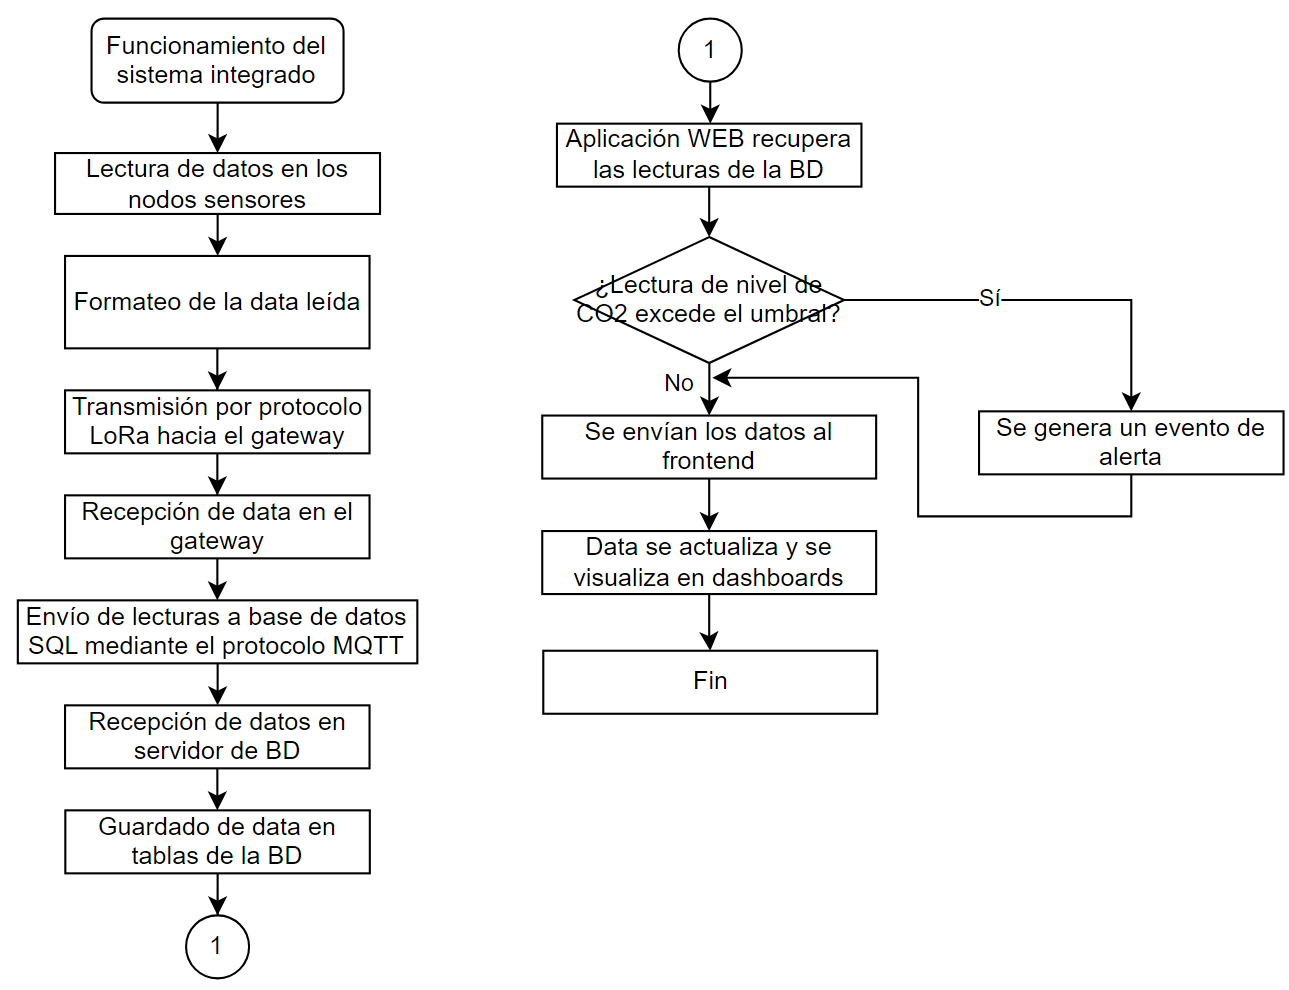
\includegraphics[width=\linewidth]{images/capitulo3/DF_integracion.png}
    \caption{Diagrama de flujo del funcionamiento del sistema}
    \label{fig:DF_integracion}
\end{figure}

\chapter{RESULTADOS}
\label{ch:resultados}

En el presente capítulo, se muestra el análisis de los resultados obtenidos a partir de la simulación e implementación de las estrategias de control desarrolladas en el marco metodológico. Se presentan las conexiones del nodo sensor, los resultados de simulación del controlador PI/PID, los resultados experimentales del controlador PI/PID y la validación de la página web para la lectura de los sensores.

\section{Conexiones del nodo sensor}

Se realizaron las conexiones entre la placa de prototipado Arduino UNO, el sensor MH-Z19B y el módulo LoRa E220-900T30D como se muestra en la figura \ref{fig:diagrama_conexiones}. Los pines utilizados para cada componente se detallan en la tabla \ref{tabla:conexiones}.




\begin{figure}[H]
    \centering
    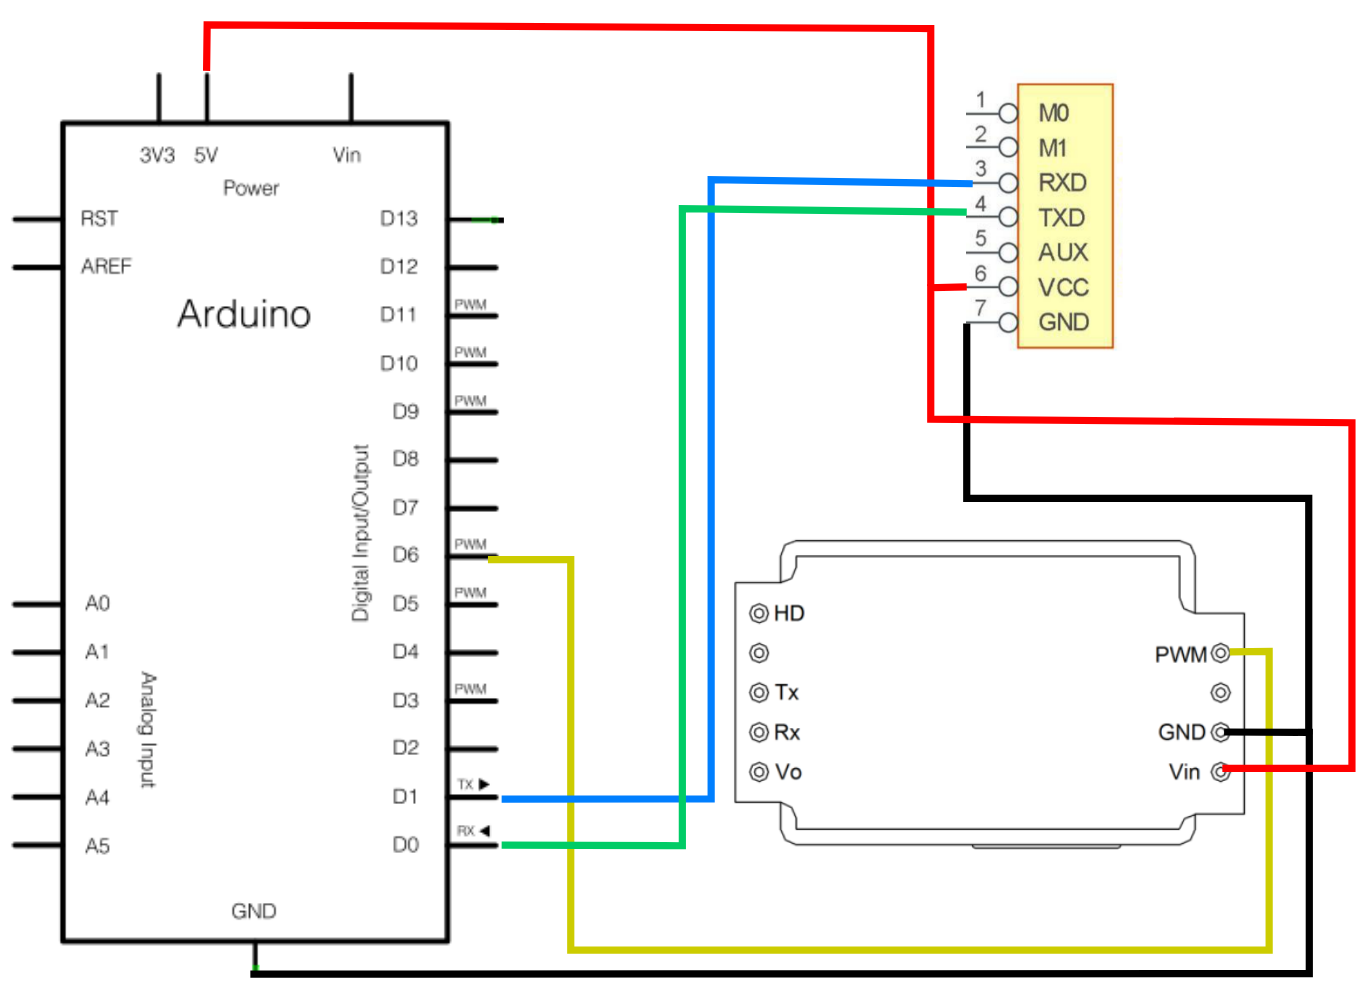
\includegraphics[width=\linewidth]{images/capitulo4/diagrama_conexiones.png}
    \caption{Diagrama de conexiones del nodo sensor}
    \label{fig:diagrama_conexiones}
\end{figure}



\begin{table}[h!]
    \centering
    \renewcommand{\arraystretch}{1.5}
    \caption{Conexiones para el nodo sensor}
    \label{tabla:conexiones}
    \begin{tabular}{|c|c|c|}
        \hline
        \textbf{Pines del Arduino UNO} & \textbf{Pines del MH-Z19B} & \textbf{Pines del E220-900T30D} \\ \hline
        GND                            & GND                        & GND                             \\ \hline
        5V                             & VCC                        & VCC                             \\ \hline
        D6                             & PWM                        & -                               \\ \hline
        RX (D0)                        & -                          & TX                              \\ \hline
        TX (D1)                        & -                          & RX                              \\ \hline
    \end{tabular}
\end{table}



\section{Resultados de simulación de los controladores}

\subsection{Resultados de simulación del controlador PI/PID}

En esta sección se presentan los resultados obtenidos mediante la simulación del controlador PI/PID aplicado al modelo de concentración de CO\(_2\) en el aula. La simulación considera una condición inicial elevada de CO\(_2\), un valor de referencia de 900 ppm y la actuación de cinco ventiladores como mecanismo de mitigación activa. Los resultados permiten analizar la evolución de la concentración de CO\(_2\), el esfuerzo de control aplicado y el caudal efectivo generado por el sistema de ventilación.

\begin{figure}[H]
    \centering
    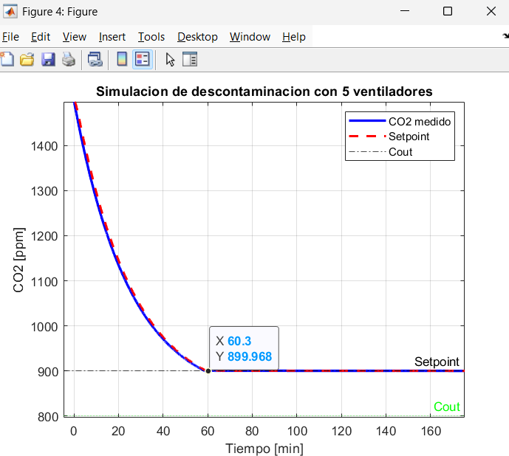
\includegraphics[width=0.9\linewidth]{images/capitulo4/PI_CO2_Simulacion.png}
    \caption{Respuesta simulada de la concentración de CO\(_2\) con controlador PI/PID.}
    \label{fig:PI_CO2_Simulacion}
\end{figure}

Como se observa en la Figura \ref{fig:PI_CO2_Simulacion}, la concentración de CO\(_2\) inicia en un valor cercano a 1500 ppm y disminuye progresivamente como consecuencia de la ventilación aplicada por el controlador. El sistema alcanza el valor de referencia de 900 ppm aproximadamente a los 60.3 minutos, con una concentración de 899.968 ppm. A partir de ese instante, la respuesta se mantiene próxima al setpoint, lo que evidencia que el controlador PI/PID permite reducir la concentración de CO\(_2\) desde una condición inicial desfavorable hasta el nivel objetivo establecido.

\begin{figure}[H]
    \centering
    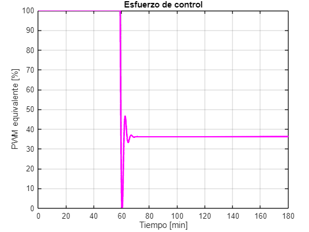
\includegraphics[width=0.9\linewidth]{images/capitulo4/PI_Esfuerzo_Simulacion.png}
    \caption{Esfuerzo de control simulado del controlador PI/PID.}
    \label{fig:PI_Esfuerzo_Simulacion}
\end{figure}

La Figura \ref{fig:PI_Esfuerzo_Simulacion} muestra el esfuerzo de control equivalente en porcentaje de PWM. Durante los primeros 60 minutos, la señal de control se mantiene cercana al 100\%, debido a que la concentración de CO\(_2\) se encuentra muy por encima del valor de referencia. Cuando el sistema alcanza la zona del setpoint, el esfuerzo de control disminuye de manera brusca y presenta una breve oscilación transitoria. Posteriormente, la señal se estabiliza alrededor de un valor aproximado de 35\% a 36\%, suficiente para mantener la concentración de CO\(_2\) cercana al valor objetivo.

\begin{figure}[H]
    \centering
    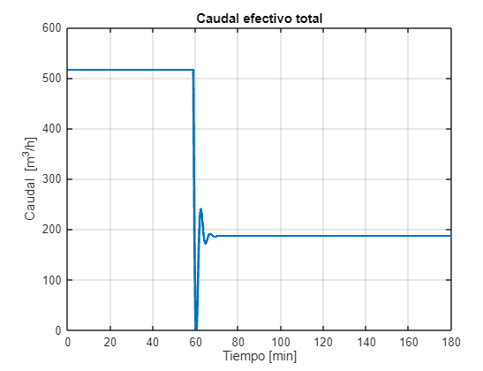
\includegraphics[width=0.9\linewidth]{images/capitulo4/PI_Caudal_Simulacion.png}
    \caption{Caudal efectivo simulado generado por el sistema de ventilación con controlador PI/PID.}
    \label{fig:PI_Caudal_Simulacion}
\end{figure}

En la Figura \ref{fig:PI_Caudal_Simulacion} se presenta el caudal efectivo total generado por el sistema de ventilación. Durante la etapa inicial, el caudal se mantiene aproximadamente en 515 m\(^3\)/h, correspondiente a una actuación máxima de los ventiladores. Alrededor de los 60 minutos, cuando la concentración de CO\(_2\) alcanza el setpoint, el caudal disminuye rápidamente y presenta un comportamiento transitorio asociado al reajuste del controlador. Finalmente, el caudal se estabiliza cerca de 185 a 190 m\(^3\)/h, lo que indica que el sistema reduce la ventilación una vez alcanzada la concentración objetivo, pero mantiene un caudal mínimo necesario para conservar el equilibrio del ambiente.

En conjunto, los resultados de simulación del controlador PI/PID muestran una respuesta estable y progresiva para la reducción de CO\(_2\). El tiempo aproximado de llegada al setpoint fue de 60.3 minutos, con una actuación máxima durante la etapa inicial y una reducción posterior del esfuerzo de control hasta un valor estacionario cercano al 35\%. Este comportamiento demuestra que el controlador PI/PID es capaz de disminuir la concentración de CO\(_2\) y ajustar la ventilación de manera progresiva, por lo que estos resultados sirven como referencia para comparar posteriormente el desempeño de las estrategias Fuzzy PI, Fuzzy PI agresiva y LQR.


\subsection{Resultados de simulación del controlador Fuzzy PI base}

En esta sección se presentan los resultados obtenidos mediante la simulación del controlador Fuzzy PI base aplicado al modelo de concentración de CO\(_2\) del aula. A diferencia del controlador PI/PID, esta estrategia emplea una base de reglas difusas para determinar el porcentaje de ventilación en función del error de concentración de CO\(_2\) y la acumulación del error. La simulación permite analizar la evolución de la concentración de CO\(_2\), el error de control, el esfuerzo de control aplicado y el caudal efectivo generado por los ventiladores.

\begin{figure}[H]
    \centering
    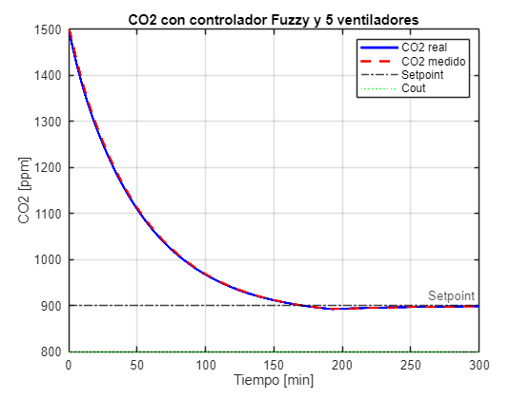
\includegraphics[width=0.9\linewidth]{images/capitulo4/FUZZY_CO2_Simulacion.png}
    \caption{Respuesta simulada de la concentración de CO\(_2\) con controlador Fuzzy PI base.}
    \label{fig:fuzzy_co2_simulacion}
\end{figure}

Como se observa en la Figura \ref{fig:fuzzy_co2_simulacion}, la concentración de CO\(_2\) inicia en un valor cercano a 1500 ppm y disminuye progresivamente debido a la acción del controlador Fuzzy PI. La respuesta presenta una reducción suave y continua, alcanzando una zona cercana al setpoint de 900 ppm aproximadamente entre los 170 y 180 minutos. Posteriormente, la concentración desciende ligeramente por debajo del valor de referencia, llegando a una zona aproximada de 890 ppm alrededor de los 190 a 210 minutos, para luego estabilizarse nuevamente cerca del setpoint. Este comportamiento muestra que el controlador Fuzzy PI logra reducir la concentración de CO\(_2\), aunque con una respuesta más lenta que la obtenida con el controlador PI/PID simulado.

\begin{figure}[H]
    \centering
    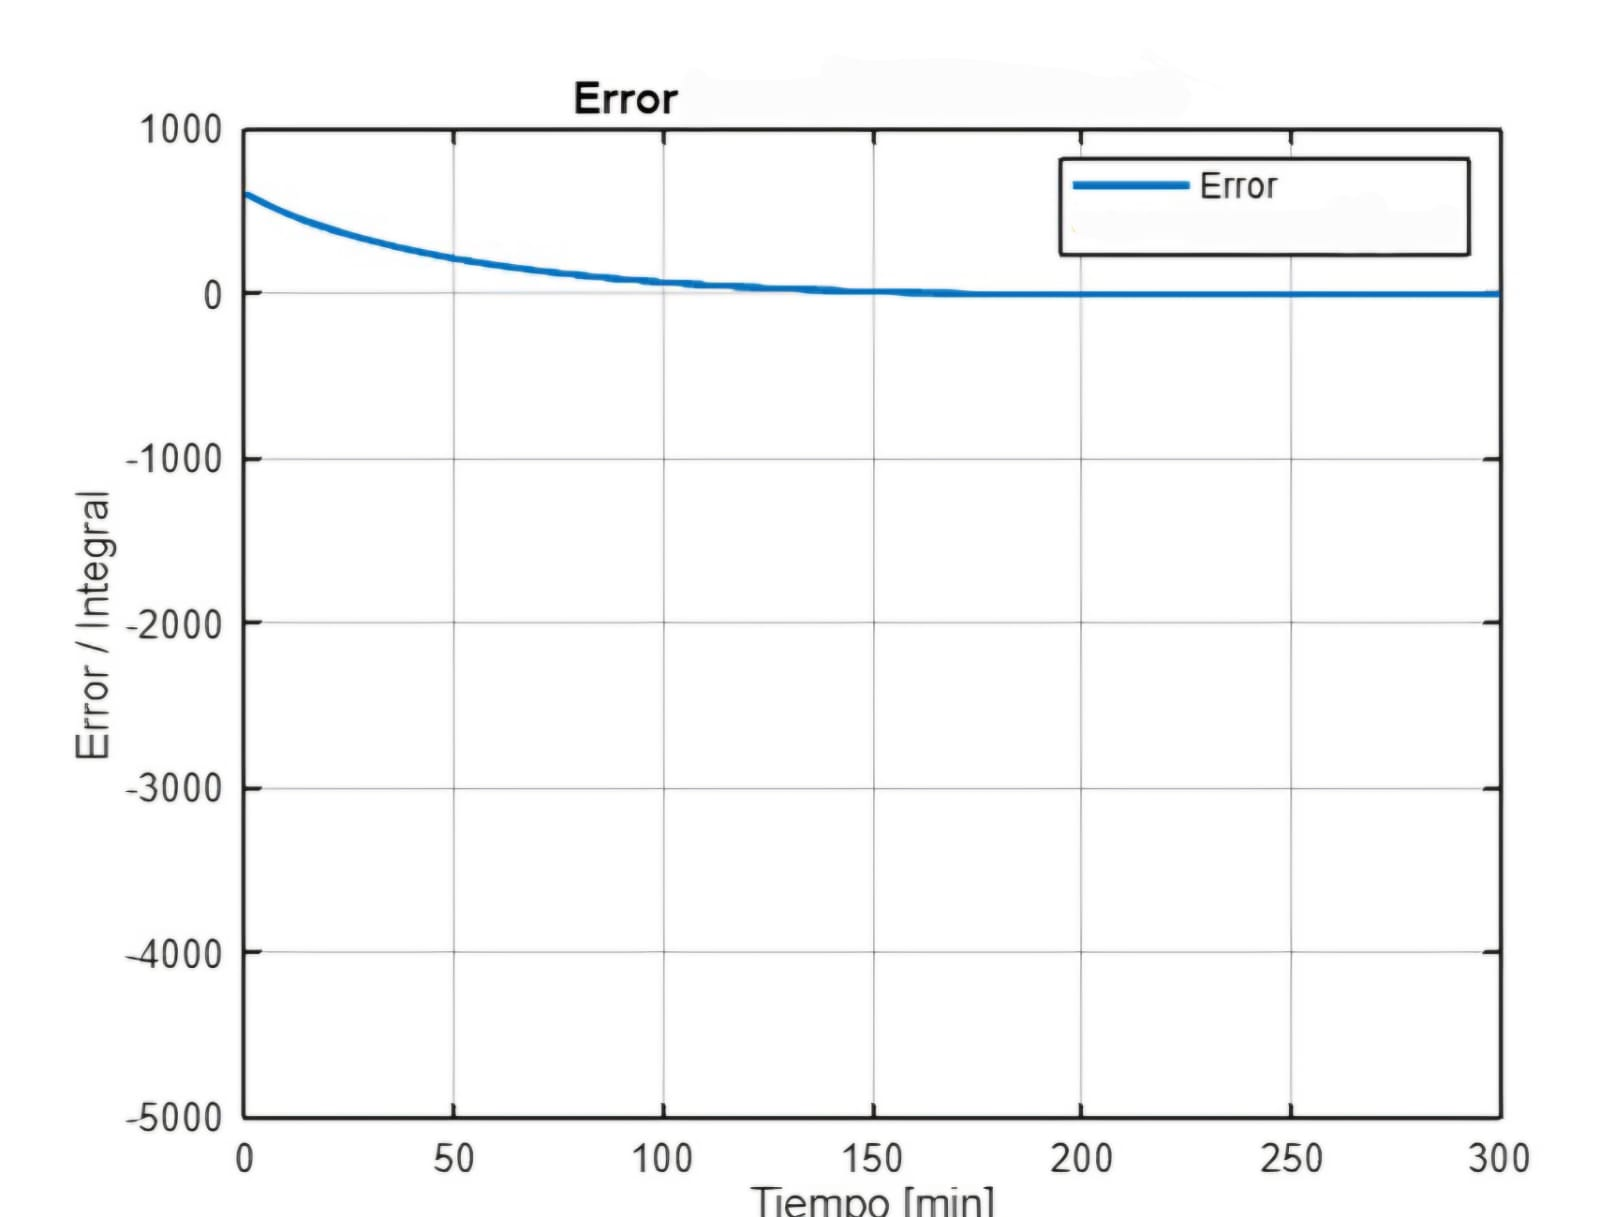
\includegraphics[width=0.9\linewidth]{images/capitulo4/FUZZY_Error_Simulacion.jpg}
    \caption{Evolución del error de control durante la simulación del controlador Fuzzy PI base.}
    \label{fig:fuzzy_error_simulacion}
\end{figure}

La Figura \ref{fig:fuzzy_error_simulacion} muestra la evolución del error de control durante la simulación. Al inicio, el error es elevado, con un valor aproximado de 600 ppm, debido a que la concentración de CO\(_2\) se encuentra muy por encima del setpoint. A medida que avanza la ventilación, el error disminuye de forma gradual hasta aproximarse a cero alrededor de los 150 a 180 minutos. Luego, el error se vuelve ligeramente negativo durante un intervalo corto, lo cual coincide con la reducción de la concentración de CO\(_2\) por debajo del setpoint. Finalmente, el error tiende nuevamente a cero, evidenciando una estabilización progresiva del sistema.

\begin{figure}[H]
    \centering
    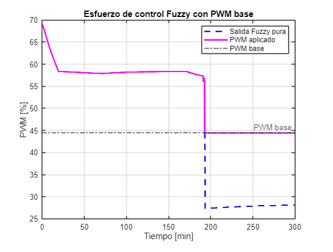
\includegraphics[width=0.9\linewidth]{images/capitulo4/FUZZY_Esfuerzo_Simulacion.png}
    \caption{Esfuerzo de control simulado del controlador Fuzzy PI base.}
    \label{fig:fuzzy_esfuerzo_simulacion}
\end{figure}

En la Figura \ref{fig:fuzzy_esfuerzo_simulacion} se observa el esfuerzo de control generado por el controlador Fuzzy PI. La salida Fuzzy pura inicia cerca del 69\% de PWM y disminuye rápidamente hasta una zona aproximada de 58\% durante los primeros minutos. Posteriormente, la acción de control se mantiene casi constante entre 57\% y 59\% hasta cerca de los 180 minutos, lo cual indica una actuación moderada y sostenida de los ventiladores. Cuando el sistema se aproxima al setpoint, la salida Fuzzy pura disminuye bruscamente hasta valores cercanos al 27\% o 28\%. Sin embargo, debido a la incorporación de un PWM base, el PWM aplicado se mantiene alrededor de 44\% a 45\%, evitando que la ventilación caiga por debajo del caudal mínimo requerido para sostener la concentración de CO\(_2\) cercana al valor de referencia.

\begin{figure}[H]
    \centering
    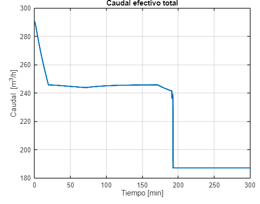
\includegraphics[width=0.9\linewidth]{images/capitulo4/FUZZY_Caudal_Simulacion.png}
    \caption{Caudal efectivo simulado generado por el sistema de ventilación con controlador Fuzzy PI base.}
    \label{fig:fuzzy_caudal_simulacion}
\end{figure}

La Figura \ref{fig:fuzzy_caudal_simulacion} presenta el caudal efectivo total generado por el sistema de ventilación. Al inicio de la simulación, el caudal se encuentra cerca de 290 m\(^3\)/h y disminuye rápidamente hasta aproximadamente 245 m\(^3\)/h durante los primeros minutos. Luego, el caudal se mantiene prácticamente estable entre 242 y 245 m\(^3\)/h hasta cerca de los 180 minutos. Al aproximarse la concentración de CO\(_2\) al setpoint, el caudal disminuye de forma abrupta hasta un valor cercano a 187 m\(^3\)/h, manteniéndose estable durante la etapa final de la simulación. Este comportamiento es coherente con la reducción del esfuerzo de control observada en la Figura \ref{fig:fuzzy_esfuerzo_simulacion}.

En conjunto, los resultados de simulación del controlador Fuzzy PI base muestran una respuesta estable, suave y progresiva para la reducción de CO\(_2\). El sistema logra aproximarse al setpoint de 900 ppm en un tiempo estimado de 170 a 180 minutos, con un esfuerzo de control moderado y sostenido durante la mayor parte de la simulación. En comparación con el controlador PI/PID simulado, el Fuzzy PI base presenta una respuesta más lenta, pero utiliza un menor esfuerzo inicial de ventilación, ya que no requiere mantener el PWM en 100\% durante la etapa inicial. Esto lo convierte en una estrategia menos agresiva, pero más gradual en términos de actuación sobre los ventiladores.


\subsection{Resultados de simulación del controlador Fuzzy PI agresivo}

En esta sección se presentan los resultados obtenidos mediante la simulación del controlador Fuzzy PI agresivo. Esta variante fue diseñada con el propósito de incrementar la acción de ventilación ante errores medios y altos de concentración de CO\(_2\), utilizando una base de reglas más intensa y una salida difusa orientada a mayores valores de PWM. De esta manera, se busca reducir el tiempo de llegada a la zona cercana al setpoint, aunque con un mayor esfuerzo de control respecto al Fuzzy PI base.

\begin{figure}[H]
    \centering
    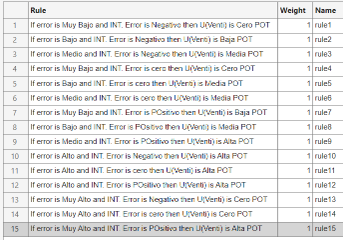
\includegraphics[width=0.9\linewidth]{images/capitulo4/Fuzzy_Agresivo_Reglas_Simulacion.png}
    \caption{Base de reglas utilizada en la simulación del controlador Fuzzy PI agresivo.}
    \label{fig:fuzzy_agresivo_reglas_simulacion}
\end{figure}

La Figura \ref{fig:fuzzy_agresivo_reglas_simulacion} muestra la base de reglas utilizada para la variante agresiva del controlador Fuzzy PI. En esta configuración, las combinaciones asociadas a errores medios, altos y muy altos generan con mayor frecuencia salidas de potencia media o alta. Esto permite que el sistema incremente la ventilación en etapas tempranas de la simulación, especialmente cuando la concentración de CO\(_2\) se encuentra considerablemente por encima del valor de referencia.

\begin{figure}[H]
    \centering
    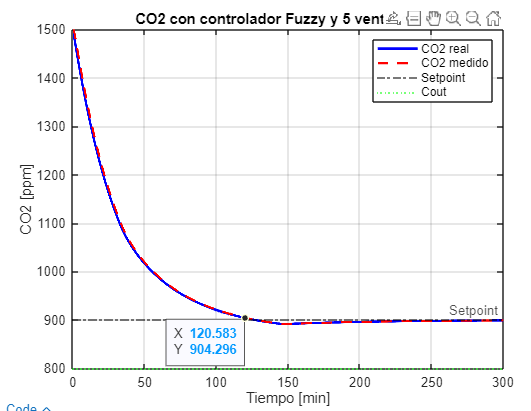
\includegraphics[width=0.9\linewidth]{images/capitulo4/Fuzzy_Agresivo_CO2_Simulacion.png}
    \caption{Respuesta simulada de la concentración de CO\(_2\) con controlador Fuzzy PI agresivo.}
    \label{fig:fuzzy_agresivo_co2_simulacion}
\end{figure}

Como se observa en la Figura \ref{fig:fuzzy_agresivo_co2_simulacion}, la concentración de CO\(_2\) inicia en un valor cercano a 1500 ppm y disminuye de forma sostenida debido a la acción del controlador. La respuesta ingresa a una zona cercana al setpoint alrededor de los 120.6 minutos, donde la concentración medida es aproximadamente 904.296 ppm. Posteriormente, el sistema continúa reduciendo ligeramente la concentración hasta ubicarse por debajo del valor de referencia, para luego estabilizarse gradualmente en torno a 900 ppm. En comparación con el Fuzzy PI base, esta variante alcanza la zona cercana al setpoint en menor tiempo, evidenciando una respuesta más rápida.

\begin{figure}[H]
    \centering
    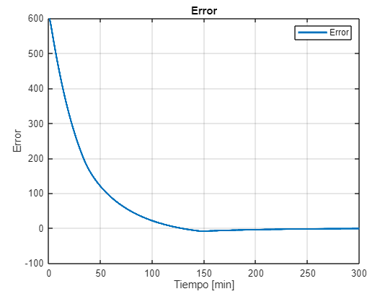
\includegraphics[width=0.9\linewidth]{images/capitulo4/Fuzzy_Agresivo_Error_Simulacion.png}
    \caption{Evolución del error de control durante la simulación del controlador Fuzzy PI agresivo.}
    \label{fig:fuzzy_agresivo_error_simulacion}
\end{figure}

La Figura \ref{fig:fuzzy_agresivo_error_simulacion} presenta la evolución del error de control. Al inicio de la simulación, el error es aproximadamente de 600 ppm, debido a que la concentración inicial de CO\(_2\) se encuentra muy por encima del setpoint. Durante los primeros minutos, el error disminuye rápidamente como consecuencia del mayor esfuerzo de ventilación aplicado por el controlador agresivo. Cerca de los 120 a 150 minutos, el error se aproxima a cero y posteriormente toma valores ligeramente negativos, lo que indica que la concentración de CO\(_2\) desciende temporalmente por debajo del valor de referencia. Finalmente, el error tiende nuevamente a cero, mostrando la estabilización progresiva del sistema.

\begin{figure}[H]
    \centering
    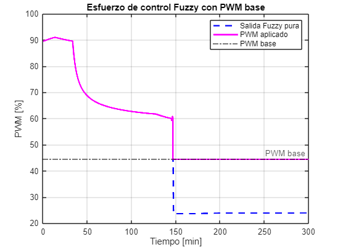
\includegraphics[width=0.9\linewidth]{images/capitulo4/Fuzzy_Agresivo_Esfuerzo_Simulacion.png}
    \caption{Esfuerzo de control simulado del controlador Fuzzy PI agresivo.}
    \label{fig:fuzzy_agresivo_esfuerzo_simulacion}
\end{figure}

En la Figura \ref{fig:fuzzy_agresivo_esfuerzo_simulacion} se muestra el esfuerzo de control generado por el controlador Fuzzy PI agresivo. Durante la etapa inicial, el PWM aplicado se mantiene cercano al 90\%, lo que refleja una acción de ventilación más intensa que la observada en el Fuzzy PI base. Luego, la señal disminuye progresivamente hasta valores cercanos al 60\% alrededor de los 140 minutos. Cuando el sistema alcanza la zona del setpoint, la salida Fuzzy pura cae hasta aproximadamente 24\% a 25\%; sin embargo, debido al PWM base, el PWM aplicado se mantiene alrededor de 44\% a 45\%. Este comportamiento permite conservar una ventilación mínima para sostener la concentración de CO\(_2\) cerca del valor objetivo.

\begin{figure}[H]
    \centering
    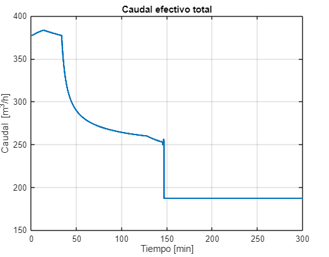
\includegraphics[width=0.9\linewidth]{images/capitulo4/Fuzzy_Agresivo_Caudal_Simulacion.png}
    \caption{Caudal efectivo simulado generado por el sistema de ventilación con controlador Fuzzy PI agresivo.}
    \label{fig:fuzzy_agresivo_caudal_simulacion}
\end{figure}

La Figura \ref{fig:fuzzy_agresivo_caudal_simulacion} muestra el caudal efectivo total producido por los ventiladores durante la simulación. Al inicio, el caudal se encuentra aproximadamente entre 375 y 380 m\(^3\)/h, valor superior al observado en el Fuzzy PI base. Posteriormente, el caudal disminuye de manera progresiva conforme la concentración de CO\(_2\) se aproxima al setpoint, ubicándose cerca de 260 m\(^3\)/h alrededor de los 120 a 140 minutos. Finalmente, cuando la respuesta entra en la zona cercana al valor de referencia, el caudal desciende abruptamente hasta aproximadamente 188 m\(^3\)/h, manteniéndose estable durante la etapa final de la simulación. Esta evolución es coherente con la disminución del esfuerzo de control mostrada previamente.

En conjunto, los resultados de simulación del controlador Fuzzy PI agresivo muestran una respuesta más rápida que la obtenida con el Fuzzy PI base. La concentración de CO\(_2\) ingresa a una zona cercana al setpoint aproximadamente a los 120.6 minutos, frente al comportamiento más lento del Fuzzy PI base. No obstante, esta mejora en rapidez se obtiene a costa de un mayor esfuerzo inicial de control, ya que el PWM aplicado inicia cerca del 90\% y el caudal efectivo alcanza valores próximos a 380 m\(^3\)/h. Por ello, esta variante puede considerarse más adecuada cuando se prioriza una reducción más rápida de CO\(_2\), aunque implica una mayor demanda de ventilación durante la etapa inicial.


\subsection{Resultados de simulación del controlador LQR}

En esta sección se presentan los resultados obtenidos mediante la simulación del controlador LQR aplicado al modelo de concentración de CO\(_2\) del aula. Esta estrategia de control se basa en la realimentación de estados y busca regular la ventilación considerando un compromiso entre la rapidez de respuesta y el esfuerzo de control aplicado. Para la simulación se mantuvieron las mismas condiciones generales empleadas en las estrategias anteriores, considerando una concentración inicial elevada de CO\(_2\), un setpoint de 900 ppm y la actuación de cinco ventiladores.

\begin{figure}[H]
    \centering
    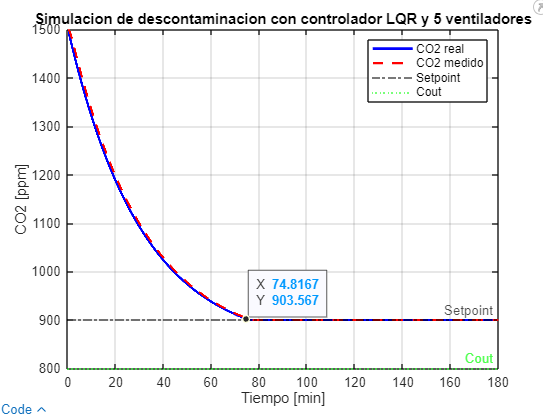
\includegraphics[width=0.9\linewidth]{images/capitulo4/LQR_CO2_Simulacion.png}
    \caption{Respuesta simulada de la concentración de CO\(_2\) con controlador LQR.}
    \label{fig:lqr_co2_simulacion}
\end{figure}

Como se observa en la Figura \ref{fig:lqr_co2_simulacion}, la concentración de CO\(_2\) inicia en un valor cercano a 1500 ppm y disminuye progresivamente debido a la acción del controlador LQR. La respuesta alcanza una zona cercana al setpoint alrededor de los 74.8 minutos, donde la concentración medida es aproximadamente 903.567 ppm. Posteriormente, el sistema continúa acercándose al valor de referencia de 900 ppm sin presentar oscilaciones importantes. Este comportamiento evidencia que el controlador LQR permite reducir la concentración de CO\(_2\) de manera estable y con un tiempo de respuesta menor al observado en los controladores Fuzzy PI base y Fuzzy PI agresivo.

\begin{figure}[H]
    \centering
    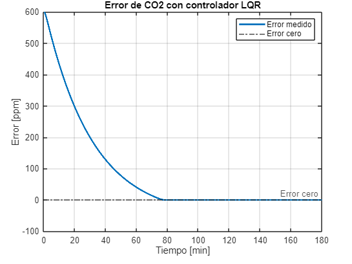
\includegraphics[width=0.9\linewidth]{images/capitulo4/LQR_Error_Simulacion.png}
    \caption{Evolución del error de control durante la simulación del controlador LQR.}
    \label{fig:lqr_error_simulacion}
\end{figure}

La Figura \ref{fig:lqr_error_simulacion} muestra la evolución del error de CO\(_2\) durante la simulación. Al inicio, el error es aproximadamente de 600 ppm, debido a la diferencia entre la concentración inicial de 1500 ppm y el setpoint de 900 ppm. Conforme actúa el sistema de ventilación, el error disminuye de forma continua hasta aproximarse a cero alrededor de los 75 minutos. A diferencia de otras respuestas, no se observa un sobrepaso negativo considerable, lo cual indica que el sistema se aproxima al valor de referencia de manera controlada y estable.

\begin{figure}[H]
    \centering
    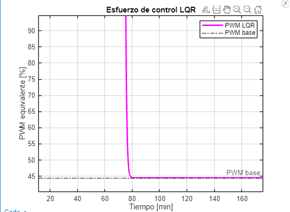
\includegraphics[width=0.9\linewidth]{images/capitulo4/LQR_Esfuerzo_Simulacion.png}
    \caption{Esfuerzo de control simulado del controlador LQR.}
    \label{fig:lqr_esfuerzo_simulacion}
\end{figure}

En la Figura \ref{fig:lqr_esfuerzo_simulacion} se presenta el esfuerzo de control generado por el controlador LQR, expresado como PWM equivalente. Durante la etapa inicial de la simulación, el PWM aplicado se mantiene en un valor elevado, cercano al 90\%, debido a que la concentración de CO\(_2\) se encuentra muy por encima del setpoint. Alrededor de los 75 minutos, cuando el sistema se aproxima al valor de referencia, el esfuerzo de control disminuye rápidamente hasta ubicarse cerca del PWM base, aproximadamente entre 44\% y 45\%. Esto indica que el controlador reduce la ventilación una vez alcanzada la zona objetivo, manteniendo solo la acción necesaria para sostener la concentración cercana al setpoint.

\begin{figure}[H]
    \centering
    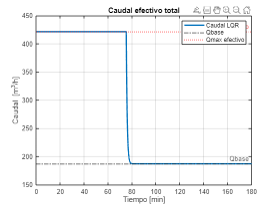
\includegraphics[width=0.9\linewidth]{images/capitulo4/LQR_Caudal_Simulacion.png}
    \caption{Caudal efectivo simulado generado por el sistema de ventilación con controlador LQR.}
    \label{fig:lqr_caudal_simulacion}
\end{figure}

La Figura \ref{fig:lqr_caudal_simulacion} muestra el caudal efectivo total generado por los ventiladores durante la simulación. En la etapa inicial, el caudal se mantiene aproximadamente en 420 m\(^3\)/h, correspondiente a una alta demanda de ventilación para reducir rápidamente la concentración de CO\(_2\). Cuando el sistema se aproxima al setpoint, cerca de los 75 minutos, el caudal disminuye de manera abrupta hasta un valor cercano a 188 m\(^3\)/h. Este valor se mantiene prácticamente constante durante la etapa final, lo cual es coherente con la reducción del esfuerzo de control observada en la Figura \ref{fig:lqr_esfuerzo_simulacion}.

En conjunto, los resultados de simulación del controlador LQR muestran una respuesta estable y rápida frente a una concentración inicial elevada de CO\(_2\). El sistema alcanza una zona cercana al setpoint aproximadamente a los 74.8 minutos, con una concentración de 903.567 ppm, y luego se estabiliza alrededor del valor de referencia sin oscilaciones significativas. En comparación con los controladores Fuzzy PI base y Fuzzy PI agresivo, el LQR presenta un menor tiempo de llegada a la zona objetivo. Sin embargo, esta mejora se obtiene mediante un esfuerzo inicial elevado, con un PWM cercano al 90\% y un caudal aproximado de 420 m\(^3\)/h durante la etapa inicial. Por ello, el controlador LQR representa una estrategia eficiente para reducir el tiempo de mitigación, manteniendo una respuesta estable después de alcanzar el setpoint.


\subsection{Comparación general de los controladores simulados}

Con el propósito de evaluar el desempeño de las estrategias de control implementadas en simulación, se realizó una comparación entre el controlador PI/PID, el controlador Fuzzy PI base, el controlador Fuzzy PI agresivo y el controlador LQR. Para esta comparación se consideraron criterios como el tiempo aproximado de llegada a la zona cercana al setpoint, el esfuerzo inicial de control, el caudal efectivo inicial, la estabilidad de la respuesta y la observación general del comportamiento de cada estrategia.

\begin{table}[H]
    \centering
    \renewcommand{\arraystretch}{1.4}
    \caption{Comparación de desempeño de los controladores simulados}
    \label{tabla:comparacion_controladores_simulados}
    \resizebox{\textwidth}{!}{
    \begin{tabular}{|p{3cm}|p{3cm}|p{3cm}|p{3cm}|p{4.5cm}|}
        \hline
        \textbf{Controlador} & \textbf{Tiempo aprox. de llegada al setpoint} & \textbf{Esfuerzo inicial de control} & \textbf{Caudal inicial aprox.} & \textbf{Observación general} \\ \hline

        PI/PID & 60.3 min & 100\% PWM & 515 m\(^3\)/h & Presenta la respuesta más rápida en simulación, pero requiere la actuación máxima de los ventiladores durante la etapa inicial. \\ \hline

        Fuzzy PI base & 170--180 min & 69\% PWM aprox. & 290 m\(^3\)/h & Presenta una respuesta más lenta, pero con una acción de control más suave y menor demanda inicial de ventilación. \\ \hline

        Fuzzy PI agresivo & 120.6 min & 90\% PWM aprox. & 375--380 m\(^3\)/h & Mejora el tiempo de respuesta respecto al Fuzzy PI base, pero incrementa el esfuerzo de control y la ventilación inicial. \\ \hline

        LQR & 74.8 min & 90\% PWM aprox. & 420 m\(^3\)/h & Presenta una respuesta rápida y estable, con menor tiempo que los controladores Fuzzy y sin oscilaciones significativas. \\ \hline

    \end{tabular}
    }
\end{table}

Como se observa en la Tabla \ref{tabla:comparacion_controladores_simulados}, el controlador PI/PID alcanza la zona cercana al setpoint en el menor tiempo, aproximadamente a los 60.3 minutos. Este resultado se debe a que el controlador mantiene una actuación máxima durante la etapa inicial, con un PWM cercano al 100\% y un caudal efectivo aproximado de 515 m\(^3\)/h. Por ello, aunque presenta la reducción más rápida de CO\(_2\), también es la estrategia con mayor exigencia inicial sobre los ventiladores.

El controlador Fuzzy PI base presenta el comportamiento más conservador. Su tiempo de llegada a la zona cercana al setpoint se encuentra aproximadamente entre 170 y 180 minutos, lo que evidencia una respuesta más lenta frente a la concentración inicial elevada de CO\(_2\). Sin embargo, este controlador utiliza un esfuerzo inicial menor, cercano al 69\% de PWM, y un caudal inicial aproximado de 290 m\(^3\)/h. Esto indica que su acción de ventilación es más gradual, por lo que puede ser útil en escenarios donde se prioriza una actuación menos agresiva del sistema.

Por otro lado, el controlador Fuzzy PI agresivo mejora el desempeño del Fuzzy PI base al reducir el tiempo de llegada a la zona cercana al setpoint hasta aproximadamente 120.6 minutos. Esta mejora se obtiene mediante una mayor acción de control inicial, con un PWM cercano al 90\% y un caudal efectivo aproximado entre 375 y 380 m\(^3\)/h. En ese sentido, esta variante representa un punto intermedio entre el Fuzzy PI base y las estrategias más rápidas, ya que reduce el tiempo de mitigación, pero aumenta el esfuerzo de ventilación.

Finalmente, el controlador LQR alcanza una zona cercana al setpoint alrededor de los 74.8 minutos, con una concentración aproximada de 903.567 ppm. Su respuesta es más rápida que la de los controladores Fuzzy PI base y Fuzzy PI agresivo, y se mantiene estable luego de aproximarse al valor de referencia. Aunque también requiere un esfuerzo inicial elevado, cercano al 90\% de PWM, su comportamiento muestra una transición ordenada hacia el PWM base, lo que evidencia un buen compromiso entre rapidez y estabilidad.

En conjunto, la comparación permite identificar que el controlador PI/PID ofrece la mayor rapidez de mitigación, mientras que el Fuzzy PI base presenta la actuación más suave. El Fuzzy PI agresivo mejora el tiempo de respuesta del controlador difuso, aunque con mayor esfuerzo inicial. Por su parte, el LQR muestra un desempeño equilibrado, ya que logra una respuesta rápida y estable sin presentar oscilaciones significativas. Por ello, la selección de la estrategia más adecuada dependerá del criterio priorizado: rapidez de reducción de CO\(_2\), suavidad de actuación, estabilidad o consumo energético asociado a la ventilación.




\section{Resultados experimentales del controlador PI/PID}

En esta sección se presentan los resultados experimentales obtenidos durante la implementación del controlador PI/PID para la mitigación activa de CO\(_2\). La prueba permitió analizar la evolución de la concentración de CO\(_2\), el error de control, el esfuerzo aplicado por el controlador, el caudal efectivo estimado y la respuesta en RPM del ventilador monitoreado.

\begin{figure}[H]
    \centering
    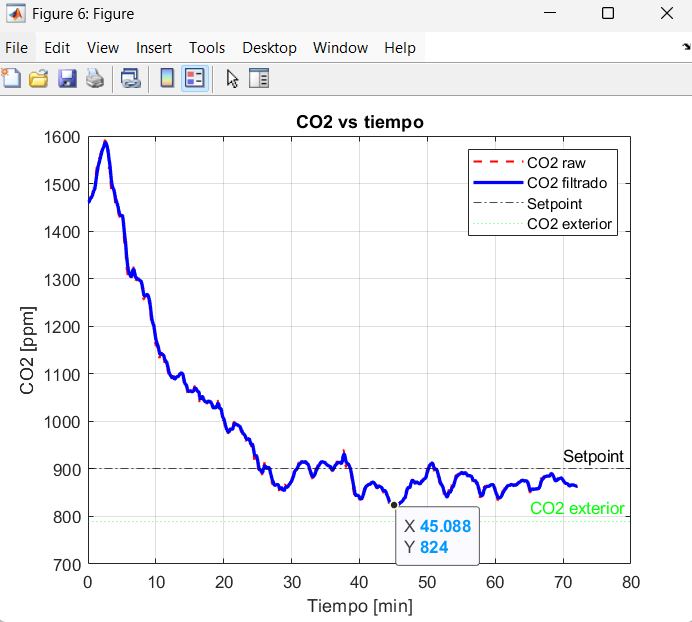
\includegraphics[width=0.9\linewidth]{images/capitulo4/CO2vsTiempo.png}
    \caption{Evolución de la concentración de CO\(_2\) durante la prueba experimental con controlador PI/PID.}
    \label{fig:pid_co2_tiempo}
\end{figure}

Como se observa en la Figura \ref{fig:pid_co2_tiempo}, la concentración de CO\(_2\) inicia en un valor elevado, cercano a 1500 ppm, y posteriormente disminuye de manera progresiva debido a la acción de los ventiladores. El sistema logra aproximarse al setpoint establecido de 900 ppm y luego se mantiene en una zona cercana o inferior a dicho valor. Este comportamiento evidencia que el controlador PI/PID permite reducir la concentración de CO\(_2\) desde una condición inicial desfavorable hasta un rango más adecuado para el ambiente evaluado.

\begin{figure}[H]
    \centering
    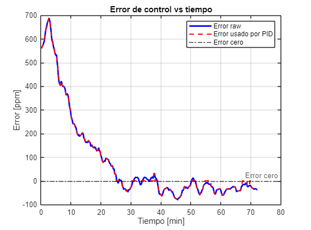
\includegraphics[width=0.9\linewidth]{images/capitulo4/ERRORvsTiempo.png}
    \caption{Evolución del error de control durante la prueba experimental con controlador PI/PID.}
    \label{fig:pid_error_tiempo}
\end{figure}

La Figura \ref{fig:pid_error_tiempo} muestra la evolución del error de control, calculado como la diferencia entre la concentración medida de CO\(_2\) y el setpoint. Al inicio de la prueba, el error es elevado debido a que la concentración de CO\(_2\) se encuentra por encima del valor de referencia. Conforme avanza la ventilación, el error disminuye progresivamente hasta aproximarse a cero. Las oscilaciones posteriores alrededor del error nulo pueden atribuirse al ruido del sensor, a la dinámica propia del ambiente y a las variaciones generadas por la actuación de los ventiladores.

\begin{figure}[H]
    \centering
    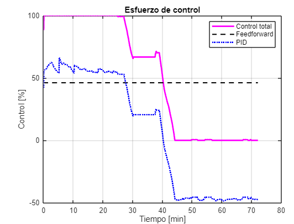
\includegraphics[width=0.9\linewidth]{images/capitulo4/EsfuerzoControl.png}
    \caption{Esfuerzo de control aplicado por el controlador PI/PID.}
    \label{fig:pid_esfuerzo_control}
\end{figure}

En la Figura \ref{fig:pid_esfuerzo_control} se presenta el esfuerzo de control aplicado al sistema. Durante la etapa inicial, la señal de control total se mantiene en valores elevados, debido a que la concentración de CO\(_2\) supera ampliamente el setpoint. A medida que la concentración disminuye, el esfuerzo de control también se reduce, lo cual indica que el controlador disminuye progresivamente la ventilación cuando el sistema se aproxima al valor de referencia.

\begin{figure}[H]
    \centering
    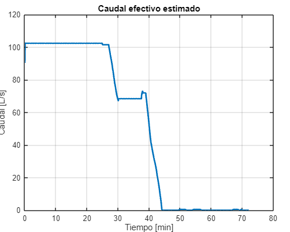
\includegraphics[width=0.9\linewidth]{images/capitulo4/Caudal.png}
    \caption{Caudal efectivo estimado durante la prueba experimental con controlador PI/PID.}
    \label{fig:pid_caudal}
\end{figure}

La Figura \ref{fig:pid_caudal} muestra el caudal efectivo estimado a partir de la señal de control aplicada a los ventiladores. Al inicio de la prueba, el caudal se mantiene en un valor alto debido a la necesidad de reducir rápidamente la concentración de CO\(_2\). Posteriormente, conforme el sistema se acerca al setpoint, el caudal disminuye hasta valores cercanos a cero. Este resultado es coherente con la reducción del esfuerzo de control observada previamente.

\begin{figure}[H]
    \centering
    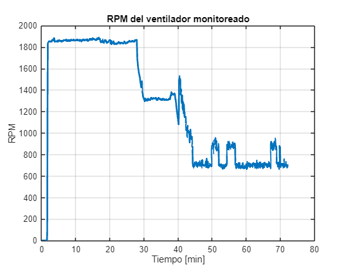
\includegraphics[width=0.9\linewidth]{images/capitulo4/RPM.png}
    \caption{RPM del ventilador monitoreado durante la prueba experimental con controlador PI/PID.}
    \label{fig:pid_rpm}
\end{figure}

Finalmente, la Figura \ref{fig:pid_rpm} presenta la velocidad de giro del ventilador monitoreado. Se observa que, durante los primeros minutos, las RPM se mantienen en valores elevados, lo cual coincide con la alta señal de control aplicada por el controlador. Luego, conforme disminuye el requerimiento de ventilación, las RPM también se reducen. Esta gráfica permite validar que la señal PWM generada por el sistema tiene un efecto directo sobre la actuación física del ventilador.

En conjunto, los resultados experimentales muestran que el controlador PI/PID implementado permite reducir la concentración de CO\(_2\) hasta una zona cercana al setpoint y ajustar progresivamente la ventilación aplicada. Además, las gráficas de esfuerzo de control, caudal y RPM permiten verificar que la disminución de CO\(_2\) está asociada a una actuación real de los ventiladores. No obstante, se observan pequeñas oscilaciones alrededor del valor de referencia, las cuales pueden relacionarse con el ruido de medición, la dinámica del ambiente y la sensibilidad del sistema frente a cambios en la señal PWM.




\section{Página web para la lectura de los sensores}



\customchapter{CONCLUSIONES Y RECOMENDACIONES} 

\section{Conclusiones}

\begin{itemize}
    \item \textbf{Diseño de la arquitectura de red IoT y software:} Se diseñó una arquitectura para la red IoT como para la aplicación de monitoreo, empleando una topología estrella para las conexiones entre los nodos sensores y el gateway. La integración de nodos sensores con comunicación LoRa y una plataforma de visualización basada en tecnologías web modernas garantiza la escalabilidad y facilidad de mantenimiento del sistema.
    
    \item \textbf{Implementación de la red de nodos sensores:} Los nodos sensores se implementaron con éxito utilizando módulos LoRa para la transmisión de datos y sensores de CO\(_2\) de alta precisión. Este diseño permite capturar y transmitir datos de forma eficiente y remota, validando la funcionalidad de los sensores y la transmisión en condiciones controladas.
    
    \item \textbf{Desarrollo de la plataforma de software:} Se desarrolló una aplicación web funcional para la visualización y almacenamiento de los datos en tiempo real, con un sistema de alertas que notifica al usuario cuando los niveles de CO\(_2\) superan los límites definidos. La implementación de gráficos históricos y un dashboard centralizado facilita el monitoreo y la toma de decisiones informadas.
    
    \item \textbf{Configuración del gateway Kona Mega:} Aunque no se logró completar la configuración del gateway Kona Mega, se avanzó en la documentación y comprensión de sus requisitos y protocolos de comunicación. Esto permitirá que la integración final sea más eficiente en futuros trabajos.
    
    \item \textbf{Pruebas individuales exitosas:} Las pruebas individuales de los nodos sensores y de la plataforma de software demostraron que cada componente del sistema cumple con sus requisitos de diseño. Sin embargo, la falta de pruebas del sistema completamente integrado limita la validación del flujo de datos entre los nodos sensores, el gateway y la aplicación web.
    
    \item \textbf{Limitaciones y próximos pasos:} La ausencia de pruebas de integración debido a la falta de configuración del gateway no permitió culminar el trabajo verificando la funcionalidad total del sistema; sin embargo, se logró documentar parte de esta configuración.
\end{itemize}

\section{Recomendaciones}

\begin{itemize}
    \item \textbf{Priorizar la configuración del gateway Kona Mega:} Completar la configuración del gateway Kona Mega es esencial para realizar pruebas de integración y validar el flujo de datos desde los nodos sensores hasta la plataforma web. Se recomienda seguir las guías del fabricante y estableces comunicación con el soporte técnico debido a que el material disponible en la web es escaso y/o de difícil acceso.
    
    \item \textbf{Pruebas de integración del sistema completo:} Una vez configurado el gateway, es crucial realizar pruebas exhaustivas de todo el sistema, desde la captura de datos en los nodos sensores hasta su visualización en la plataforma web. Esto permitirá identificar y resolver problemas potenciales de conectividad o procesamiento; así como reconocer áreas de mejora del proyecto.
    
    \item \textbf{Documentar las configuraciones y resultados:} Es importante mantener una documentación clara de las configuraciones realizadas en el gateway y los nodos sensores, así como de los resultados de las pruebas de integración. Esto facilitará futuras implementaciones y replicación del proyecto.
    
    \item \textbf{Optimización del sistema de alertas:} Evaluar y mejorar el sistema de alertas, incluyendo ajustes en los umbrales de CO\(_2\) mediante un perfil de administrador dentro de la aplicación, y pruebas de diferentes formas de notificación (ventanas emergentes, correos electrónicos, notificaciones móviles), para garantizar que las alertas sean efectivas y rápidas.
    
    \item \textbf{Ampliación del sistema:} Una vez que el sistema esté completamente integrado y probado, se recomienda explorar la posibilidad de agregar más nodos sensores y extender el alcance de la red IoT para monitorear múltiples aulas o espacios de manera simultánea. Si bien el coste del tipo de sensor utilizado es alto, el proyecto claramente documentado es altamente replicable para otro tipo de aplicaciones que involucren recolección de data de sensores y comunicación inalámbrica. Por otra parte, sería recomendable hacer un presupuesto y mostrar la arquitectura que se utilizaría en caso de escalar el proyecto para múltiples áreas de la universidad.
\end{itemize}

\phantomsection
\addcontentsline{toc}{section}{\bfseries REFERENCIAS BIBLIOGRÁFICAS}
\markboth{REFERENCIAS BIBLIOGRÁFICAS}{REFERENCIAS BIBLIOGRÁFICAS}

\renewcommand{\bibname}{\vspace*{-2\baselineskip}\hfill\Large\bf{REFERENCIAS BIBLIOGRÁFICAS}\hfill}
%\renewcommand{\bibname}{\hfill\Large\bf{REFERENCIAS BIBLIOGRÁFICAS}\hfill}

\bibliographystyle{IEEEtran} % Estableciendo el estilo de citas IEEEtram.

\bibliography{referencias} % Recibe las referencias de IEEE

\appendix
\chapter{Código para el nodo sensor}
\label{anexo:codigo_nodo}
A continuación se proporciona el enlace al repositorio que contiene el código fuente en C/C++ (Arduino) desarrollado para la placa Arduino UNO del nodo sensor. Este código incluye las rutinas de lectura de los sensores de CO\(_2\), temperatura, humedad, el control del actuador PWM y el empaquetado de la telemetría.

\begin{center}
    URL del repositorio: \href{https://github.com/sebasandre2020/Tesis-2026-1/tree/appCode/Codes/Nodes/main}{https://github.com/sebasandre2020/Tesis-2026-1/tree/appCode/Codes/Nodes/main}
\end{center}

\chapter{Código para el gateway personalizado}
\label{anexo:codigo_gateway}
Este anexo contiene el enlace al código fuente en C/C++ desarrollado para el microcontrolador ESP32 que actúa como gateway. Incluye las clases \texttt{LoRaManager} y \texttt{AzureIoTManager} encargadas de la recepción LoRa en modo no bloqueante y la publicación MQTT segura hacia Azure IoT Hub.

\begin{center}
    URL del repositorio: \href{https://github.com/sebasandre2020/Tesis-2026-1/tree/appCode/Codes/Gateway/main}{https://github.com/sebasandre2020/Tesis-2026-1/tree/appCode/Codes/Gateway/main}
\end{center}

\chapter{Código para la aplicación web}
\label{anexo:codigo_web}
A continuación se provee el enlace al código fuente de la plataforma web, subdividido en el \textit{backend} (desarrollado en .NET Core 8.0 utilizando Clean Architecture) y el \textit{frontend} (desarrollado en React).

\begin{center}
    URL del repositorio: \href{https://github.com/sebasandre2020/Tesis-2026-1/tree/appCode/Codes/Frontend}{https://github.com/sebasandre2020/Tesis-2026-1/tree/appCode/Codes/Frontend}
\end{center}

\chapter{Código IaC para infraestructura en Azure}
\label{anexo:codigo_iac}
Este anexo contiene el enlace a los \textit{scripts} y plantillas de Infraestructura como Código (IaC), utilizados para el aprovisionamiento y configuración automatizada de los recursos en Microsoft Azure (IoT Hub, SQL Database, Container Apps, Azure Functions, Static Web Apps, etc.).

\begin{center}
    URL del repositorio: \href{https://github.com/sebasandre2020/Tesis-2026-1/tree/appCode/Codes/Software\%20Infraestructure}{https://github.com/sebasandre2020/Tesis-2026-1/tree/appCode/Codes/Software\%20Infraestructure}
\end{center}

\chapter{Acceso a la aplicación web desplegada}
\label{anexo:acceso_web}
Este anexo proporciona el enlace de acceso directo a la aplicación web de monitoreo y alerta ambiental desplegada en producción en Microsoft Azure.

\begin{center}
    URL de la aplicación: \href{https://orange-pond-0bd85900f.7.azurestaticapps.net/}{https://orange-pond-0bd85900f.7.azurestaticapps.net/}
\end{center}

\end{document}
